\PassOptionsToPackage{svgnames,dvipsnames}{xcolor}

%% add the masters option to print master of science
\documentclass[12pt,masters]{cmuthesis}

\usepackage[Lenny]{fncychap}
\ChNameVar{\Large}

\usepackage[%
    colorlinks=true,allcolors=link_color,pageanchor=true,%
    plainpages=false,pdfpagelabels,bookmarks,bookmarksnumbered,%
]{hyperref}

\usepackage[style=alphabetic,natbib=true,backend=biber,maxnames=10]{biblatex}
\bibliography{refs.bib}

\usepackage{totcount}
\newtotcounter{citenum}
\AtEveryBibitem{\stepcounter{citenum}}

\DeclareFieldFormat{citehyperref}{%
    \DeclareFieldAlias{bibhyperref}{noformat}% Avoid nested links
    \bibhyperref{#1}}

\DeclareFieldFormat{textcitehyperref}{%
    \DeclareFieldAlias{bibhyperref}{noformat}% Avoid nested links
    \bibhyperref{%
        #1%
        \ifbool{cbx:parens}
        {\bibcloseparen\global\boolfalse{cbx:parens}}
        {}}}

\savebibmacro{cite}
\savebibmacro{textcite}

\renewbibmacro*{cite}{%
    \printtext[citehyperref]{%
        \restorebibmacro{cite}%
        \usebibmacro{cite}}}

\renewbibmacro*{textcite}{%
    \ifboolexpr{
        ( not test {\iffieldundef{prenote}} and
        test {\ifnumequal{\value{citecount}}{1}} )
        or
        ( not test {\iffieldundef{postnote}} and
        test {\ifnumequal{\value{citecount}}{\value{citetotal}}} )
    }
    {\DeclareFieldAlias{textcitehyperref}{noformat}}
    {}%
    \printtext[textcitehyperref]{%
        \restorebibmacro{textcite}%
        \usebibmacro{textcite}}}


\usepackage{fullpage}
\usepackage{graphicx}
\usepackage{amsmath}
\definecolor{link_color}{RGB}{0,128,255}

\usepackage[%
    letterpaper,twoside,vscale=.8,hscale=.75,nomarginpar,hmarginratio=1:1
]{geometry}

\usepackage{graphicx} % more modern
% \usepackage{subfigure}
\usepackage{subcaption}

\setlength {\marginparwidth }{2cm}
\usepackage{todonotes}
\newcommand{\todon}[1]{\todo[color=red!40,inline,size=\small]{TODO: #1}}
\newcommand{\todoc}{\todo[color=red!40,inline,size=\small]{TODO: Complete}}

\usepackage{amsmath}
\usepackage{amssymb}
\usepackage{amsthm}
\usepackage{arydshln}
\usepackage{thm-restate}


\usepackage{accents}
\newcommand{\ubar}[1]{\underaccent{\bar}{#1}}

\usepackage{stackengine}

% \usepackage{wrapfig}
\usepackage{enumitem,wrapfig,adjustbox,multirow}


\newtheorem{proposition}{Proposition}
\newtheorem{assumption}{Assumption}
\newtheorem{theorem}{Theorem}
\newtheorem{corollary}{Corollary}
\newtheorem{lemma}[theorem]{Lemma}

% \MakeRobust{\Call}
\newcommand*\Let[2]{\State #1 $\gets$ #2}

\definecolor{lightgray}{gray}{0.95} % 10%

\usepackage{algorithm}
\usepackage{algorithmicx}

\usepackage{hyperref}
\renewcommand{\theHalgorithm}{\arabic{algorithm}}


\usepackage{easytable}

\usepackage[capitalise,nameinlink,noabbrev]{cleveref}

\usepackage{stmaryrd}


\usepackage{algpseudocode}
\algnewcommand{\LeftComment}[1]{\Statex \(\triangleright\) #1}

\newcounter{module}
\makeatletter
\newenvironment{module}[1][htb]{%
    \let\c@algorithm\c@module
    \renewcommand{\ALG@name}{Module}%
    \begin{algorithm}[#1]%
        }{\end{algorithm}}
\makeatother
\crefname{module}{Module}{Modules}

\usepackage{booktabs}

\usepackage{caption}

\usepackage{listings,textcomp,color}
\definecolor{backcolour}{rgb}{0.95,0.95,0.92}
\definecolor{deepblue}{rgb}{0,0,0.5}
\definecolor{deepred}{rgb}{0.6,0,0}
\lstset{language=Python,upquote=true,
    basicstyle=\ttfamily\footnotesize,
    commentstyle=\textit,stringstyle=\upshape,
    numbers=left,numberstyle=\footnotesize,stepnumber=1,numbersep=5pt,
    backgroundcolor=\color{backcolour},frame=single,tabsize=2,
    showspaces=false,showstringspaces=false,showtabs=false,
    breaklines=true,breakatwhitespace=true,escapeinside=||,
    emph={cp, torch, cpth},emphstyle=\color{deepred},
    keywordstyle=\color{deepblue},
}

% Python style for highlighting
% \DeclareFixedFont{\ttm}{T1}{txtt}{m}{n}{12}  % for normal
% \definecolor{deepgreen}{rgb}{0,0.5,0}
% \lstset{
% language=Python,
% basicstyle=\ttm,
% otherkeywords={self},             % Add keywords here
% keywordstyle=\ttb\color{deepblue},
% emph={cp},          % Custom highlighting
% emphstyle=\ttb\color{deepred},    % Custom highlighting style
% stringstyle=\color{deepgreen},
% frame=tb,                         % Any extra options here
% showstringspaces=false            %
% }

\usepackage{xspace}

\usepackage{framed}


%%% Local Variables:
%%% coding: utf-8
%%% mode: latex
%%% TeX-engine: xetex
%%% TeX-master: "../thesis"
%%% End:
\DeclareMathOperator*{\argmax}{argmax}
\DeclareMathOperator*{\argmin}{argmin}
\DeclareMathOperator*{\diag}{diag} \DeclareMathOperator*{\tr}{tr}
\DeclareMathOperator*{\maximize}{maximize}
\DeclareMathOperator*{\minimize}{minimize}
\DeclareMathOperator*{\st}{s.t.}
\DeclareMathOperator*{\subjectto}{subject\;to}
\DeclareMathOperator*{\vect}{vec} \DeclareMathOperator*{\mat}{mat}
\DeclareMathOperator{\prox}{prox}
\DeclareMathAlphabet\mathbfcal{OMS}{cmsy}{b}{n}

\newcommand{\I}{\mathcal{I}}
\newcommand{\J}{\mathcal{J}}
\newcommand{\RR}{\mathbb{R}}
\newcommand{\R}{\mathbb{R}}
\newcommand{\dd}{\mathsf{d}}
\newcommand{\DD}{\mathsf{D}}

% \newcommand{\nwc}{\newcommand}
% \DeclareMathOperator*{\maximize}{maximize}
% \DeclareMathOperator{\prox}{prox}
% \DeclareMathOperator*{\argmin}{argmin}
% \DeclareMathOperator*{\argmax}{argmax}
% \DeclareMathOperator*{\minimize}{minimize}
% \DeclareMathOperator*{\subjectto}{subject\;to}
% \DeclareMathOperator*{\st}{s.t.}

% \newcommand{\uu}{\bm{u}}
% \newcommand{\U}{\mathcal{U}}
% \newcommand{\fix}{\marginpar{FIX}}
% \newcommand{\new}{\marginpar{NEW}}
% \newcommand{\x}{\bm{x}}
% \newcommand{\X}{\mathcal{X}}
\newcommand{\D}{\mathcal{D}}
\newcommand{\X}{\mathcal{X}}
\newcommand{\Y}{\mathcal{Y}}
% \newcommand{\s}{\bm{s}}
% \newcommand{\aaa}{\bm{a}}
% \newcommand{\mmu}{\bm{\mu}}
\newcommand{\E}{\mathbb{E}}
% \newcommand{\f}{\bm{f}}
% \newcommand{\F}{\bm{F}}
% \newcommand{\kk}{\bm{k}}
% \newcommand{\PP}{\bm{P}}
% \newcommand{\vv}{\bm{v}}
% \newcommand{\MM}{\bm{M}}
\newcommand{\LL}{\mathcal{L}}
\newcommand{\JJ}{\mathcal{J}}
\newcommand{\ZZ}{\mathbb{Z}}

\newcommand{\xinit}{x_{\rm init}}
\newcommand{\uinit}{u_{\rm init}}
\newcommand{\ustar}{{u^\star}}
\newcommand{\vstar}{{v^\star}}
\newcommand{\sstar}{{s^\star}}
\newcommand{\xstar}{{x^\star}}
\newcommand{\ystar}{{y^\star}}
\newcommand{\zstar}{{z^\star}}

\newcommand{\CC}{\mathcal{C}}
\newcommand{\K}{\mathcal{K}}
% \newcommand{\RR}{\mathbb{R}}
% \newcommand{\ZZ}{\mathbb{Z}}
\newcommand{\Res}{\mathcal{R}}

\newcommand{\menge}[2]{\big\{{#1}~\big |~{#2}\big\}}

\newcommand{\eg}{{\it e.g.}\xspace}
\newcommand{\ie}{{\it i.e.}\xspace}

\newcommand{\LQR}{\ensuremath{\mathrm{LQR}}}
\newcommand{\MPC}{\ensuremath{\mathrm{MPC}}}

\newcommand{\LML}{\ensuremath{\mathcal{L}}}
\newcommand{\cvxpy}{\texttt{cvxpy}\xspace}
\newcommand{\qpth}{\texttt{qpth}\xspace}
% \newcommand{\intexp}{\texttt{Internet Explorer}\xspace}
\newcommand{\intexp}{\textbf{Internet Explorer}\xspace}

\newcommand{\cblock}[3]{
  \hspace{-1.5mm}
  \begin{tikzpicture}
    [
    node/.style={square, minimum size=10mm, thick, line width=0pt},
    ]
    \node[fill={rgb,255:red,#1;green,#2;blue,#3}] () [] {};
  \end{tikzpicture}%
}


\draftstamp{\today}{DRAFT}

\begin{document}
\frontmatter

\pagestyle{empty}

\title{{\bf Online Representation Learning on the Open Web}}
\author{Ellis L. Brown, II}
\date{May 2023}
\Year{2023}
\trnumber{CMU-CS-23-1XX}

\committee{
    \begin{tabular}{rl}
        Deepak Pathak           & \textit{Carnegie Mellon University} \hspace{0.5em}  (chair)\\
        Deva Ramanan            & \textit{Carnegie Mellon University} \\
        Alexei A.\ Efros         & \textit{University of California, Berkeley} \\
    \end{tabular}
}

\support{}
\disclaimer{}

\keywords{
    machine learning,
    deep learning,
    computer vision,
    representation learning,
    self-supervised learning,
    active learning,
    online learning,
    internet
}

\maketitle


\begin{dedication}
    To my parents, John and Amy, for their unwavering support and love, \\
    and to Mara for putting up with all of the madness.

\end{dedication}


\begin{abstract}
    Domain-specific modeling priors and specialized components are
    becoming increasingly important to the machine learning field.
    These components integrate specialized knowledge that we have
    as humans into model.
    We argue in this thesis that optimization methods provide an
    expressive set of operations that should be part of the
    machine learning practitioner's modeling toolbox.

    We present two foundational approaches for optimization-based modeling:
    1) the \emph{OptNet} architecture that integrates
    optimization problems as individual layers in larger end-to-end
    trainable deep networks, and
    2) the \emph{input-convex neural network (ICNN)}
    architecture that helps make inference and learning in deep
    energy-based models and structured prediction more tractable.

    We then show how to use the OptNet approach
    1) as a way of combining model-free and model-based reinforcement
    learning and
    2) for top-$k$ learning problems.
    We conclude by showing how to differentiate cone programs
    and turn the \cvxpy domain specific language into
    a differentiable optimization layer that enables rapid prototyping of
    the approaches in this thesis. \\

    \noindent
    The source code for this thesis document is available in open source form at:
    \begin{center}
        \url{https://github.com/ellisbrown/cmu-masters-thesis}
    \end{center}
\end{abstract}

% \newgeometry{left=0.5in,right=0.5in,top=1in,bottom=1.4in}
\begin{acknowledgments}
    I have been incredibly fortunate and privileged throughout my life to have been given many opportunities that have led me to pursue this thesis research. Thanks to all of the people who have provided me with the environment, safety, health, financial well-being, love, joy, support, and knowledge to produce this work.

    First and foremost, I would like to thank my advisor, Deepak Pathak, for his guidance, support, and mentorship throughout my Masters.
    I am incredibly thankful for the unparalleled opportunities he has given me to grow as a researcher, and for taking an early bet on me.
    I would also like to thank my close collaborator, Alyosha Efros, for his mentorship and guidance throughout my Masters. It has been an incredible experience to learn from and work with him.
    I would also like to thank Deva Ramanan for taking the time to serve on my committee and providing early feedback on my work.

    % Alex Li (phd student of deepak's), co-author of our internet explorer project --- served as a mentor, collaborator, and great friend throughout my masters.
    Next, I would like to give a special thanks to Alex Li for his mentorship, guidance, collaboration, and friendship throughout my Masters. I could not have asked for a better collaborator on the Internet work---I hope that we have the opportunity to work together again in the future.

    Thanks to all of my other close friends at CMU in Smith Hall, NSH, and beyond for making my time here fly by. This includes (in alphabetic order)
    Ananye Agarwal,
    Sacha Bartholme,
    Shikhar Bahl,
    Sudeep Dasari,
    Shivam Duggal,
    Xuxin Cheng,
    Zipeng Fu,
    Helen Jiang,
    Aditya Kannan,
    Tanmay Kulkarni,
    Peter Manohar,
    Russell Mendonca,
    David Noursi,
    Nilay Pande,
    Mihir Prabhudesai,
    Alvin Shek,
    Aaron Trowbridge,
    Shagun Uppal,
    Haoyu Xiong,
    Jason Zhang,
    and many others.

    Looking back, my teachers and mentors earlier in my life ignited my interests in computer science and mathematics and later opened my eyes to the world of research.
    In high school,
    I was fortunate to have wonderful mathematics teachers in
    Joan Llufrio and Amy Scheer, who taught me to love problem solving;
    at the same time, my water polo coach, Don Casey, taught me the importance of hard work, discipline, and delayed gratification.
    During undergrad at Vanderbilt,
    Gerald Roth and Graham Hemingway taught me to love computer science, and I will be forever grateful to Maithilee Kunda for taking a chance on me and introducing me to artificial intelligence and the world of research as a second semester senior.
    
    After Vanderbilt at BlackRock, I was fortunate to have the opportunity to work with an incredible cast of people at their AI Labs, who helped cement my desire to pursue graduate school. I am especially thankful to Rachel Schutt for selecting me as a founding member of the group, and for her mentorship and guidance throughout my time there. I am also thankful to my manager, Alex McKay, for his mentorship and guidance, and my close friends and colleagues, including
    Melanie Manko,
    Don Weidner,
    Mike Sereiko,
    Sri Bhupatiraju,
    Jeevan Acharya,
    Jason Motylinski,
    Shawn Simpson,
    Jack Gindi,
    Hristo Paskov,
    Nick Moehle,
    Steven Diamond,
    Shane Barrett,
    and others.
    I would also like to thank our senior advisors for their close guidance and support, including
    Mykel Kochenderfer,
    Stephen Boyd,
    Trevor Hastie,
    and Rob Tibshirani.

    I would be remiss not to mention the support I have received from the Native American community throughout my graduate school journey. From my first research presentation opportunity at AISES, the guidance on application procedures and personal mentorship, and financial support in the form of scholarships through AISES and the Osage Nation---it is safe to say that I would not be where I am today without this wonderful community.

    On the personal side, I would like to thank all of my other friends and family members that have provided me with an immense amount of love, support, and encouragement throughout the years---especially my girlfriend Mara, who has been by my side through it all.
    Thanks to my parents John and Amy;
    siblings Marnie and Evan;
    and the rest of my extended family
    for raising me in a wonderful environment and
    encouraging me at every step along the way.
\end{acknowledgments}
% \restoregeometry

\pagestyle{plain}

\tableofcontents
\addtocontents{toc}{\vspace*{-2cm}}
\listoffigures
\addtocontents{lof}{\vspace*{-2cm}}
\listoftables
\listofalgorithms

\mainmatter

\chapter{Introduction}

Suppose you have a small dataset and need to train a model for some task, say classification.
% How would you go about doing it?
A pipeline that has become standard today is to download the latest pre-trained deep network and fine-tune it on your own small dataset. This pre-trained model used to be ImageNet-based~\cite{deng2009imagenet,he2016deep} and now would probably be CLIP~\cite{radford2021learning}. The implicit goal set by the community for such pre-trained models is that they should transfer well to any kind of downstream task not known in advance. This has led to a race to build ultra-large-scale models in terms of computation, model size, and dataset size. But is this goal of building an ``omniscient'' pre-trained model that can work on any future downstream task even feasible? Perhaps not because our world is continually changing.
Although the size of the pretraining datasets has grown from 1.2M~~\cite{deng2009imagenet} to 400M~\cite{schuhmann2021laion} images, what has not changed at all is their nature: these datasets are curated, and, more importantly, \textit{\textbf{static}}. For instance, the portion of ImageNet curated before 2007 has no idea what an iPhone is.
% "static": Jason, to me, this is the most important part of the motivation. size of the dataset is not that important since we already have such big datasets that we only train 1-2 epochs on. the main issue with these datasets is that they are fixed in time. ontologies change rapidly (eg new products come out), category meanings might change (eg what a smartphone looks like is different in 2023 vs 2013), new words may even develop (eg slay). I think the focus should be on training a static dataset by design will produce an outdated model. this isn't really mentioned until paragraph 2 and stays kinda vague
Furthermore, although a few hundred million images represent a staggering quantity of visual data, they are minuscule compared to the entire Internet, where billions of new photos are uploaded every day.
% , continuously updating with an incredible diversity of real-world objects and scenes.
Thus, current static datasets, however big they become,
% , are minuscule compared to the entire Internet, where billions of new photos are uploaded every day. They
fail to capture the richness and dynamic nature of the data available on the Internet.
% Not to mention the issue that the bigger we make our static pre-training datasets, the more compute burden they entail.
% that the compute scales with the size of the dataset as well.
Moreover, as our static datasets grow, they require increasingly inaccessible amounts of compute.

% So the ``big data'' in machine learning is easily dwarfed by the data generated collectively by the world. Furthermore, the bigger we make our static pre-training datasets, the more compute burden they entail: e.g., CLIP is trained on 256 GPUs for 12 days. 
% This begs the question: \textit{are static datasets, as big as they are, ever going to truly scale to capture the richness and dynamic nature of the data available on the Internet? }
% This begs the question: \textit{will static datasets, however big they become, ever truly scale to capture the richness and dynamic nature of the data available on the Internet? }
% We suspect that the answer is no, so what could be the alternative? % want to remove this sentence

\begin{figure}[t]
    \centering
    % \includegraphics{figures/fig1-cvpr-2022v3.pdf}
    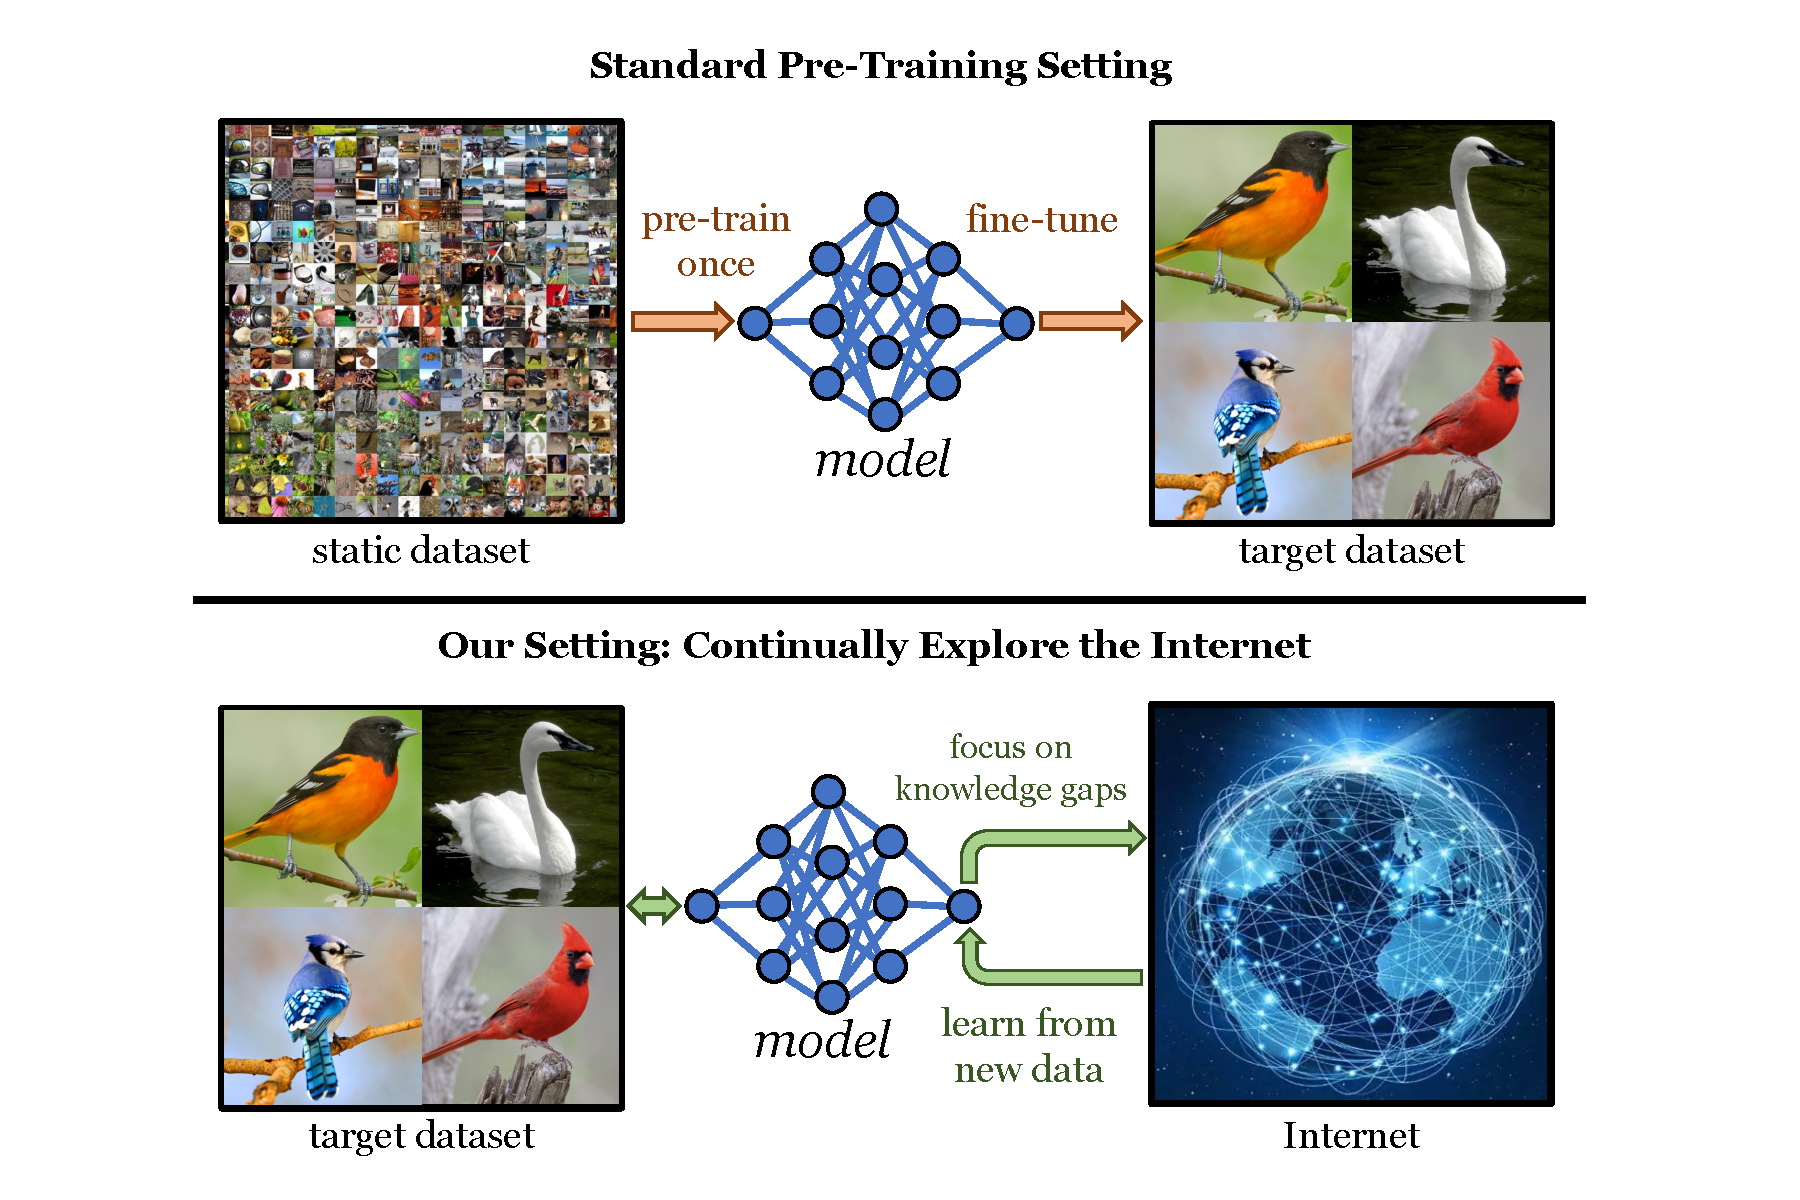
\includegraphics[width=0.8\linewidth]{figures/teaser2.pdf}
    % 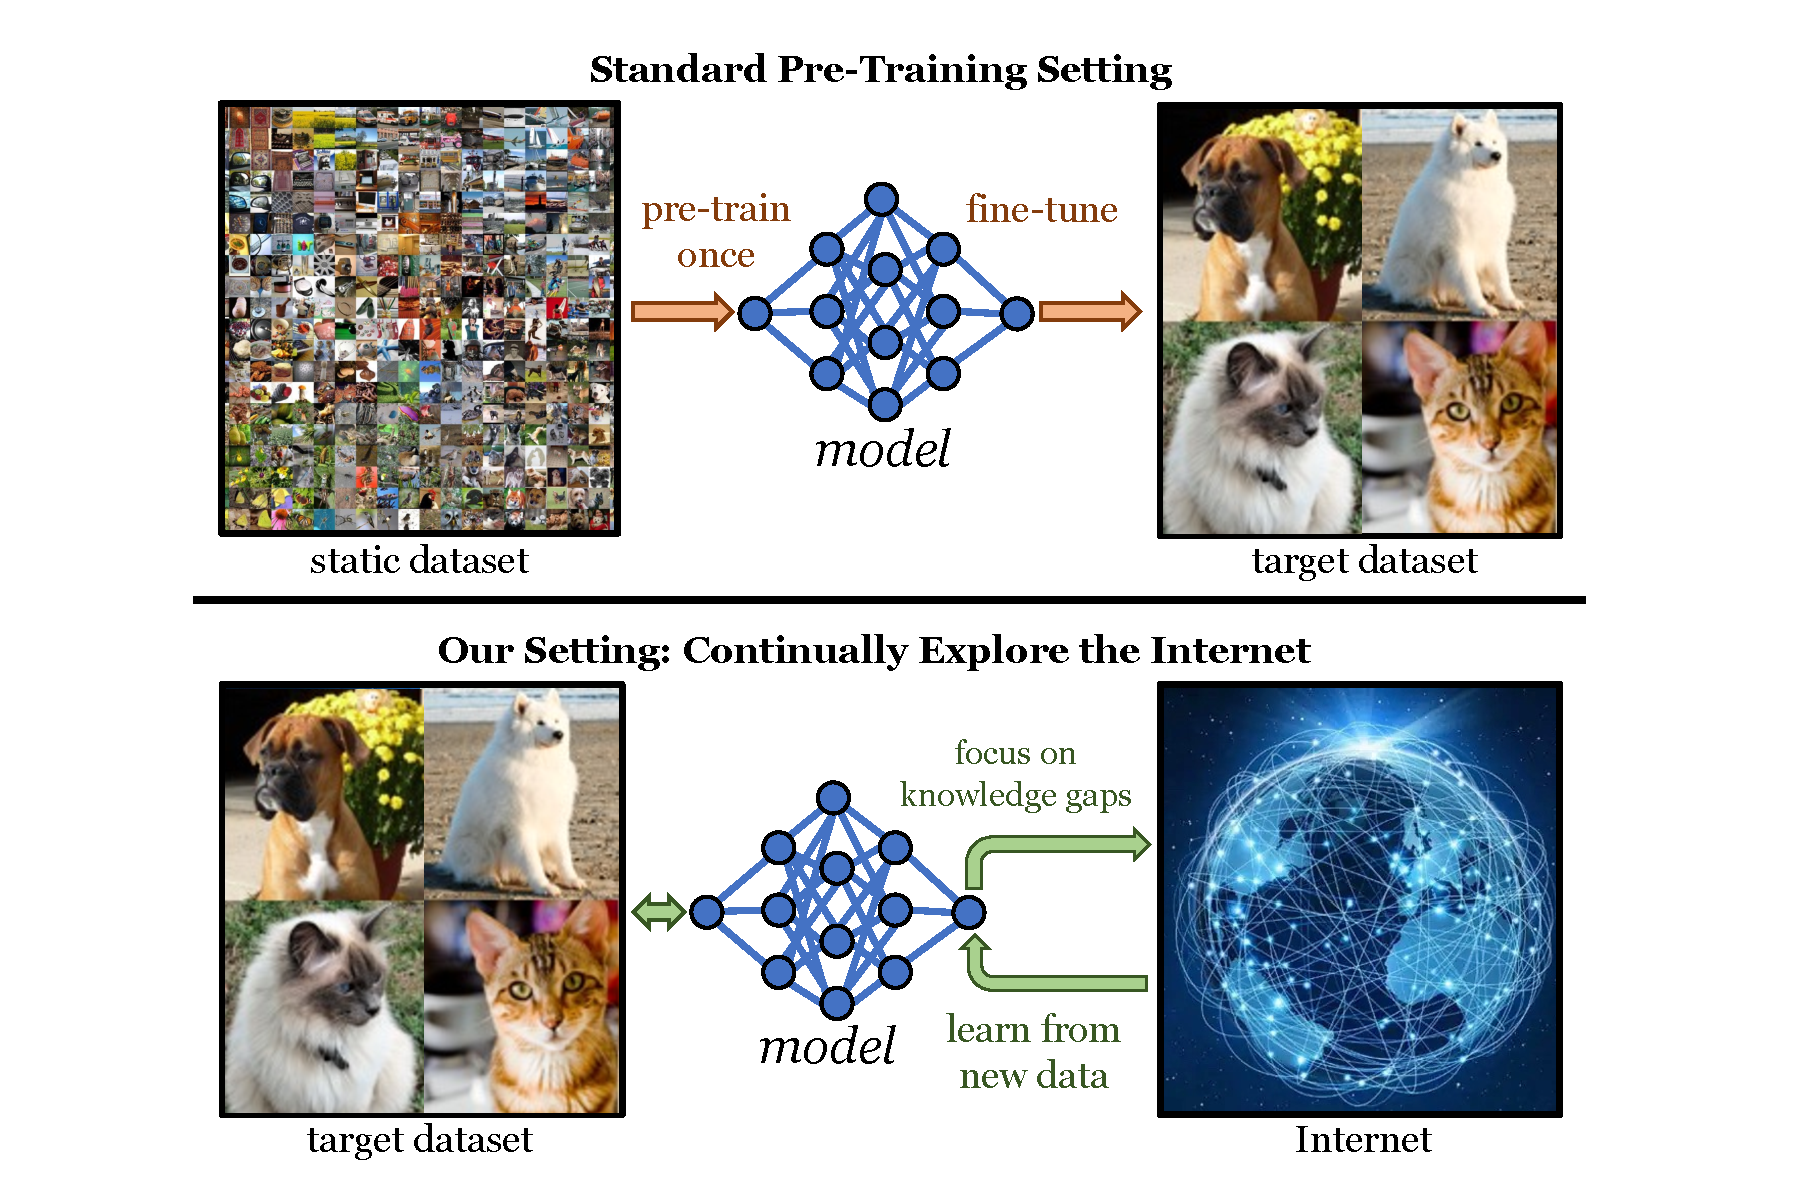
\includegraphics[width=\linewidth]{figures/alex.pdf}
    \caption{Given unlabeled data for a target task, our approach, Internet Explorer, searches the Internet to progressively find more and more relevant training data via self-supervised exploration.}
    \label{fig:teaser}
    % \vspace{-0.1in}
    \vspace{-0.15in}
\end{figure}

In this thesis, we rethink the idea of a \textit{\textbf{generic}} large-scale pretrained model and propose an alternate paradigm of training a rather small-scale but up-to-date model geared towards the \textit{\textbf{specific}} downstream task of interest. To train such a model, we go beyond static datasets and \textit{treat the Internet itself as a dynamic, open-ended dataset}. Unlike conventional datasets, which are expensive to increase and grow stale with time,
%are prone to bias, and yield suboptimal transfer performance when they contain little relevant data to the downstream task. 
the Internet is dynamic, rich, grows automatically, and is always up to date.
Its continuously evolving nature also means we cannot hope to ever download it or train a model, whether large or small, on all of it.
% But thinking pragmatically, do we even need to do so? Perhaps not.

We propose that the Internet can be treated as a special kind of dataset---one that exists out there, ready to be queried as needed to quickly train a customized model for a desired task.
% However, the issue is that the Internet is too big, and finding relevant images that help improve performance on a target dataset is a challenging endeavor.
We draw an analogy to reinforcement learning, where even though the task is known, finding a policy that can generate the desired behavior is non-trivial due to the high complexity of the state space. Hence, most approaches rely on some form of exploration to figure out what actions the agent should take so that it quickly finds high-reward states. Inspired by this analogy, we formulate a disembodied, online agent we call {\em Internet Explorer}, that actively searches the Internet using standard search engines to find relevant visual data that improve feature quality on a target dataset (see \cref{fig:teaser}). The agent's actions are text queries made to search engines, and the observations are the data obtained from the search.

The queries made by Internet Explorer improve over time. It cycles between searching for images on the Internet with text queries, self-supervised training on downloaded images, determining which images are relevant to the target dataset, and prioritizing what to search for next (see \cref{fig:method}). We also bootstrap Internet Explorer using existing pre-trained models such as MoCov3~\cite{he2020momentum} and obtain a significant boost on the target datasets.

Our setting is different from active learning~\cite{settles2009active}, where the goal is to selectively obtain labels for data points from a fixed dataset. In contrast, Internet Explorer continually expands the size of its dataset and requires no labels for training, even from the target dataset.
% However, we also show results in settings when the label set of the target dataset (not individual labels) are known.
Some prior works have also discussed ways to leverage the Internet as an additional source of data. NELL~\cite{carlson2010toward} proposed a way to continually scrape web pages to learn new concepts and relationships, which are periodically curated by a human in the loop. NEIL~\cite{chen2013neil} builds on the dictionary developed by NELL to search visual data to develop visual relationships. Both are semi-supervised methods to gather general ``common-sense'' knowledge from the Internet. In contrast, we perform an actively improving \textit{directed} search to perform well on target data, in a fully self-supervised manner. Recent work~\cite{jiang2021improving} follows a similar setting but searches a static dataset and not the Internet.

We evaluate Internet Explorer across 5 datasets, including 4 fine-grained datasets and PASCAL VOC.
% For simplicity, the search engine used is Google, but the method itself can work by searching on just image tags/captions as well.
We search for relevant images using Google; however, the method is compatible with any text-based search engine or even a static dataset (see \cref{subsec:search_engine_main}).
% \todo{prev sentence is out of date. mention laion / flickr}
We compare against several strong baselines, including CLIP, on downstream tasks. Note that CLIP acts as an oracle for our approach because it has likely already seen all or more queries that Internet Explorer makes.
In most scenarios, Internet Explorer either outperforms or matches CLIP oracle using only a single 3090 GPU desktop machine that runs for 30--40 hours, makes over 10K progressively improving queries, and downloads over 1M relevant Internet images for each target dataset.


\begin{figure}[t]
    \centering
    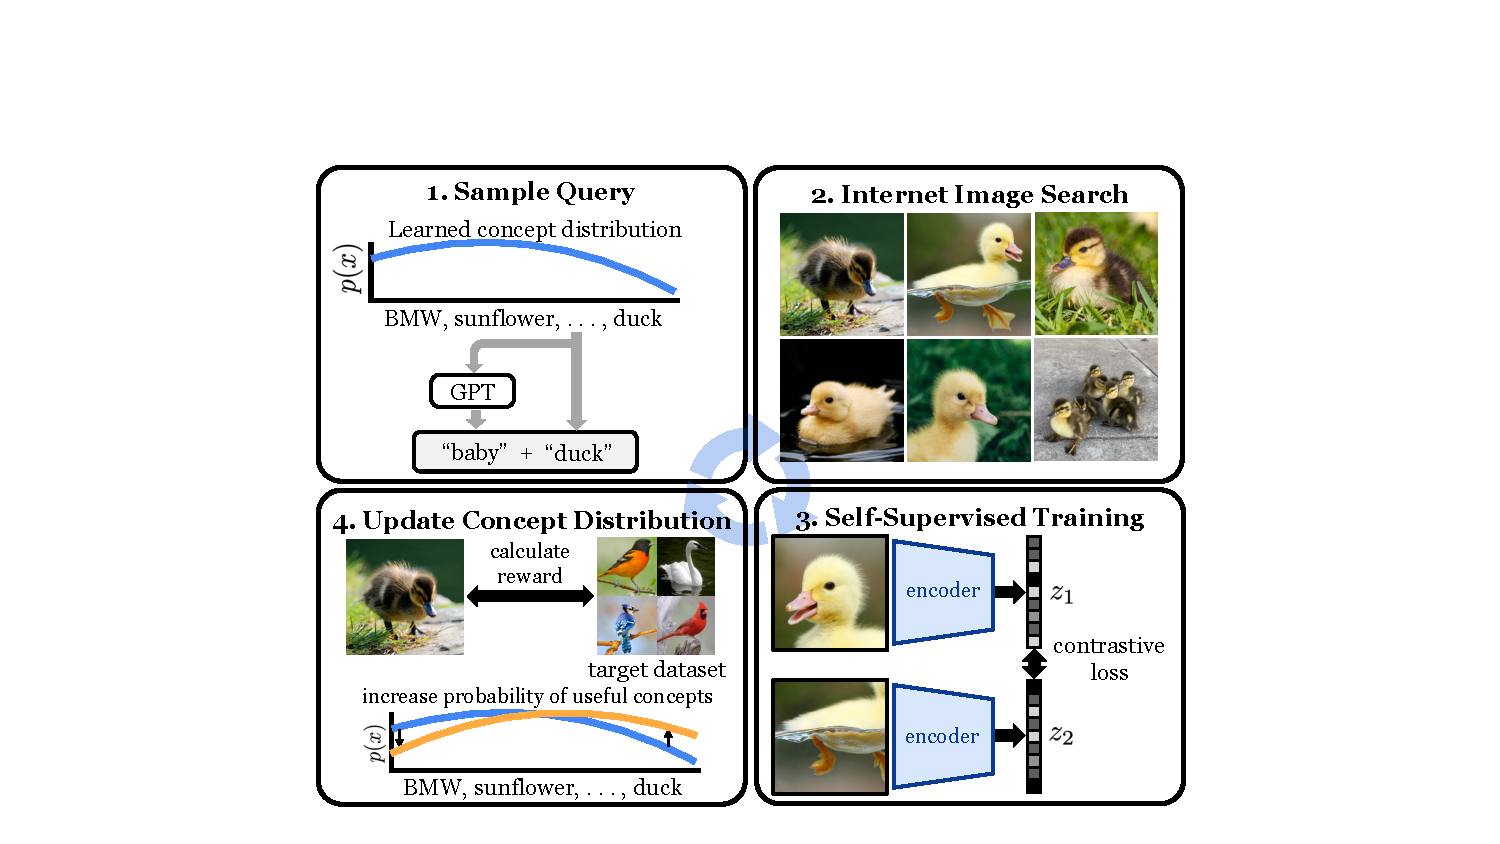
\includegraphics[width=0.85\linewidth]{figures/method_fig2.pdf}
    \caption{\textbf{Overview of Internet Explorer.} Our goal is to efficiently search the Internet for images that improve our performance on a target dataset.
        % In each iteration, we generate text queries by combining a concept sampled from a learned distribution with a GPT-generated descriptor. We query Google Images with the resulting phrase and download the top 100 image results. We add these images to the set of previously downloaded images and perform self-supervised learning on the combined dataset. 
        % Finally, we evaluate the relevance of the new images and increase the likelihood of the query and other related queries if the new images are similar to the target dataset.
        In each iteration, we first generate text queries by combining a concept sampled from a learned distribution with a GPT-generated descriptor (\S\ref{subsec:text_query_generation}, \ref{subsec:tiering}). Next, we query search engines with the resulting phrase and download the top 100 image results (\S\ref{subsec:text_to_image_search}, \ref{subsec:search_engine_main}). We add these images to the set of previously downloaded images and perform self-supervised training on the combined dataset (\S\ref{subsec:ssl}). Finally, we evaluate the relevance of the new images and update our concept distribution to increase the likelihood of similar queries if their images were similar to the target dataset (\S\ref{subsec:image_rel_reward},~\ref{subsec:unseen_reward}).
    }
    \label{fig:method}
    \vspace{-1em}
\end{figure}


%%% Local Variables:
%%% coding: utf-8
%%% mode: latex
%%% TeX-engine: xetex
%%% TeX-master: "../thesis"
%%% End:
\chapter{Preliminaries and Background}
This section provides a broad overview of foundational ideas
and background material relevant to this thesis.
In most chapters of this thesis, we include a deeper
discussion of the related literature relevant to
that material.

\section{Preliminaries}
The content in this thesis builds on the following topics.
We assume preliminary knowledge of these topics and
give a limited set of key references here.
The reader should have an understanding of statistical
and machine learning modeling paradigms as described in
\citet{wasserman2013all,bishop2007pattern,friedman2001elements}.
Our contributions mostly focus on end-to-end modeling with
deep architectures as described in
\citet{schmidhuber2015deep,goodfellow2016deep} with
applications in computer vision as described in
\citet{forsyth2003modern,bishop2007pattern,szeliski2010computer}.
Our contributions also involve optimization theory and
applications as described in
\citet{bertsekas1999nonlinear,boyd2004convex,bonnans2013perturbation,griewank2008evaluating,nocedal2006sequential,sra2012optimization,wright1997primal}.
One application area of this thesis work focuses on control
and reinforcement learning.
Control is one kind of optimization-based modeling and
is further described in
\citet{bertsekas2005dynamic,sastry2011adaptive,levine2017optimal}.
Reinforcement learning methods are summarized in
\citet{sutton1998reinforcement,levine2017introduction}.

\section{Energy-based Learning}
Energy-based learning is a machine learning method
typically used in supervised settings that explicitly
adds relationships and dependencies to the model's
output space.
This is in contrast to purely feed-forward models that
typically cannot explicitly capture dependencies
in the output space.
At the core of energy-based learning methods is
a scalar-valued \emph{energy} function
$E_\theta(x,y): \mathcal{X}\times\mathcal{Y}\rightarrow \mathbb{R}$
parameterized by $\theta$ that measures the fit
between some input $x$ and output $y$.
Inference in energy-based models is done by
solving the optimization problem
\begin{equation}
  \label{eq:bg:inf}
  \hat y = \argmin_{y} E_\theta(x, y).
\end{equation}
We note that this is a powerful formulation for
modeling and learning and subsumes the representational
capacity of standard deep feedforward models,
which we show how to do in \cref{sec:bg:ff-energy}.
The energy function can also be interpreted
from a probabilistic lens as the negated unnormalized
joint distribution over the input and output spaces.

Energy-based methods have been in use for over a decade
and the tutorial \citet{lecun2006tutorial} overviews
many of the foundational methods and challenges
in energy-based learning.
The two main challenges for energy-based learning are
1) learning the parameters $\theta$ of the energy
function $E_\theta$ and 2) efficiently solving
the inference procedure in \cref{eq:bg:inf}.
These challenges have historically been tamed by
using simpler energy functions consisting of
hand-engineered feature extractors for the inputs
$x$ and linear functions of $y$.
This captures models such as Markov random fields
\citep{li1994markov}
and conditional random fields
\citep{lafferty2001conditional,sutton2012introduction}.
Standard gradient-based methods are difficult to use
for parameter learning because $\hat y$ depends on $\theta$
through the $\argmin$ operator, which is not always differentiable.
Historically, a common approach to doing parameter learning
in energy-based models has been to directly shape the
energy function with a max-margin approach
\citet{taskar2004max,taskar2005learning}.

More recently, there has been a strong push to further incorporate
structured prediction methods like conditional random fields as the
``last layer'' of a deep network architecture
\citep{peng2009conditional,zheng2015conditional,chen2015learning}
as well as in deeper energy-based architectures
\citep{belanger2016structured,belanger2017end,belanger2017deep,wang2016proximal}.
We further discuss Structured Prediction Energy Networks (SPENs)
in \cref{sec:bg:spens}.

An ongoing discussion in the community argues whether
adding the dependencies explicitly in an energy-based is useful or not.
Feedforward models have a remarkable representational
capacity that can implicitly learn the dependencies and
relationships from data without needing to impose
additional structure or modeling assumptions and
without making the model more computationally
expensive with an optimization-based inference procedure.
One argument against this viewpoint that supports
energy-based modeling is that explicitly including
modeling information improves the data efficiency
and requires less samples to learn because some
structure and knowledge is already present in the model
and does not have to be learned from scratch.

\subsection{Energy-based Models Subsume Feedforward Models}
\label{sec:bg:ff-energy}
We highlight the power of energy-based modeling for supervised
learning by noting how they subsume deep feedforward models.
Let $\hat y = f_\theta(x)$ be a deep feedforward model.
The energy-based representation of this model is
$E(x,y) = ||y-f_\theta(x)||_2^2$
and inference becomes the convex optimization problem
$\hat y = \argmin_y E(x,y)$, which
has the exact solution $\hat y = f_\theta(x)$.
An energy function that has more structure over the output
space adds representational capacity that a feedforward
model wouldn't be able to capture explicitly.

\subsection{Structured Prediction Energy Networks}
\label{sec:bg:spens}
Structured Prediction Energy Networks (SPENs)
\citep{belanger2016structured,belanger2017end,belanger2017deep}
are a way of bridging the gap between modern deep
learning methods and classical energy-based learning
methods.
SPENs provide a deep structure over input and output spaces
by representing the energy function $E_\theta(x,y)$ with
a standard feed-forward neural network.
This expressive formulation comes at the cost of making
the inference procedure in \cref{eq:bg:inf} difficult
and non-convex.
SPENs typically use an approximate inference procedure
by taking a fixed-number of gradient descent steps
for inference.
For learning, SPENs typically replace the inference with
an \emph{unrolled gradient-based optimizer}
that starts with some prediction $y_0$ and
takes a fixed number of gradient steps to minimize
the energy function
$$y_{i+1} = y_i - \alpha \nabla_y E_\theta(x,y_i).$$
The final iterate as then taken as the prediction
$\hat y \triangleq y_N$.
Gradient-based parameter learning can be done by
differentiating the prediction $\hat y$ with respect
to $\theta$ by unrolling the inference procedure.
Unrolling the inference procedure
can be done in most autodiff frameworks such as
PyTorch \citep{paszke2017automatic}
or TensorFlow \citep{abadi2016tensorflow}.
activation functions with smooth first derivatives
such as the sigmoid or softplus \citep{glorot2011deep}
should be used to avoid discontinuities because
unrolling the inference procedure involves computing
$\nabla_\theta \nabla_y E_\theta(x,y)$.

\section{Modeling with Domain-Specific Knowledge}
\label{sec:bg:dsn}
The role of domain-specific knowledge in the machine learning
and computer vision fields has been an active discussion topic
over the past decade and beyond.
Historically, domain knowledge such as fixed hand-crafted
feature and edge detectors were rigidly part of the
computer vision pipeline and have been overtaken by
learnable convolutional models \citet{lecun1998mnist,krizhevsky2012imagenet}.
To highlight the power of convolutional architectures, they
provide a reasonable prior for vision tasks even without
learning \citep{ulyanov2018deep}.
Machine learning models extend far beyond the reach
of vision tasks and the community has a growing interest
on domain-specific priors rather than just using
fully-connected architectures.
These priors ideally can be integrated as end-to-end
learnable modules into a larger system that are
learned as a whole with gradient-based information.
In contrast to pure fully-connected architectures,
specialized submodules ideally improve the data
efficiency of the model, add interpretability,
and enable grey-box verification.

Recent work has gone far beyond the classic examples of
adding modeling priors by using convolutional or
sequential models.
A full discussion of all of the
recent improvements is beyond the scope of this thesis,
and here we highlight a few key recent
developments.
\begin{itemize}
\item Differentiable beam search \citep{goyal2018continuous}
  and differentiable dynamic programming \citep{mensch2018differentiable}
\item Differentiable protein simulator \citep{ingraham2018learning}
\item Differentiable particle filters \citep{jonschkowski2018differentiable}
\item Neural ordinary differential equations \citep{chen2018neural}
  and applications to reversible generative models \citep{grathwohl2018ffjord}
\item Relational reasoning on sets, graphs, and trees
  \citep{battaglia2018relational,zaheer2017deep,
    kipf2016semi,gilmer2017neural,santoro2017simple,
    hamilton2017inductive,battaglia2016interaction,
    xu2018powerful,farquhar2017treeqn,shen2018ordered}
\item Geometry-based priors
  \citep{bronstein2017geometric,gulcehre2018hyperbolic,
     monti2017geometric,tang2018ba,li2018smoothing}
\item Memory \citep{sukhbaatar2015end,graves2014neural,graves2016hybrid,xiong2016dynamic,hill2015goldilocks,parisotto2017neural}
\item Attention \citep{bahdanau2014neural,vaswani2017attention,wang2018non}
\item Capsule networks \citep{sabour2017dynamic,hinton2018matrix,xinyi2018capsule}
\item Program synthesis
\citep{reed2015neural,neelakantan2015neural,balog2016deepcoder,devlin2017robustfill,parisotto2016neuro}
\end{itemize}

\section{Optimization-based Modeling}
\label{sec:bg:opt}
Optimization can be used for modeling in machine learning.
Among many other applications, these architectures are well-studied for
generic classification and structured prediction tasks
\citep{goodfellow2013multi,stoyanov2011empirical,brakel2013training,lecun2006tutorial,belanger2016structured,belanger2017end};
in vision for tasks such as denoising
\citep{tappen2007learning,schmidt2014shrinkage}
or edge-aware smoothing \citep{barron2016fast}.
\citet{diamond2017unrolled} presents unrolled optimization
with deep priors.
\citet{metz2016unrolled} uses unrolled optimization within a network to
stabilize the convergence of generative adversarial networks
\citep{goodfellow2014generative}.
Indeed, the general idea of solving restricted classes of
optimization problem using neural networks goes back
many decades \citep{kennedy1988neural, lillo1993solving},
but has seen a number of advances in recent years.
These models are often trained by one of
the following four methods.

\subsection{Explicit Differentiation}
If an analytic solution to the argmin can be found,
such as in an unconstrained quadratic minimization,
the gradients can often also be computed analytically.
This is done in \citet{tappen2007learning,schmidt2014shrinkage}.
We cannot use these methods for
the constrained optimization problems
we consider in this thesis because
there are no known analytic solutions.

\subsection{Unrolled Differentiation}
\label{sec:bg:unroll}
The argmin operation over an unconstrained objective can be approximated
by a first-order gradient-based method and unrolled.
These architectures typically introduce an optimization
procedure such as gradient descent into the inference procedure.
This is done in
\citet{domke2012generic,belanger2017end,metz2016unrolled,goodfellow2013multi,stoyanov2011empirical,brakel2013training,finn2017model}.
The optimization procedure is unrolled automatically or manually
\citep{domke2012generic} to obtain derivatives during training that incorporate
the effects of these in-the-loop optimization procedures.

Given an unconstrained optimization problem with a
parameterized objective
$$\argmin_x f_\theta(x),$$
gradient descent starts at an initial value $x_0$ and
takes steps $$x_{i+1} = x_i - \alpha \nabla_x f_\theta(x).$$
For learning, the final iterate of this procedure $x_N$ can
be taken as the output and
$\partial x_N/\partial \theta$ can
be computed with automatic differentiation.

In all of these cases, the optimization problem is unconstrained
and unrolling gradient descent is often easy to do.
When constraints are added to the optimization problem, iterative
algorithms often use a projection operator that may be difficult
to unroll through and storing all of the intermediate iterates
may become infeasible.

\subsection{Implicit argmin differentiation}
\label{sec:bg:argmin-diff}
Most closely related to this thesis work, there have been
several applications of the implicit function theorem
to differentiating through constrained convex argmin
operations.
These methods typically parameterize an optimization problem's
objective or constraints and then applies the
\emph{implicit function theorem} (\cref{theorem:implicit})
to optimality conditions
of the optimization problem that implicitly define
the solution, such as the \emph{KKT conditions}
\citep[Section~5.5.3]{boyd2004convex}.
We will first review the implicit function theorem
and KKT conditions and then discuss related work
in this space.

\emph{Implicit function} analysis
\citep{dontchev2009implicit}
typically focuses on solving an equation $f(p,x)=0$ for $x$ as
a function $s$ of $p$, \ie $x=s(p)$.
\emph{Implicit differentiation} considers how to
differentiate the solution mapping with respect
to the parameters, \ie $\nabla_p s(p)$.
The \emph{implicit function theorem} used in standard
calculus textbooks can be traced back to the
lecture notes from 1877-1878 of \citet{dini1877analisi}
and is presented in
\citet[Theorem~1.B.1]{dontchev2009implicit} as follows.

\begin{theorem}[Implicit function theorem]
  \label{theorem:implicit}
  Let $f: \RR^d \times \RR^n \rightarrow \RR^n$ be continuously
  differentiable in a neighborhood of
  $(\bar p, \bar x)$ and such that $f(\bar p, \bar x)=0$,
  and let the partial Jacobian of $f$ with respect to
  $x$ at $(\bar p, \bar x)$, namely $\nabla_x f(\bar p, \bar x)$,
  be nonsingular. Then the solution mapping
  $S(p) = \menge{x\in \RR^n}{f(p,x)=0}$ has a single-valued
  localization $s$ around $\bar p$ for $\bar x$ which
  is continuously differentiable in a neighborhood $Q$
  of $\bar p$ with Jacobian satisfying
  $\nabla s(p) = -\nabla_x f(p, s(p))^{-1} \nabla_p f(p, s(p))$
  for every $p\in Q$.
\end{theorem}

In addition to the content in this thesis, several other papers
apply the implicit function theorem to differentiate through
the argmin operators.
This approach frequently comes up in bilevel optimization
\citep{gould2016differentiating,kunisch2013bilevel}
and sensitivity analysis
\citep{bertsekas1999nonlinear,fiacco1990sensitivity,bell2008algorithmic,bonnans2013perturbation}.
\citep{barratt2018differentiability} is a note on applying the
implicit function theorem to the KKT conditions of convex
optimization problems and highlights assumptions behind the
derivative being well-defined.
\citet{gould2016differentiating} describes general techniques for
differentiation through optimization problems,
but only describe the case of exact equality constraints rather than
both equality and inequality constraints
(they add inequality constraints via a barrier function).
\citet{johnson2016composing} performs implicit differentiation on
(multi-)convex objectives with coordinate subspace constraints.
The older work of \citet{mairal2012task} considers argmin
differentiation for a LASSO problem, derives specific rules for this case, and
presents an efficient algorithm based upon our ability to solve
the LASSO problem efficiently.
\citet{jordan2015convex} studies convex optimization over probability
measures and implicit differentiation in this context.
\citet{bell2008algorithmic} adapts automatic differentiation
to obtain derivatives of implicitly defined functions.

\subsection{An optimization view of the ReLU, sigmoid, and softmax}
\label{sec:bg:existing}
In this section we note how the commonly used ReLU, sigmoid, and softmax
functions can be interpreted as explicit closed-form solutions
to constrained convex optimization (argmin) problems.
\citet{bibi2018deep} presents another view that interprets other
layers as proximal operators and stochastic solvers.
We use these as examples to further highlight the power of
optimization-based inference, not to provide a new analysis
of these layers. The main focus of this thesis is \emph{not}
on learning and re-discovering existing activation functions.
In this thesis, we rather propose new optimization-based inference
layers that do \emph{not} have explicit closed-form solutions
like these examples and show that they can still be efficiently
turned into differentiable building blocks for end-to-end architectures.

\begin{theorem}
  The ReLU, defined by $f(x) = \max\{0, x\}$,
  can be interpreted as projecting a point $x\in\RR^n$ onto
  the non-negative orthant as
  \begin{equation}
    f(x) = \argmin_y \;\; \frac{1}{2}||x-y||_2^2 \;\; \st \;\; y\geq 0.
    \label{eq:relu-proj}
  \end{equation}
\end{theorem}

\begin{proof}
  The usual solution can be obtained by looking at
  the KKT conditions of \cref{eq:relu-proj}.
  Introducing a dual variable $\lambda\geq 0$ for the inequality
  constraint, the Lagrangian of \cref{eq:relu-proj} is
  \begin{equation}
    L(y, \lambda)=\frac{1}{2}||x-y||_2^2 - \lambda^\top y.
  \end{equation}
  The stationarity condition
  $\nabla_y L(y^\star, \lambda^\star) = 0$
  gives a way of expressing the primal optimal
  variable $y^\star$ in terms of the dual optimal
  variable $\lambda^\star$ as $y^\star=x+\lambda^\star$.
  Complementary slackness $\lambda^\star_i(x_i+\lambda^\star_i)=0$
  shows that $\lambda^\star_i\in\{0, -x_i\}$.
  Consider two cases:
  \begin{itemize}
  \item \textbf{Case 1:} $x_i\geq 0$.
    Then $\lambda^\star_i$ must be 0
    since we require $\lambda^\star\geq 0$.
    Thus $y^\star_i=x_i+\lambda^\star_i=x_i$.
  \item \textbf{Case 2:} $x_i< 0$.
    Then $\lambda^\star_i$ must be $-x_i$
    since we require $y\geq 0$.
    Thus $y^\star_i=x_i+\lambda^\star_i=0$.
  \end{itemize}
  Combining these cases gives the usual solution of
  $y^\star=\max\{0, x\}$.
\end{proof}

\newpage
\begin{theorem}
  The sigmoid or logistic function, defined by $f(x) = (1+e^{-x})^{-1}$,
  can be interpreted as projecting a point $x\in\RR^n$ onto
  the interior of the unit hypercube as
  \begin{equation}
    f(x) = \argmin_{0<y<1} \;\; -x^\top y -H_b(y),
    \label{eq:sigmoid-proj}
  \end{equation}
  where $H_b(y) = - \left(\sum_i y_i\log y_i + (1-y_i)\log (1-y_i)\right)$ is the
  binary entropy function.
\end{theorem}

\begin{proof}
  The usual solution can be obtained by looking at
  the first-order optimality condition of
  \cref{eq:sigmoid-proj}.
  The domain of the binary entropy function $H_b$ restricts
  us to $0<y<1$ without needing to explicitly represent this
  as a constraint in the optimization problem.
  Let $g(y; x) = -x^\top y -H_b(y)$ be the objective.
  The first-order optimality condition $\nabla_y g(y^\star; x) = 0$
  gives us $-x_i + \log y_i^\star - \log (1-y_i^\star) = 0$
  and thus $y^\star = (1+e^{-x})^{-1}$.
\end{proof}

\begin{theorem}
  The softmax, defined by $f(x)_j = e^{x_j} / \sum_i e^{x_i}$,
  can be interpreted as projecting a point $x\in\RR^n$ onto
  the interior of the $(n-1)$-simplex
  $$\Delta_{n-1}=\{p\in\RR^n\; \vert\; 1^\top p = 1 \; \; {\rm and} \;\; p \geq 0 \}$$
  as
  \begin{equation}
    f(x) = \argmin_{0<y<1} \;\; -x^\top y - H(y) \;\; \st\;\; 1^\top y = 1
    \label{eq:simplex-proj}
  \end{equation}
  where $H(y) = -\sum_i y_i \log y_i$ is the entropy function.
\end{theorem}

\begin{proof}
  The usual solution can be obtained by looking at
  the KKT conditions of \cref{eq:simplex-proj}.
  Introducing a scalar-valued dual variable $\nu$ for the
  equality constraint, the Lagrangian is
  \begin{equation}
    L(y, \nu) = -x^\top y - H(y) + \nu(1^\top y - 1)
  \end{equation}
  The stationarity condition
  $\nabla_y L(y^\star, \nu^\star) = 0$
  gives a way of expressing the primal optimal
  variable $y^\star$ in terms of the dual optimal
  variable $\nu^\star$ as
  \begin{equation}
    \label{eq:simplex-proj-pd}
    y^\star_j=\exp\{x_j-1-\nu^\star\}.
  \end{equation}
  Putting this back into the equality constraint
  $1^\top y^\star = 1$ gives us
  $\sum_i \exp\{x_i-1-\nu^\star\} = 1$ and thus
  $\nu^\star = \log\sum_i\exp\{x_i-1\}$.
  Substituting this back into \cref{eq:simplex-proj-pd}
  gives us the usual definition of
  $y_j = e^{x_j} / \sum_i e^{x_i}$.
\end{proof}

\begin{corollary}
A temperature-scaled softmax scales the entropy term in the objective
and the sparsemax \citep{martins2016softmax} replaces the
objective's entropy penalty with a ridge section.
\end{corollary}

\newpage
\section{Reinforcement Learning and Control}
\label{sec:bg:rl}

The fields of reinforcement learning (RL) and optimal control
typically involve creating agents that act optimally
in an environment.
These environments can typically be represented
as a Markov decision process (MDP) with a continuous
or discrete state space and a continuous or discrete action space.
The environment often has some oracle-given
reward associated with each state and the goal of RL
and control is to find a policy that maximizes the
cumulative reward achieved.

Using the notation from \citep{levine2017introduction},
\emph{policy search} methods learn a policy $\pi_\theta(u_t|x_t)$
parameterized by $\theta$ that predicts a distribution over next
action to take given the current state $x_t$.
The goal of policy search is to find a policy that maximizes the
expected return
\begin{equation}
  \argmax_\theta\; \E_{\tau\sim p_\theta(\tau)} \left[ \sum_t \gamma^t r(x_t, u_t) \right],
\end{equation}
where $p_\theta(\tau)=p(x_1)\prod\pi_\theta(u_t|x_t)p(x_{t+1}|x_t,u_t)$
is the distribution over trajectories,
$\gamma\in(0,1]$ is a discount factor,
$r(x_t, u_t)$ is the state-action reward at time $t$,
and $p(x_{t+1}|x_t,u_t)$ is the state-transition probability.
In many scenarios, the reward $r$ is assumed to be
a black-box function that derivative information cannot
be obtained from.
\emph{Model-free} techniques for policy search typically do
not attempt to model the state-transition probability
while \emph{model-based} and \emph{control} approaches do.

\emph{Control approaches} typically provide a policy
by planning based on known state transitions.
For example, in continuous state-action spaces with deterministic
state transitions, the finite-horizon model predictive control problem is
\begin{equation}
    \argmin_{x_{1:T} \in \mathcal{X},u_{1:T}\in \mathcal{U}} \;\; \sum_{t=1}^T  C_t(x_t, u_t)
    \;\; \subjectto \;\; x_{t+1} = f(x_t, u_t), \;\; x_1 = \xinit,
\end{equation}
where $\xinit$ is the current system state,
the cost $C_t$ is typically hand-engineered and differentiable,
and $x_{t+1}=f(x_t, u_t)$ is the deterministic
next-state transition, \ie~the point-mass given by $p(x_{t+1}|x_t,u_t)$.
While this thesis focuses on the continuous and deterministic setting,
control approaches can also be applied in discrete
and stochastic settings.

\textbf{Pure model-free techniques for policy search} have
demonstrated promising results in many domains by learning
\emph{reactive polices} which directly map observations to actions
\citep{mnih2013playing,oh2016minecraft,gu2016continuous,lillicrap2015continuous,
schulman2015trust,schulman2016trpogae,gu2017qprop}.
Despite their success, model-free methods have many drawbacks and limitations,
including a lack of interpretability, poor generalization, and a
high sample complexity.
\textbf{Model-based methods} are known to be more sample-efficient
than their model-free
counterparts.
These methods generally rely on learning a dynamics model directly from
interactions with the real system and then integrate the learned model into the
control policy
\citep{schneider1997exploiting,abbeel2006using,deisenroth2011pilco,heess2015learning,
boedecker2014sparsegps}.
More recent approaches use a deep network to learn low-dimensional latent state
representations and associated dynamics models in this learned representation.
They then apply standard trajectory optimization methods
on these learned embeddings
\citep{lenz2015deepmpc, watter2015embed, levine2016end}.
However, these methods still require a manually specified and hand-tuned
cost function, which can become even more difficult in a latent representation.
Moreover, there is no guarantee that the learned dynamics model
can accurately capture portions of the state space relevant for the task at hand.

To leverage the benefits of both approaches, there has been significant
interest in \textbf{combining the model-based and model-free paradigms.}
In particular, much attention has been dedicated to utilizing
model-based priors to accelerate the model-free learning process.
For instance, synthetic training data can be generated by model-based control
algorithms to guide the policy search or prime a
model-free policy
\citep{sutton1990integrated,theodorou2010generalized,levine2014learning,
gu2016continuous,venkatraman2016improved,levine2016end,chebotar2017combining,
nagabandi2017mbmf, liting2017driving}.
\citep{bansal2017mbmf} learns a controller and then distills it to
a neural network policy which is then fine-tuned with model-free
policy learning.
However, this line of work usually keeps the model separate from the
learned policy.

Alternatively, the policy can include an \textbf{explicit planning module}
which \emph{leverages learned models} of the system or environment,
both of which are learned through model-free techniques.
For example, the classic Dyna-Q algorithm
\citep{sutton1990integrated} simultaneously learns a model of
the environment and uses it to plan.
More recent work has explored incorporating such structure into deep
networks and learning the policies in an end-to-end fashion.
\citet{tamar2016value} uses a recurrent network to predict the value function by
approximating the value iteration algorithm with convolutional layers.
\citet{karkus2017qmdp} connects a dynamics model to a planning
algorithm and formulates the policy as a structured recurrent network.
\citet{silver2016predictron} and \citet{oh2017value} perform multiple rollouts
using an abstract dynamics model to predict the value function.
A similar approach is taken by \citet{weber2017imagination} but directly
predicts the next action and reward from rollouts of an explicit environment model.
\citet{farquhar2017treeqn} extends model-free approaches, such as
DQN \citep{mnih2015human} and A3C \citep{mnih2016asynchronous}, by planning
with a tree-structured neural network to predict the cost-to-go.
While these approaches have demonstrated impressive results in
discrete state and action spaces, they are not applicable to
continuous control problems.

To tackle continuous state and action spaces, \citet{pascanu2017learning}
propose a neural architecture which uses an abstract environmental
model to plan and is trained directly from an external task loss.
\citet{pong2018temporal} learn goal-conditioned value functions and use them
to plan single or multiple steps of actions in an MPC fashion.
Similarly, \citet{pathak2018zero} train a goal-conditioned policy to perform
rollouts in an abstract feature space but ground the policy with a loss term
which corresponds to true dynamics data.
The aforementioned approaches can be interpreted as a distilled optimal controller
which does not separate components for the cost and dynamics.
Taking this analogy further, another strategy is to differentiate through an
optimal control algorithm itself.
\citet{okada2017path} and \citet{pereira2018pinets} present a way
to differentiate through path integral optimal control
\citep{williams2016aggressive,williams2017model}
and learn a planning policy end-to-end.
\citet{srinivas2018universal} shows how to embed
differentiable planning (unrolled gradient descent over actions) within
a goal-directed policy.
In a similar vein, \citet{tamar2017learning} differentiates
through an iterative LQR (iLQR) solver
\citep{li2004ilqr,xie2017ddp,tassa2014control}
to learn a cost-shaping term offline.
This shaping term enables a shorter horizon controller to
approximate the behavior of a solver with a longer horizon to
save computation during runtime.

%%% Local Variables:
%%% coding: utf-8
%%% mode: latex
%%% TeX-engine: xetex
%%% TeX-master: "../thesis"
%%% End:


\part{Foundations}
\chapter{OptNet: Differentiable Optimization
  as a Layer in Deep Learning}
\label{sec:optnet}

\graphicspath{{optnet/images/}}

This chapter describes OptNet, a network architecture that integrates
optimization problems (here, specifically in the form of quadratic programs)
as individual layers in larger end-to-end trainable deep networks.
These layers encode constraints and complex dependencies
between the hidden states that traditional convolutional and
fully-connected layers often cannot capture.
We explore the foundations for such an architecture:
we show how techniques from sensitivity analysis, bilevel
optimization, and implicit differentiation can be used to
exactly differentiate through these layers and with respect
to layer parameters;
we develop a highly efficient solver for these layers that exploits fast
GPU-based batch solves within a primal-dual interior point method, and which
provides backpropagation gradients with virtually no additional cost on top of
the solve;
and we highlight the application of these approaches in several problems.
In one notable example, we show that the method is
capable of learning to play mini-Sudoku (4x4) given just input and output games,
with no a priori information about the rules of the game;
this highlights the ability of our architecture to learn hard
constraints better than other neural architectures.

The contents of this chapter have been previously published
at ICML 2017 in \citet{amos2017optnet}.

\section{Introduction}

In this chapter, we consider how to treat exact, constrained optimization as
an individual layer within a deep learning architecture.
Unlike traditional feedforward networks, where the output of each
layer is a relatively simple (though non-linear) function of the previous layer,
our optimization framework allows for individual layers to capture much richer
behavior, expressing complex operations that in total can reduce the overall
depth of the network while preserving richness of representation.  Specifically,
we build a framework where the output of the $i+1$th layer in a network is the
\emph{solution} to a constrained optimization problem based upon previous
layers.  This framework naturally encompasses a wide variety of inference
problems expressed within a neural network, allowing for the potential of much
richer end-to-end training for complex tasks that require such inference
procedures.

Concretely, in this chapter we specifically consider the task of
solving small quadratic programs as individual layers.
These optimization problems are well-suited to capturing interesting
behavior and can be efficiently solved with GPUs.
Specifically, we consider layers of the form
\begin{equation}
    \begin{split}
        z_{i+1} = \argmin_{z} \;\; & \frac{1} {2}z^T Q(z_i) z + q(z_i)^T z \\
        \subjectto \;\; & A(z_i) z  = b(z_i) \\
        & G(z_i) z \leq h(z_i)
    \end{split}
    \label{eq:qp}
\end{equation}
where $z$ is the optimization variable, $Q(z_i)$, $q(z_i)$, $A(z_i)$, $b(z_i)$,
$G(z_i)$, and $h(z_i)$ are parameters of the optimization problem.
As the notation suggests, these parameters can depend in any differentiable way
on the previous layer $z_i$, and which can eventually be optimized just like
any other weights in a neural network.  These layers can be learned by taking
the gradients of some loss function with respect to the parameters.
In this chapter, we derive the gradients of \eqref{eq:qp} by taking
matrix differentials of the KKT conditions of the optimization
problem at its solution.

In order to the make the approach practical for larger
networks, we develop a custom solver which can simultaneously solve multiple
small QPs in batch form.  We do so by developing a custom primal-dual
interior point method tailored specifically to dense batch operations on a GPU.
In total, the solver can solve batches of quadratic programs over 100 times
faster than
existing highly tuned quadratic programming solvers such as Gurobi and CPLEX.
One crucial algorithmic insight in the solver is that by using a
specific factorization of the primal-dual interior point update, we can obtain a
backward pass over the optimization layer virtually ``for free''
(i.e., requiring no additional factorization once the optimization problem itself
has been solved).
Together, these innovations enable parameterized optimization problems
to be inserted within the architecture of existing deep networks.

We begin by highlighting background and related work, and then present our
optimization layer itself.  Using matrix differentials we derive rules for
computing all the necessary backpropagation updates.  We then detail our
specific solver for these quadratic programs, based upon a
state-of-the-art primal-dual interior point method, and highlight the
novel elements as they apply to our formulation, such as the aforementioned fact
that we can compute backpropagation at very little additional cost.
We then provide experimental results that demonstrate the capabilities of the
architecture, highlighting potential tasks that these architectures can solve,
and illustrating improvements upon existing approaches.

\section{Connections to related work}
Optimization plays a key role in modeling complex phenomena and providing
concrete decision making processes in sophisticated environments.
A full treatment of optimization applications is beyond our scope
\citep{boyd2004convex} but these methods have bound applicability in
control frameworks \citep{morari1999model,sastry2011adaptive};
numerous statistical and mathematical formalisms
\citep{sra2012optimization}, and physical simulation problems like
rigid body dynamics \citep{lotstedt1984numerical}.

We contrast the OptNet approach to the related
differentiable optimization-based inference methods
in \cref{sec:bg:opt}.
We do \textbf{not} use analytical differentiation or unrolling,
as the optimization problem we consider is constrained and
does not have an explicit closed-form solution.
The argmin differentiation work we discuss in
\cref{sec:bg:argmin-diff} is the most closely related
to this chapter.
\citet{johnson2016composing} performs implicit differentiation on
(multi-)convex objectives with coordinate subspace constraints,
but don't consider inequality constraints and don't consider in
detail general linear equality constraints.
Their optimization problem is only in the final layer of a
variational inference network while we propose to insert optimization
problems anywhere in the network.
Therefore a special case of OptNet layers (with no inequality constraints)
has a natural interpretation in terms of Gaussian inference,
and so Gaussian graphical models (or CRF ideas more generally)
provide tools for making the computation more efficient and interpreting
or constraining its structure.
Similarly, the older work of \citet{mairal2012task} considered argmin
differentiation for a LASSO problem, deriving specific rules for this case, and
presenting an efficient algorithm based upon our ability to solve the LASSO
problem efficiently.

In this chapter, we use implicit differentiation
\citep{dontchev2009implicit,griewank2008evaluating}
and techniques from matrix differential calculus \citep{magnus1988matrix}
to derive the gradients from the KKT matrix of the problem
we are interested in.
A notable difference from other work within ML that we are
aware of, is that we analytically differentiate through inequality as well as
just equality constraints, but differentiating the complementarity conditions;
this differs from e.g., \citet{gould2016differentiating} where they instead
approximately convert the problem to an unconstrained one via a barrier method.
We have also developed methods to make this approach practical and reasonably
scalable within the context of deep architectures.

\section{Solving optimization within a neural network}
\label{sec:optnet:formulation}
Although in the most general form, an OptNet layer can be any
optimization problem, in this chapter we will study OptNet layers defined by a
quadratic program
\begin{equation}
    \begin{split}
        \minimize_{z} \;\; & \frac{1} {2}z^T Q z + q^T z \\
        \subjectto \;\; & A z = b, \; G z \leq h
    \end{split}
    \label{eq:qp2}
\end{equation}
where $z \in \mathbb{R}^n$ is our optimization variable
$Q \in \mathbb {R}^{n \times n} \succeq 0$
(a positive semidefinite matrix),
$q \in \mathbb {R}^n$, $A\in \mathbb{R}^{m \times n}$,
$b \in \mathbb{R}^m$,
$G \in \mathbb{R}^ {p \times n}$ and
$h \in \mathbb{R}^{p}$ are problem data,
and leaving out the dependence on the
previous layer $z_i$ as we showed in \eqref{eq:qp}
for notational convenience.
As is well-known,
these problems can be solved in polynomial time using a variety of methods; if
one desires exact (to numerical precision) solutions to these problems, then
primal-dual interior point methods, as we will use in a later section, are the
current state of the art in solution methods.
In the neural network setting, the \emph{optimal solution} (or more generally,
a \emph{subset of the optimal solution}) of this optimization problems becomes
the output of our layer, denoted $z_{i+1}$, and any of the problem data
$Q, q, A, b, G, h$
can depend on the value of the previous layer $z_i$.
The forward pass in our OptNet architecture thus involves simply setting up
and finding the solution to this optimization problem.

Training deep architectures, however, requires that we not just have a forward
pass in our network but also a backward pass. This requires that we compute the
derivative of the solution to the QP with respect to its input parameters,
a general topic we topic we discussed previously.
To obtain these derivatives, we differentiate the KKT conditions
(sufficient and necessary conditions for optimality) of \eqref{eq:qp2} at a
solution to the problem using techniques
from matrix differential calculus \citep{magnus1988matrix}.
Our analysis here can be extended to
more general convex optimization problems.

The Lagrangian of \eqref{eq:qp2} is given by
\begin{equation}
    L(z,\nu,\lambda)=\frac{1}{2}z^TQz+q^Tz+\nu^T(Az-b)+\lambda^T(Gz-h)
\end{equation}
where $\nu$ are the dual variables on the equality constraints
and $\lambda\geq 0$ are the dual variables on the inequality constraints.
The KKT conditions for stationarity, primal feasibility,
and complementary slackness are
\begin{equation}
    \begin{split}
        Qz^\star+q+A^T\nu^\star+G^T\lambda^\star &= 0 \\
        Az^\star-b &= 0 \\
        D(\lambda^\star)(Gz^\star-h) &= 0,
    \end{split}
\end{equation}
where $D(\cdot)$ creates a diagonal matrix from a vector
and $z^\star$, $\nu^\star$ and $\lambda^\star$ are the optimal
primal and dual variables.
Taking the differentials of these conditions gives the equations
\begin{equation}
    \begin{split}
        \dd Qz^\star + Q \dd z + \dd q + \dd A^T \nu^\star + & \\
        A^T \dd \nu + \dd G^T
        \lambda^\star + G^T \dd \lambda & = 0 \\
        \dd A z^\star + A \dd z - \dd b & = 0 \\
        D(Gz^\star -h)\dd \lambda + D(\lambda^\star)(\dd G z^\star  + G \dd z  - \dd h)
        & = 0
    \end{split}
\end{equation}
or written more compactly in matrix form
\begin{equation}
    \begin{split}
        \begin{bmatrix}
            Q                 & G^T           & A^T \\
            D(\lambda^\star)G & D(Gz^\star-h) & 0   \\
            A                 & 0             & 0   \\
        \end{bmatrix}
        \begin{bmatrix}
            \dd z       \\
            \dd \lambda \\
            \dd \nu     \\
        \end{bmatrix} =
        \begin{bmatrix}
            -\dd Qz^\star - \dd q - \dd G^T\lambda^\star - \dd A^T\nu^\star \\
            -D(\lambda^\star)\dd Gz^\star + D(\lambda^\star)\dd h           \\
            -\dd Az^\star + \dd b                                           \\
        \end{bmatrix}.
    \end{split}
    \label{eq:kkt-diff}
\end{equation}
Using these equations, we can form the Jacobians of $z^\star$ (or
$\lambda^\star$ and $\nu^\star$, though we don't consider this case here), with
respect to any of the data parameters.  For example, if we wished to compute the
Jacobian $\frac{\partial z^\star}{\partial b} \in \mathbb{R}^{n \times m}$, we
would simply substitute $\dd b = I$ (and set all other differential terms in
the right hand side to zero), solve the equation, and the resulting value of
$\dd z$ would be the desired Jacobian.

In the backpropagation algorithm, however, we never want to explicitly form the
actual Jacobian matrices, but rather want to form the left matrix-vector product
with some previous backward pass vector $\frac{\partial \ell}{\partial z^\star}
    \in \mathbb{R}^n$, i.e., $\frac{\partial \ell}{\partial z^\star} \frac {\partial
        z^\star}{\partial b}$.   We can do this efficiently by noting the
solution for the $(\dd z, \dd \lambda, \dd \nu)$ involves multiplying the \emph
{inverse} of the left-hand-side matrix in \eqref{eq:kkt-diff} by some right hand
side.  Thus, if we multiply the backward pass vector by the transpose of the
differential matrix
\begin{equation}
    \label{eq-d-def}
    \begin{bmatrix}
        d_z \\ d_\lambda \\ d_\nu
    \end{bmatrix}
    =
    -
    \begin{bmatrix}
        Q & G^T D(\lambda^\star) & A^T \\
        G & D(Gz^\star-h)        & 0   \\
        A & 0                    & 0   \\
    \end{bmatrix}^{-1}
    \begin{bmatrix}
        \nabla_{z^\star}\ell \\ 0 \\ 0
    \end{bmatrix}
\end{equation}
then the relevant gradients with respect to all the QP parameters can be given by
\begin{equation}
    \hspace{-4mm}
    \begin{aligned}
        \nabla_Q \ell & = \frac{1}{2}(d_z z^T + zd_z^T)
                      & \nabla_q \ell                                     & = d_z                         \\
        \nabla_A \ell & = d_\nu z^T + \nu d_z^T
                      & \nabla_b \ell                                     & = -d_\nu                      \\
        \nabla_G \ell & = D(\lambda^\star)(d_\lambda z^T + \lambda d_z^T)
                      & \nabla_h \ell                                     & = -D(\lambda^\star) d_\lambda
    \end{aligned}
    \label{eq:grads}
\end{equation}
where as in standard backpropagation, all these terms are at most the size of
the parameter matrices.
We note that some of these parameters should depend on the previous layer
$z_i$ and the gradients with respect to the previous layer can
be obtained through the chain rule.
As we will see in the next section, the solution to an
interior point method in fact already provides a factorization we can use to
compute these gradient efficiently.

\subsection{An efficient batched QP solver}
\label{sec:optnet:qp-solver}

Deep networks are typically trained in mini-batches to take advantage
of efficient data-parallel GPU operations.
Without mini-batching on the GPU, many modern deep learning
architectures become intractable for all practical purposes.
However, today's state-of-the-art QP solvers like Gurobi and CPLEX
do not have the capability of solving multiple optimization
problems on the GPU in parallel across the entire minibatch.
This makes larger OptNet layers become quickly intractable
compared to a fully-connected layer with the same number of parameters.

To overcome this performance bottleneck in our quadratic program layers,
we have implemented a GPU-based primal-dual interior point
method (PDIPM) based on \citet{mattingley2012cvxgen}
that solves a batch of quadratic programs, and which provides the necessary
gradients needed to train these in an end-to-end fashion.
Our performance experiments in \cref{sec:optnet:qp-timing} shows
that our solver is significantly faster than the standard
non-batch solvers Gurobi and CPLEX.

Following the method of \citet{mattingley2012cvxgen},
our solver introduces slack variables on the inequality constraints
and iteratively minimizes the residuals from the KKT conditions
over the primal variable $z\in\RR^n$, slack variable $s\in\RR^p$,
and dual variables
$\nu\in\RR^m$ associated with the equality constraints and
$\lambda\in\RR^p$ associated with the inequality constraints.
Each iteration computes the affine scaling directions by solving
\begin{equation}
    K
    \begin{bmatrix}
        \Delta z^{\rm aff}       \\
        \Delta s^{\rm aff}       \\
        \Delta \lambda^{\rm aff} \\
        \Delta \nu^{\rm aff}     \\
    \end{bmatrix}
    =
    \begin{bmatrix}
        -(A^T\nu + G^T\lambda + Qz + q) \\
        -S\lambda                       \\
        -(Gz+s-h)                       \\
        -(Az-b)                         \\
    \end{bmatrix}
    \label{eq:cvxgen:affine}
\end{equation}
where
\begin{equation*}
    K =
    \begin{bmatrix}
        Q & 0          & G^T  & A^T \\
        0 & D(\lambda) & D(s) & 0   \\
        G & I          & 0    & 0   \\
        A & 0          & 0    & 0   \\
    \end{bmatrix},
\end{equation*}
then centering-plus-corrector directions by solving
\begin{equation}
    K
    \begin{bmatrix}
        \Delta z^{\rm cc}       \\
        \Delta s^{\rm cc}       \\
        \Delta \lambda^{\rm cc} \\
        \Delta \nu^{\rm cc}     \\
    \end{bmatrix}
    =
    \begin{bmatrix}
        0                                                            \\
        \sigma\mu 1 - D(\Delta s^{\rm aff}) \Delta \lambda^{\rm aff} \\
        0                                                            \\
        0                                                            \\
    \end{bmatrix},
    \label{eq:cvxgen:cc}
\end{equation}
where $\mu=s^T\lambda/p$ is the duality gap
and $\sigma$ is defined in \citet{mattingley2012cvxgen}.
Each variable $v$ is updated with
$\Delta v = \Delta v^{\rm  aff} + \Delta v^{\rm cc}$
using an appropriate step size.  We actually solve a symmetrized version of the
KKT conditions, obtained by scaling the second row block by $D(1/s)$.
We analytically decompose these systems into smaller
symmetric systems and pre-factorize portions of them
that don't change (i.e. that don't involve $D(\lambda/s)$
between iterations).
We have implemented a batched version of this method with the
PyTorch library \citep{paszke2017automatic}
and have released it as an open source library
at \url{https://github.com/locuslab/qpth}.
It uses a custom CUBLAS extension that provides an interface to solve multiple
matrix factorizations and solves in parallel, and which provides the necessary
backpropagation gradients for their use in an end-to-end learning system.

\subsubsection{Efficiently computing gradients}
\label{sec:optnet:qp-solver-grads}
A key point of the particular form of primal-dual interior point method that we
employ is that it is possible to compute the backward pass gradients ``for
free'' after solving the original QP, without an additional matrix factorization
or solve.  Specifically, at each iteration in the primal-dual interior point, we
are computing an LU decomposition of the matrix $K_{\mathrm{sym}}$.\footnote{We
    actually perform an LU decomposition of a certain subset of the matrix formed
    by eliminating variables to create only a $p \times p$ matrix (the number of
    inequality constraints) that needs to be factor during each iteration of the
    primal-dual algorithm, and one $m \times m$ and one $n \times n$ matrix once at
    the start of the primal-dual algorithm, though we omit the detail here.  We also
    use an LU decomposition as this routine is provided in batch form by CUBLAS, but
    could potentially use a (faster) Cholesky factorization if and when the
    appropriate functionality is added to CUBLAS).}  This matrix is essentially a
symmetrized version of the matrix needed for computing the backpropagated
gradients, and we can similarly compute the $d_{z,\lambda,\nu}$ terms by solving
the linear system
\begin{equation}
    K_{\rm sym}
    \begin{bmatrix}
        d_z               \\
        d_s               \\
        \tilde{d}_\lambda \\
        d_\nu             \\
    \end{bmatrix}
    =
    \begin{bmatrix}
        \nabla_{z_{i+1}} \ell \\
        0                     \\
        0                     \\
        0                     \\
    \end{bmatrix},
    \label{eq:grads-system}
\end{equation}
where $\tilde{d}_\lambda = D(\lambda^\star) d_\lambda$ for $d_\lambda$ as
defined in \eqref{eq-d-def}.  Thus, all the backward pass gradients can be computed
using the factored KKT matrix at the solution.  Crucially, because the
bottleneck of solving this linear system is computing the factorization of the
KKT matrix (cubic time as opposed to the quadratic time for solving via
backsubstitution once the factorization is computed), the additional time
requirements for computing all the necessary gradients in the backward pass is
virtually nonexistent compared with the time of computing the solution.  To the
best of our knowledge, this is the first time that this fact has been exploited
in the context of learning end-to-end systems.

\subsection{Properties and representational power}
\label{sec:optnet:rep-power}
In this section we briefly highlight some of the mathematical properties of
OptNet layers.  The proofs here are straightforward and are mostly based upon
well-known results in convex analysis.  The
first result simply highlights that (because the solution of
strictly convex QPs is continuous), that OptNet layers are subdifferentiable
everywhere, and differentiable at all but a measure-zero set of points.

\begin{theorem}
    \label{theorem:existence}
    Let $z^\star(\theta)$ be the output of an OptNet layer, where $\theta =
        \{Q,p,A,b,G,h\}$.  Assuming $Q \succ 0$ and that $A$ has full row rank, then
    $z^\star(\theta)$ is subdifferentiable
    everywhere: $\partial z^\star(\theta) \neq \varnothing$, where $\partial
        z^\star(\theta)$ denotes the Clarke generalized subdifferential
    \citep{clarke1975generalized} (an extension of the subgradient to non-convex
    functions), and has a single unique element (the Jacobian) for all but a
    measure zero set of points $\theta$.
\end{theorem}

\begin{proof}
    The fact that an OptNet layer is subdifferentiable from strictly convex QPs
    ($Q \succ 0$) follows directly from the well-known result that the solution of a
    strictly convex QP is continuous (though not everywhere differentiable).  Our
    proof essentially just boils down to showing this fact, though we do so by
    explicitly showing that there \emph{is} a unique solution to the Jacobian
    equations \eqref{eq:kkt-diff} that we presented earlier, except on a measure
    zero set.  This measure zero set consists of QPs with degenerate solutions,
    points where inequality constraints can hold with equality yet also have
    zero-valued dual variables.  For simplicity we assume that $A$ has full row
    rank, but this can be relaxed.

    From the complementarity condition, we have that at a primal dual solution
    $(z^\star, \lambda^\star, \nu^\star)$
    \begin{equation}
        \begin{split}
            (Gz^\star - h)_i < 0 & \rightarrow \lambda^\star_i = 0 \\
            \lambda^\star_i > 0 & \rightarrow (Gz^\star - h)_i = 0
        \end{split}
    \end{equation}
    (i.e., we cannot have both these terms non-zero).

    First we consider the (typical) case where exactly one of $(Gz^\star - h)_i$
    and $\lambda^\star_i$ is zero.  Then the KKT differential matrix
    \begin{equation}
        \begin{bmatrix}
            Q                 & G^T           & A^T \\
            D(\lambda^\star)G & D(Gz^\star-h) & 0   \\
            A                 & 0             & 0   \\
        \end{bmatrix}
    \end{equation}
    (the left hand side of \eqref{eq:kkt-diff}) is non-singular.  To see this,
    note that if we let $\mathcal{I}$ be the set where $\lambda^\star_i  > 0$,
    then the matrix
    \begin{equation}
        \begin{bmatrix}
            Q                               & G_{\mathcal{I}}^T           & A^T \\
            D(\lambda^\star)G_{\mathcal{I}} & D(Gz^\star-h)_{\mathcal{I}} & 0   \\
            A                               & 0                           & 0   \\
        \end{bmatrix}
        = \;\; \begin{bmatrix}
            Q                               & G_{\mathcal{I}}^T & A^T \\
            D(\lambda^\star)G_{\mathcal{I}} & 0                 & 0   \\
            A                               & 0                 & 0   \\
        \end{bmatrix}
    \end{equation}
    is non-singular (scaling the second block by $D(\lambda^\star)^{-1}$ gives a
    standard KKT system \citep[Section 10.4]{boyd2004convex}, which is nonsingular
    for invertible $Q$ and $[G_\mathcal{I}^T$ \; $A^T]$ with full column rank,
    which must hold due to our condition on $A$ and the fact that there must be
    less than $n$ total tight constraints at the solution.  Also note that for any
    $i \not \in \mathcal{I}$, only the
    $D(Gz^\star -h)_{ii}$ term is non-zero for the entire row in the second block
    of the matrix.  Thus, if we want to solve the system
    \begin{equation}
        \begin{bmatrix}
            Q                               & G_{\mathcal{I}}^T           & A^T \\
            D(\lambda^\star)G_{\mathcal{I}} & D(Gz^\star-h)_{\mathcal{I}} & 0   \\
            A                               & 0                           & 0   \\
        \end{bmatrix}
        \begin{bmatrix}
            z \\ \lambda \\ \nu
        \end{bmatrix} =
        \begin{bmatrix}
            a \\ b \\ c
        \end{bmatrix}
    \end{equation}
    we simply first set $\lambda_i$ = $b_i / (Gz^\star - h)_i$ for
    $i \not \in \mathcal{I}$ and then solve the nonsingular system
    \begin{equation}
        \begin{bmatrix}
            Q                               & G_{\mathcal{I}}^T & A^T \\
            D(\lambda^\star)G_{\mathcal{I}} & 0                 & 0   \\
            A                               & 0                 & 0   \\
        \end{bmatrix}
        \begin{bmatrix}
            z \\ \lambda_\mathcal{I} \\ \nu
        \end{bmatrix} =
        \begin{bmatrix}
            a - G^T_{\bar{\mathcal{I}}} \lambda_{\bar{\mathcal{I}}} \\ b_\mathcal{I} \\ c.
        \end{bmatrix}
    \end{equation}

    Alternatively, suppose that we have both $\lambda^\star_i = 0$ and $(Gz^\star
        - h)_i = 0$.  Then although the KKT matrix is now singular (any row for which
    $\lambda^\star_i = 0$ and $(Gz^\star -  h)_i = 0$ will be all zero), there
    still exists a solution to the system \eqref{eq:kkt-diff}, because the right
    hand side is always in the range of $D(\lambda^\star)$ and so will also be
    zero for these rows.  In this case there will no longer be a \emph{unique}
    solution, corresponding to the subdifferentiable but not differentiable case.
\end{proof}


The next two results show the representational power of the OptNet layer,
specifically how an OptNet layer compares to the common linear layer followed by
a ReLU activation.  The first theorem shows that an OptNet layer can
approximate arbitrary elementwise piecewise-linear functions, and so among other
things can represent a ReLU layer.

\begin{theorem}
    \label{theorem:pwlinear}
    Let $f: \mathbb{R}^n \rightarrow \mathbb{R}^n$ be an elementwise piecewise
    linear function with $k$ linear regions.  Then the function can be represented
    as an OptNet layer using $O(nk)$ parameters.  Additionally, the layer $z_{i+1} =
        \max\{Wz_i + b, 0\}$ for $W \in \mathbb{R}^{n \times m}, b \in \mathbb{R}^n$ can
    be represented by an OptNet layer with $O(mn)$ parameters.
\end{theorem}

\begin{proof}
    The proof that an OptNet layer can represent any piecewise linear univariate
    function relies on the fact that we can represent any such function in
    ``sum-of-max'' form
    \begin{equation}
        f(x) = \sum_{i=1}^k w_i \max\{a_i x + b, 0\}
    \end{equation}
    where $w_i \in \{-1,1\}$, $a_i,b_i \in \mathbb{R}$ (to do so, simply proceed
    left to right along the breakpoints of the function adding a properly scaled
    linear term to fit the next piecewise section).  The OptNet layer simply
    represents this function directly.

    That is, we encode the optimization problem
    \begin{equation}
        \begin{split}
            \minimize_{z \in \mathbb{R},t\in \mathbb{R}^k} \;\; &  \|t\|_2^2 + (z - w^T t)^2 \\
            \subjectto \;\; & a_i x + b_i \leq t_i, \;\; i=1,\ldots,k
        \end{split}
    \end{equation}
    Clearly, the objective here is minimized when $z = w^T t$, and $t$ is as small
    as possible, meaning each $t$ must either be at its bound $a_i x + b \leq
        t_i$ or, if $a_i x + b < 0$, then $t_i = 0$ will be the optimal solution due to
    the objective function.  To obtain a multivariate but elementwise function, we
    simply apply
    this function to each coordinate of the input $x$.

    To see the specific case of a ReLU network, note that the layer
    \begin{equation}
        z = \max\{Wx + b, 0\}
    \end{equation}
    is simply equivalent to the OptNet problem
    \begin{equation}
        \begin{split}
            \minimize_{z} \;\; & \|z - Wx - b\|_2^2 \\
            \subjectto \;\; & z \geq 0.
        \end{split}
    \end{equation}
\end{proof}


Finally, we show that the converse does not hold: that there are function
representable by an OptNet layer which cannot be represented exactly by a
two-layer ReLU layer, which take exponentially many units to approximate
(known to be a universal function approximator).  A simple example
of such a layer (and one which we use in the proof) is just the max over three
linear functions  $f(z) = \max \{a_1^T x, a_2^Tx, a_3^T x\}$.

\begin{theorem}
    \label{theorem:rep}
    Let $f(z) : \mathbb{R}^{n} \rightarrow \mathbb{R}$ be a scalar-valued function
    specified by an OptNet layer with $p$ parameters.  Conversely, let
    $f'(z) = \sum_{i=1}^m w_i \max\{a_i^Tz + b_i, 0\}$ be the output of a
    two-layer ReLU network.
    Then there exist functions that the ReLU network cannot represent
    exactly over all of $\mathbb{R}$, and which require $O(c^p)$ parameters to
    approximate over a finite region.
\end{theorem}

\begin{proof}
    The final theorem simply states that a two-layer ReLU network (more
    specifically, a ReLU followed by a linear layer, which is sufficient to achieve
    a universal function approximator), can often require exponentially many more
    units to approximate a function specified by an OptNet layer. That is, we
    consider a single-output ReLU network, much like in the previous section, but
    defined for multi-variate inputs.
    \begin{equation}
        f(x) = \sum_{i=1}^m w_i \max \{ a_i^T x + b, 0\}
    \end{equation}

    \begin{figure}[t]
        \centering
        % \includegraphics[scale=0.6]{creases.pdf}
        % \includegraphics[scale=0.6]{creases_relu.pdf}
        % replace with an empty placeholder figure example-image-a
        \includegraphics[scale=0.6]{example-image-a}
        \caption{Creases for a three-term pointwise maximum (left), and a ReLU network
            (right).}
        \label{fig:creases}
    \end{figure}

    Although there are many functions that such a network cannot represent, for
    illustration we consider a simple case of a maximum of three linear functions
    \begin{equation}
        f'(x) = \max\{a_1^Tx, a_2^T x, a_3^T x\}
    \end{equation}
    To see why a ReLU is not capable of representing this function exactly, even for
    $x \in \mathbb{R}^2$, note that any sum-of-max function, due to the nature of
    the term $\max\{a_i^Tx + b_i, 0\}$ as stated above must have ``creases''
    (breakpoints in the piecewise linear function), than span the entire input
    space; this is in contrast to the max terms, which can have creases that only
    partially span the space.  This is illustrated in Figure \ref{fig:creases}.  It
    is apparent, therefore, that the two-layer ReLU cannot exactly approximate the
    three maximum term (any ReLU network would necessarily have a crease going
    through one of the linear region of the original function).  Yet this max
    function can be captured by a simple OptNet layer
    \begin{equation}
        \begin{split}
            \minimize_z \;\; & z^2  \\
            \subjectto \;\; & a_i^T x \leq z, \; i=1,\ldots, 3.
        \end{split}
    \end{equation}

    The fact that the ReLU network is a universal function approximator means that
    the we \emph{are} able to approximate the three-max term, but to do so means
    that we require a dense covering of points over the input space, choose an equal
    number of ReLU terms, then choose coefficients such that we approximate the
    underlying function on this points; however, for a large enough radius this will
    require an exponential size covering to approximate the underlying function
    arbitrarily closely.
\end{proof}

Although the example here in this proof is quite simple (and perhaps somewhat
limited, since for example the function can be exactly approximated using a
``Maxout'' network), there are a number of other such functions for which we
have been unable to find any compact representation.  For example, projection of
a point on to the simplex is easily written as the OptNet layer
\begin{equation}
    \begin{split}
        \minimize_{z} \;\; & \|z - x\|_2^2 \\
        \subjectto \;\; & z \geq 0, 1^T z = 1
    \end{split}
\end{equation}
yet it does not seem possible to represent this in closed form as a simple
network: the closed form solution of such a projection operator requires sorting
or finding a particular median term of the data \cite{duchi2008efficient}, which
is not feasible
with a single layer for any form of network that we are aware of.  Yet for
simplicity we stated the theorem above using just ReLU networks and a
straightforward example that works even in two dimensions.

\subsection{Limitations of the method}
Although, as we will show shortly, the OptNet layer has several strong points,
we also want to highlight the potential drawbacks of this approach.
First, although, with an efficient batch solver, integrating an OptNet layer into
existing deep learning architectures is potentially practical, we do note that
solving optimization problems exactly as we do here has has cubic complexity in
the number of variables and/or constraints.  This contrasts with the quadratic
complexity of standard feedforward layers.  This means that we \emph{are}
ultimately limited to settings where the number of hidden variables in an OptNet
layer is not too large (less than 1000 dimensions seems to be the limits of what
we currently find to the be practical, and substantially less if one wants
real-time results for an architecture).

Secondly, there are many improvements to the OptNet layers that are still
possible.  Our QP solver, for instance, uses fully dense matrix operations,
which makes the solves very efficient for GPU solutions, and which also makes
sense for our general setting where the coefficients of the quadratic problem
can be learned.  However, for setting many real-world optimization problems
(and hence for architectures that wish to more closely mimic some real-world
optimization problem), there is often substantial structure (e.g., sparsity), in
the data matrices that can be exploited for efficiency.
There is of course no prohibition of incorporating sparse matrix methods into
the fast custom solver, but doing so would require substantial added complexity,
especially regarding efforts like finding minimum fill orderings for different
sparsity patterns of the KKT systems.
In our open source solver \verb!qpth!, we have started experimenting
with cuSOLVER's batched sparse QR factorizations and solves.

Lastly, we note that while the OptNet layers can be trained just as any neural
network layer, since they are a new creation and since they have manifolds in
the parameter space which have no effect on the resulting solution (e.g.,
scaling the rows of a constraint matrix and its right hand side does not change
the optimization problem), there is admittedly more tuning required to get these
to work.
This situation is common when developing new neural
network architectures and has also been reported in the
similar architecture of \citet{schmidt2014shrinkage}.
Our hope is that techniques for overcoming some of the challenges
in learning these layers will continue to be developed in future work.

\section{Experimental results}
\label{sec:icnn:exp}

In this section, we present several experimental results that highlight the
capabilities of the QP OptNet layer.
Specifically we look at
1) computational efficiency over exiting solvers;
2) the ability to improve upon existing convex problems such as those used
in signal denoising;
3) integrating the architecture into an generic deep learning architectures;
and 4) performance of our approach on a problem that is challenging for current approaches.
In particular, we want to emphasize the results of our system on learning
the game of (4x4) mini-Sudoku, a well-known logical puzzle;
our layer is able to directly learn the necessary constraints
using just gradient information and no a priori knowledge
of the rules of Sudoku.
The code and data for our experiments are open sourced in the
\verb!icml2017! branch of \url{https://github.com/locuslab/optnet}
and our batched QP solver is available as a library at
\url{https://github.com/locuslab/qpth}.

\subsection{Batch QP solver performance}
\label{sec:optnet:qp-timing}

All of the OptNet performance results in this section are run on
an unloaded Titan X GPU. Gurobi is run on an unloaded quad-core
Intel Core i7-5960X CPU @ 3.00GHz.

Our OptNet layers are much more computationally expensive than
a linear or convolutional layer and a natural question is to ask
what the performance difference is.
We set up an experiment comparing a linear layer to a QP OptNet layer
with a mini-batch size of 128 on CUDA with
randomly generated input vectors sized 10, 50, 100, and 500.
Each layer maps this input to an output of the same dimension;
the linear layer does this with a batched matrix-vector multiplication
and the OptNet layer does this by taking the argmin of a random QP that
has the same number of inequality constraints as the dimensionality
of the problem.
\cref{fig:qp-perf-linear} shows the profiling results
(averaged over 10 trials) of the forward and backward passes.
The OptNet layer is significantly slower than the linear layer
as expected, yet still tractable in many practical contexts.

\begin{figure}[t]
    \begin{minipage}{0.45\linewidth}
        \centering
        \includegraphics[width=\textwidth]{{qpth-timing-linear}.png}
        \caption{Performance of a linear layer and a QP layer. (Batch size 128)}
        \label{fig:qp-perf-linear}
    \end{minipage}
    \hfill
    \begin{minipage}{0.45\linewidth}
        \centering
        \includegraphics[width=\textwidth]{{qpth-timing-gurobi}.png}
        \caption{Performance of Gurobi and our QP solver.}
        \label{fig:qp-perf-gurobi}
    \end{minipage}
\end{figure}

Our next experiment illustrates why standard baseline QP solvers
like CPLEX and Gurobi without batch support are too
computationally expensive for QP OptNet layers to be tractable.
We set up random QP of the form \eqref{eq:qp} that have 100 variables
and 100 inequality constraints
in Gurobi and in the serialized and batched versions
of our solver \verb!qpth! and vary the batch size.%
\footnote{Experimental details: we sample
    entries of a matrix $U$ from a random uniform distribution and set $Q = U^TU +
        10^{-3}I$, sample $G$ with random normal entries, and set $h$ by
    selecting generating some $z_0$ random normal and $s_0$ random uniform and
    setting $h = Gz_0 + s_0$ (we didn't include equality constraints just for
    simplicity, and since the number of inequality constraints in the primary
    driver of complexity for the iterations in a primal-dual interior point
    method). The choice of $h$ guarantees the problem is feasible.}

\cref{fig:qp-perf-gurobi} shows the means and standard deviations
of running each trial 10 times, showing that our batched solver
outperforms Gurobi, itself a highly tuned solver for reasonable batch sizes.
For the minibatch size of 128, we solve all problems in an average of 0.18
seconds, whereas Gurobi tasks an average of 4.7 seconds.  In the context of
training a deep architecture this type of speed difference for a single
minibatch can make the difference between a practical and a completely unusable
solution.


\subsection{Total variation denoising}
Our next experiment studies how we can use the OptNet architecture to
\emph{improve} upon signal processing techniques that currently use convex
optimization as a basis.  Specifically, our goal in this case is to denoise a noisy
1D signal given training data consistency of noisy and clean signals generated
from the same distribution.  Such problems are often addressed by convex
optimization procedures, and (1D) total variation denoising is a particularly
common and simple approach.  Specifically, the total variation denoising
approach attempts to smooth some noisy observed signal $y$ by solving the
optimization problem
\begin{equation}
    \argmin_z \frac{1}{2} ||y-z|| + \lambda ||Dz||_1
    \label{eq:tv}
\end{equation}
where $D$ is the first-order differencing operation, which
can be expressed in matrix form by a matrix with rows $D_i=e_i-e_{i+1}$
Penalizing the $\ell_1$
norm of the signal \emph{difference} encourages this
difference to be sparse,
i.e., the number of changepoints of the signal is small, and we end
up approximating $y$ by a (roughly) piecewise constant function.

To test this approach and competing ones on a denoising task,
we generate piecewise constant signals
(which are the desired outputs of the learning algorithm)
and corrupt them with independent Gaussian noise
(which form the inputs to the learning algorithm).
\cref{tab:den} shows the error rate of these
four approaches.

\subsubsection{Baseline: Total variation denoising}
To establish a baseline for denoising performance with total variation,
we run the above optimization problem varying values of
$\lambda$ between 0 and 100.
The procedure performs best with a choice of $\lambda \approx 13$,
and achieves a minimum test MSE on our task of about
16.5 (the units here are unimportant, the only relevant quantity is the
relative performances of the different algorithms).

\subsubsection{Baseline: Learning with a fully-connected neural network}
An alternative approach to denoising is by learning from data.
A function $f_\theta(x)$ parameterized by $\theta$ can
be used to predict the original signal.
The optimal $\theta$ can be learned by using
the mean squared error between the true and predicted signals.
Denoising is typically a difficult function to learn and
\cref{tab:den} shows that a fully-connected neural network perform
substantially worse on this denoising task than the
convex optimization problem.
\cref{fig:denoise:fc} shows the error of the fully connected
network on the denoising task.

\begin{figure}[h]
    \centering
    % \includegraphics[width=0.4\textwidth]{{optnet/data/denoising/relu.nHidden:1000/error}.pdf}
    % replace with expample-image-a
    \includegraphics[width=0.4\textwidth]{example-image-a}
    \caption{Error of the fully connected network for denoising}
    \label{fig:denoise:fc}
\end{figure}

\subsubsection{Learning the differencing operator with OptNet}
Between the feedforward neural network approach and the convex total variation
optimization, we could instead use a generic OptNet layers that effectively
allowed us to solve \eqref{eq:tv} using \emph{any} denoising matrix, which we
randomly initialize.  While the accuracy here is substantially lower
than even the fully connected case, this is largely the result of learning an
over-regularized solution to $D$.  This is indeed a point that should be
addressed in future work (we refer back to our comments in the previous section
on the potential challenges of training these layers), but the point we want to
highlight here is that the OptNet layer seems to be learning something very
interpretable and understandable.  Specifically, \cref{fig:denoiseE:D}
shows the $D$ matrix of our solution before and after learning (we permute the
rows to make them ordered by the magnitude of where the large-absolute-value
entries occurs).  What is interesting in this picture is that the learned $D$
matrix typically captures exactly the same intuition as the $D$ matrix used by
total variation denoising: a mainly sparse matrix with a few entries of
alternating sign next to each other.  This implies that for the data set we
have, total variation denoising is indeed the ``right'' way to think about
denoising the resulting signal, but if some other noise process were to generate
the data, then we can learn that process instead.  We can then attain lower
actual error for the method (in this case similar though slightly higher than
the TV solution), by fixing the learned sparsity of the $D$ matrix and then fine
tuning.

\begin{figure}[t]
    \centering
    \includegraphics[width=0.7\textwidth]{{optnet/data/denoising/optnet.eps=0.0001.learnD.0.1/Ds}.png}
    \caption{Initial and learned difference operators for denoising.}
    \label{fig:denoiseE:D}
\end{figure}

\begin{table}[t]
    \begin{center}
        \begin{tabular}{lll}
            Method          & Train MSE & Test MSE      \\ \hline
            FC Net          & 18.5      & 29.8          \\
            Pure OptNet     & 52.9      & 53.3          \\
            Total Variation & 16.3      & 16.5          \\
            OptNet Tuned TV & 13.8      & \textbf{14.4}
        \end{tabular}
        \caption{Denoising task error rates.}
        \label{tab:den}
    \end{center}
\end{table}

\subsubsection{Fine-tuning and improving the total variation solution}

To finally highlight the ability of the OptNet methods to \emph{improve} upon
the results of a convex program, specifically tailoring to the data.  Here, we
use the same OptNet architecture as in the previous subsection, but initialize
$D$ to be the differencing matrix as in the total variation solution.
As shown in \cref{tab:den}, the procedure is able
to improve both the training and testing MSE over the TV solution,
specifically improving upon test MSE by 12\%.
\cref{fig:denoise:optnet-tv-init} shows the
convergence of the OptNet fine-tuned TV solution.

\begin{figure}[h]
    \centering
    % \includegraphics[width=0.35\textwidth]{{optnet/data/denoising/optnet.eps=0.0001.tvInit/error}.pdf}
    % replace with expample-image-a
    \includegraphics[width=0.35\textwidth]{example-image-a}
    \caption{Error rate from fine-tuning the TV solution for denoising}
    \label{fig:denoise:optnet-tv-init}
\end{figure}


\subsection{MNIST}
\label{sec:optnet:mnist}
In this section we consider the integration of QP OptNet layers into a traditional
fully connected network for the MNIST problem.  The results here show only very
marginal improvement if any over a fully connected layer (MNIST, after all, is
very fairly well-solved by a fully connected network, let alone a convolution
network). But our main point of this comparison is simply to illustrate that we
can include these layers within existing network architectures and efficiently
propagate the gradients through the layer.

Specifically we use a
FC600-FC10-FC10-SoftMax fully connected network and compare it to a
FC600-FC10-Optnet10-SoftMax network, where the numbers after each layer indicate
the layer size.
The OptNet layer in this case includes only inequality constraints and
the previous layer is only used in the linear objective term $p(z_i)=z_i$.
To keep $Q\succ 0$, we use a Cholesky factorization $Q=LL^T+\epsilon I$
and directly learn $L$ (without any information from the previous layer).
We also directly learn $A$ and $G$, and to ensure a feasible solution
always exists, we select some learnable $z_0$ and $s_0$ and set
$b=A z_0$ and $h=Gz_0+s_0$.

Figure~\ref{fig:mnist} shows that the results are similar for
both networks with slightly lower error and less variance in
the OptNet network.

\begin{figure}[h]
    \centering
    % \includegraphics[width=0.35\textwidth]{{optnet/data/mnist/mnist.fc.nHidden:600/error}.pdf}
    % replace with expample-image-a
    % \includegraphics[width=0.35\textwidth]{{optnet/data/mnist/mnist.optnet.nHidd1en:600.nineq:50.eps:1e-4/error}.pdf}
    \includegraphics[width=0.35\textwidth]{example-image-a}
    \includegraphics[width=0.35\textwidth]{example-image-a}
    \caption{Training performance on MNIST; top: fully connected network;
        bottom: OptNet as final layer.)}
    \label{fig:mnist}
\end{figure}



\begin{figure}[t]
    \begin{center}
        \begin{TAB}(e,1mm,1mm){|c|c|c|c|}{|c|c|c|c|}
            &  &  & 3 \\
            1 &  &  &  \\
            &  & 4 &  \\
            4 &  &  & 1 \\
        \end{TAB}
        \hspace{2mm}
        \begin{TAB}(e,1mm,1mm){|c|c|c|c|}{|c|c|c|c|}
            2 & 4 & 1 & 3 \\
            1 & 3 & 2 & 4 \\
            3 & 1 & 4 & 2 \\
            4 & 2 & 3 & 1 \\
        \end{TAB}
        \label{fig-sudoku}
        \caption{Example mini-Sudoku initial problem and solution.}
    \end{center}
\end{figure}

\subsection{Sudoku}
Finally, we present the main illustrative example of the representational power
of our approach, the task of learning the game of Sudoku.  Sudoku is a popular
logical puzzle, where a (typically 9x9) grid of points must be arranged given
some initial point, so that each row, each column, and each 3x3 grid of points
must contain one of each number 1 through 9.  We consider the simpler
case of 4x4 Sudoku puzzles, with numbers 1 through 4, as shown in
\cref{fig-sudoku}.

Sudoku is fundamentally a constraint satisfaction problem, and is trivial for
computers to solve when told the rules of the game.  However, if we do not know
the rules of the game, but are only presented with examples of unsolved and the
corresponding solved puzzle, this is a challenging task.  We consider this to be
an interesting benchmark task for algorithms that seek to capture complex
strict relationships between all input and output variables.  The input to the
algorithm consists of a 4x4 grid (really a 4x4x4 tensor with a one-hot
encoding for known entries an all zeros for unknown entries), and the desired
output is a 4x4x4 tensor of the one-hot encoding of the solution.

This is a problem where traditional neural networks have difficulties learning
the necessary hard constraints.
As a baseline inspired by the models at
\url{https://github.com/Kyubyong/sudoku},
we implemented a multilayer feedforward network to attempt to solve
Sudoku problems. Specifically, we report results for a
network that has 10 convolutional layers with 512 3x3 filters each,
and tried other architectures as well.
The OptNet layer we use on this task is a completely generic QP in
``standard form'' with only positivity inequality constraints but an
arbitrary constraint matrix $Ax = b$, a small
$Q=0.1I$ to make sure the problem is strictly feasible, and with the linear term
$q$ simply being the input one-hot encoding of the Sudoku problem.
We know that Sudoku \emph{can} be approximated well with a linear program
(indeed, integer programming is a typical solution method for such problems),
but the model here is told nothing about the rules of Sudoku.

We trained these models using ADAM \citep{kingma2014adam} to
minimize the MSE (which we refer to as ``loss'') on a dataset
we created consisting of 9000 training puzzles, and we then tested
the models on 1000 different held-out puzzles.
The error rate is the percentage of puzzles solved correctly
if the cells are assigned to whichever index is largest in the prediction.
\cref{fig:sudoku:convergence} shows that the convolutional is
able to learn all of the necessary logic for the task and ends up
over-fitting to the training data.
We contrast this with the performance of the OptNet network,
which learns most of the correct hard constraints within the
first three epochs and is able to generalize much better to
unseen examples.

\begin{figure}[t]
    \centering
    % \includegraphics[width=0.7\textwidth]{{optnet/data/sudoku/legend}.pdf}
    % \vspace{3mm} \\
    % \includegraphics[width=0.45\textwidth]{{optnet/data/sudoku/loss}.pdf}
    % \includegraphics[width=0.45\textwidth]{{optnet/data/sudoku/error}.pdf}
    \includegraphics[width=0.45\textwidth]{example-image-a}
    \includegraphics[width=0.45\textwidth]{example-image-a}
    \includegraphics[width=0.45\textwidth]{example-image-a}
    \caption{Sudoku training plots.}
    \label{fig:sudoku:convergence}
\end{figure}

\section{Conclusion}
We have presented OptNet, a neural network architecture where we use
optimization problems as a single layer in the network.  We have derived the
algorithmic formulation for differentiating through these layers, allowing for
backpropagating in end-to-end architectures.  We have also developed an
efficient batch solver for these optimizations based upon a primal-dual interior
point method, and developed a method for attaining the necessary gradient
information ``for free'' from this approach.  Our experiments highlight the
potential power of these networks, showing that they can solve problems where
existing networks are very poorly suited, such as learning Sudoku problems
purely from data.  There are many future directions of research for these
approaches, but we feel that they add another important primitive to the toolbox
of neural network practitioners.

%%% Local Variables:
%%% coding: utf-8
%%% mode: latex
%%% TeX-engine: xetex
%%% TeX-master: "../thesis"
%%% End:
\graphicspath{{icnn/images/}}

\chapter{Input-Convex Neural Networks}
\label{sec:icnn}
This chapter describes the input-convex neural network (ICNN)
architecture that helps make inference and learning in deep
energy-based models and structured prediction more tractable.
These are scalar-valued (potentially
deep) neural networks with constraints
on the network parameters such that the output
of the network is a convex function of (some
of) the inputs. The networks allow for efficient
inference via optimization over some inputs to
the network given others, and can be applied to
settings including structured prediction, data imputation,
reinforcement learning, and others. In
this chapter we lay the basic groundwork for these
models, proposing methods for inference, optimization
and learning, and analyze their representational
power. We show that many existing
neural network architectures can be made input-convex
with a minor modification, and develop
specialized optimization algorithms tailored to
this setting. Finally, we highlight the performance
of the methods on multi-label prediction,
image completion, and reinforcement learning
problems, where we show improvement over the
existing state of the art in many cases.

The contents of this chapter have been previously published
at ICML 2017 in \citet{amos2017input}.

\section{Introduction}
Input-convex neural networks (ICNNs) are scalar-valued (potentially deep) neural
networks with constraints on the network parameters such that the
output of the network is a convex function of (some of) the inputs.
The networks allow for efficient inference via optimization over some
inputs to the network given others, and can be applied to settings
including structured prediction, data imputation, reinforcement
learning, and others.
In this chapter we lay the basic groundwork for these models,
proposing methods for inference, optimization and learning, and
analyze their representational power.
We show that many
existing neural network architectures can be made input-convex with
a minor modification, and develop specialized optimization
algorithms tailored to this setting. Finally, we highlight the
performance of the methods on multi-label prediction, image
completion, and reinforcement learning problems, where we show
improvement over the existing state of the art in many cases.

More specifically, input-convex neural networks are
\emph{scalar-valued} neural networks $f(x, y;\theta)$ where $x$ and
$y$ denotes inputs to the function and $\theta$
denotes the parameters, built in such a way that the network is convex in
(a subset of) \emph{inputs} $y$.\footnote{
We emphasize the term ``input convex''
since convexity in machine learning typically refers to convexity (of the loss
minimization learning problem) in the \emph{parameters}, which is not the case
here.  Note that in our notation, $f$ needs only be a convex function in
$y$, and may still be non-convex in the remaining inputs $x$.  Training these
neural networks remains a nonconvex problem, and the
convexity is only being exploited at inference time.}
The fundamental benefit to these ICNNs is that we can \emph{optimize} over
the convex inputs to the network given some fixed value for other inputs.  That
is, given some fixed $x$ (and possibly some fixed elements of $y$) we can
globally and efficiently (because the problem is convex) solve the optimization
problem
\begin{equation}
\argmin_{y} f(x, y; \theta).
\label{eq:generic-argmin}
\end{equation}
Fundamentally, this
formalism lets us perform inference in the network via \emph{optimization}.
That is, instead of making predictions in a neural network via a purely
feedforward process, we can make predictions by optimizing a scalar function
(which effectively plays the role of an energy function) over some
inputs to the function given others.  There are a number of potential use cases
for these networks.

\textbf{Structured prediction}  As is perhaps apparent from our
notation above, a key application of this work is in structured prediction.
Given (typically high-dimensional) structured input and output spaces $\mathcal
{X} \times \mathcal{Y}$, we can build a network over $(x,y)$ pairs
that encodes the energy function for this pair, following typical energy-based
learning formalisms \citep{lecun2006tutorial}.  Prediction involves finding the
$y \in \mathcal {Y}$ that
minimizes the energy for a given $x$, which is exactly
the argmin problem in \cref{eq:generic-argmin}.
In our setting, assuming that $\mathcal{Y}$ is a convex space (a common
assumption in structured prediction), this optimization
problem is convex.
This is similar in nature to the structured prediction energy networks (SPENs)
\citep{belanger2016structured}, which also use deep networks over the input and
output spaces, with the difference being that in our setting $f$ is convex in
$y$, so the optimization can be performed globally.

\textbf{Data imputation}  Similar to structured prediction
but slightly more generic, if we are given some space $\mathcal{Y}$
we can learn a network $f(y;\theta)$ (removing the additional $x$
inputs, though these can be added as well) that, given an example with
some subset $\mathcal{I}$ missing, imputes the likely values of these variables
by solving the optimization problem as above $\hat{y}_\mathcal{I} = \argmin_
{y_\mathcal{I}} f(y_{\mathcal{I}}, y_{\bar {\mathcal{I}}}; \theta)$
This could be used e.g., in image inpainting
where the goal is to fill in some arbitrary set of missing pixels given observed
ones.

\textbf{Continuous action reinforcement learning}
Given a reinforcement learning problem with potentially continuous
state and action spaces $\mathcal
{S} \times \mathcal{A}$,
we can model the (negative) $Q$ function,
$-Q(s,a;\theta)$ as an input convex neural network.  In this case the action
selection procedure can be formulated as a convex optimization problem
$a^\star(s) = \argmin_a -Q(s,a;\theta)$.

% This paper lays the foundation for optimization, inference, and learning in these input convex
% models, and explores their performance in the applications above.  Our main
% contributions are: we propose the ICNN
% architecture and a partially convex variant; we develop
% efficient optimization and inference procedures that are well-suited to the
% complexity of these specific models; we propose techniques for training these
% models, based upon either max-margin structured prediction or direct
% differentiation of the argmin operation; and we evaluate the system on
% multi-label prediction, image completion, and reinforcement learning domains;
% in many of these settings we show performance that improves upon the
%  state of the art.

\section{Connections to related work}

\textbf{Energy-based learning}
The interplay between inference, optimization, and structured prediction
has a long history in neural networks.
Several early incarnations of neural networks were explicitly trained
to produce structured sequences (e.g. \citet{simard1991reverse}),
and there was an early appreciation that structured models like hidden Markov
models could be combined with the outputs of neural networks
\citep{bengio-lecun-henderson-94}.  Much of this earlier work is surveyed and
synthesized by \citet{lecun2006tutorial}, who give a tutorial on these energy
based learning
methods.
In recent years, there has been a strong push to further incorporate
structured prediction methods like conditional random fields as the ``last
layer'' of a deep network architecture
\citep{peng2009conditional,zheng2015conditional,chen2015learning}.
Several methods have proposed to build general neural networks over joint input
and output spaces, and perform inference over outputs using generic optimization
techniques such as Generative Adversarial Networks (GANs) \citep{goodfellow2014generative}
and Structured Prediction Energy Networks (SPENs) \citep{belanger2016structured}.
SPENs provide a deep structure over input and output spaces
that performs the inference in \cref{eq:generic-argmin} as
a non-convex optimization problem.

The current work is highly related to the past approaches
but also differs in a particular way.
Each of these structured prediction methods based upon energy-based
models operates in one of two ways, either:
1) the architecture is built in a very particular way such that
optimization over the output is guaranteed to be ``easy'' (e.g. convex, or the
result of running some inference procedure), usually by introducing a
structured linear objective at the last layer of the network; or 2) no attempt
is made to make the architecture ``easy'' to run inference over, and instead a
general model is built over the output space.
In contrast, our approach lies somewhere in between:
by ensuring convexity of the resulting decision space, we are constraining
the inference problem to be easy in some respect, but we specify very
little about the architecture other than the constraints required to make
it convex.
In particular, as we will show, the network architecture over the
variables to be optimized over can be deep and involve multiple
non-linearities.  The goal of the proposed work is to allow
for complex functions over the output without needing to specify them manually
(exactly analogous to how current deep neural networks treat their input space).

\textbf{Structured prediction and MAP inference}
Our work also draws some connection to MAP-inference-based learning and
approximate inference.  There are two broad classes of learning approaches in
structured prediction: method that use probabilistic inference techniques
(typically exploiting the fact that the gradient of log likelihood is given by
the actual feature expectations minus their expectation under the learned
model \citep[Ch 20]{koller2009probabilistic}), and methods that rely solely upon
MAP inference (such as max-margin structured prediction
\citep{taskar2005learning,tsochantaridis2005large}).  MAP inference in particular also
has close connections to optimization, as various convex relaxations of the
general MAP inference problem often perform well in theory and practice.

The proposed methods can be viewed as an extreme case of these
methods where inference is based \emph{solely} upon a convex optimization
problem that may not have any probabilistic semantics at all.
Finally, although
it is more abstract, we feel there is a philosophical similarity between our
proposed approach and sum-product networks \citep{poon2011sum}; both settings
define networks where inference is accomplished ``easily'' either by a
sum-product message passing algorithm (by construction) or via convex
optimization.

\textbf{Fitting convex functions}
Finally, the proposed work relates to a
topic less considered in the machine learning literature, that of fitting convex
functions to data \citep[pg. 338]{boyd2004convex}.
Indeed our learning problem can be viewed as
parameter estimation under a model that is guaranteed to be convex by its
construction.  The most similar work of which we
are aware specifically fits sums of rectified half-planes to data
\citep{magnani2009convex}, which
is similar to one layer of our rectified linear units.  However, the actual
training scheme is much different, and our deep network architecture allows for
a much richer class of representations, while still maintaining convexity.


%%%%%%%%%%%%%%%%%%%%%%%%%%%%%%%%%%%%%%%%%%%%%%%%%%%%%%%%%%%%%%%%%%%%%%%%%%%%

\section{Convex neural network architectures}

Here we more formally present different ICNN architectures and
prove their convexity properties given certain constraints on the parameter
space.  Our chief claim is that the class of (full and partial) input convex
models is rich and lets us capture complex joint models over the input to a
network.

\subsection{Fully input convex neural networks}

\begin{figure}[t]
  \centering
%   \includegraphics[width=0.4\textwidth]{icnn_x.pdf}
    \includegraphics[width=0.4\textwidth]{example-image-a}
  \caption{A fully input convex neural network (FICNN).}
  \label{fig:ficnn}
\end{figure}

To begin, we consider a fully convex, $k$-layer, fully connected ICNN
that we call a FICNN and is shown in \cref{fig:ficnn}.
This model defines a neural network over the input $y$
(i.e., omitting any $x$ term in this function) using the architecture for
$i=0,\ldots,k-1$
\begin{equation}
\begin{split}
\label{eq-ficnn}
%z_1 & = g_0\left(W^{(xy)}_0 \xy + b_0 \right) \\
z_{i+1} & = g_i\left(W^{(z)}_i z_i + W^{(y)}_i y + b_i \right ), \;\; f
(y;\theta) = z_k
\end{split}
\end{equation}
where $z_i$ denotes the layer activations (with $z_0, W^{(z)}_0 \equiv 0$),
$\theta = \{W^ {(y)}_{0:k-1}, W^{(z)}_{1:k-1}, b_{0:k-1}\}$ are the
parameters, and $g_i$ are non-linear activation functions.  The central result
on convexity of the network is the following:
\begin{proposition}\label{prop-convex}
The function $f$ is convex in $y$ provided that all
$W^{(z)}_{1:k-1}$ are non-negative, and all functions $g_i$ are convex and
non-decreasing.
\end{proposition}
The proof is simple and follows from the fact that
non-negative sums of convex functions are also convex and that the composition
of a convex and convex non-decreasing function is also convex
(see e.g. \citet[3.2.4]{boyd2004convex}).
The constraint that the $g_i$ be convex
non-decreasing is not particularly restrictive, as current non-linear activation
units like the rectified linear unit or max-pooling unit already satisfy this
constraint.  The constraint that the $W^{(z)}$ terms be non-negative is
somewhat restrictive, but because the bias terms and $W^{(y)}$ terms can be
negative, the network still has substantial representation power, as we will
shortly demonstrate empirically.

One notable addition in the ICNN are the ``passthrough'' layers that directly
connect the input $y$ to hidden units in deeper layers.  Such layers are
unnecessary in traditional feedforward networks because previous hidden units
can always be mapped to subsequent hidden units with the identity mapping;
however, for ICNNs, the non-negativity constraint subsequent $W^{(z)}$ weights
restricts the allowable use of hidden units that mirror the identity mapping,
and so we explicitly include this additional passthrough.  Some
passthrough layers have been recently explored in the deep residual networks
\citep{he2015deep} and densely connected convolutional
networks \citep{huang2016densely},
though these differ from those of an ICNN as they pass through
hidden layers deeper in the network, whereas to maintain convexity our
passthrough layers can only apply to the input directly.

Other linear operators like convolutions can
be included in ICNNs without changing the convexity properties.
Indeed, modern feedforward architectures such as AlexNet
\citep{krizhevsky2012imagenet}, VGG \citep{simonyan2014very}, and GoogLeNet
\citep{szegedy2015going} with ReLUs \citep{nair2010rectified} can be made
input convex with \cref{prop-convex}.
In the experiments that follow, we will explore ICNNs with both
fully connected and convolutional layers.

\subsection{Convolutional input-convex architectures}
Convolutional architectures are important for many vision
tasks and can easily be made input-convex because
the convolution is a linear operator.
The construction of convolutional layers in ICNNs depends
on the type of input and output space.
If the input and output space are similarly
structured (e.g. both spatial), the $j$th feature map
of a convolutional PICNN layer $i$ can be defined by
\begin{equation}
\begin{split}
z_{i+1}^j & = g_i\left(z_i\ast W_{i,j}^{(z)} + (Sx)\ast W_{i,j}^{(x)} + (Sy)\ast
W_{i,j}^{(y)} + b_{i,j} \right) \\
\end{split}
\end{equation}
where the convolution kernels $W$ are the same size and
$S$ scales the input and output to be the same size as
the previous feature map, and were we omit some of the Hadamard product terms
that can appear above for simplicity of presentation.

If the input space is spatial, but the output space has another structure
(e.g. the simplex), the convolution over the output space can
be replaced by a matrix-vector operation, such as

\begin{equation}
\begin{split}
z_{i+1}^j & = g_i\left(z_i\ast W_{i,j}^{(z)} + (Sx)\ast W_{i,j}^{(x)} + B_{i,j}^{(y)}y + b_{i,j} \right) \\
\end{split}
\end{equation}
where the product $B_{i,j}^{(y)}y$ is a scalar.


\subsection{Partially input convex architectures}\label{sec:icnn:picnn}
\begin{figure}[t]
  \centering
%   \includegraphics[width=0.4\textwidth]{picnn.pdf}
    \includegraphics[width=0.4\textwidth]{example-image-a}
  \caption{A partially input convex neural network (PICNN).}
  \label{fig:picnn}
\end{figure}
The FICNN provides joint convexity over the entire input to the function, which
indeed may
be a restriction on the allowable class of models.  Furthermore, this full joint
convexity is unnecessary in settings like structured prediction where the neural
network is used to build a joint model over an input and output example space
and only convexity over the outputs is necessary.

In this section we propose an extension to the pure FICNN, the partially
input convex neural network (PICNN), that is convex over only some inputs to the
network (in general ICNNs will refer to this new class). As we will show, these
networks generalize both
traditional feedforward networks and FICNNs, and thus provide substantial
representational benefits.  We define a PICNN to be a network over $(x,y)$ pairs
$f(x,y;\theta)$ where $f$ is convex in $y$ but not convex in $x$.
\cref{fig:picnn} illustrates one potential $k$-layer PICNN architecture
defined by the recurrences
\begin{equation}
\begin{split}
u_{i+1} & = \tilde{g}_i(\tilde{W}_i u_i + \tilde{b}_i) \\
z_{i+1} & = g_i \left( W^{(z)}_i \left (z_i \circ [W_i^{(zu)} u_i + b^{
      (z)}_i]_+ \right ) + \right. \\
  & \left. W^{(y)}_i \left (y \circ (W_i^{(yu)} u_i + b^{(y)}_i)\right)  + W^{(u)}_i
u_i + b_i \right ) \\
f(x,y;\theta) & = z_k, \; u_0 = x
\end{split}
\end{equation}
where $u_i \in \mathbb{R}^{n_i}$ and $z_i \in \mathbb{R}^{m_i}$ denote
the hidden units for the ``$x$-path'' and ``$y$-path'', where $y \in
\mathbb{R}^p$, and where $\circ$ denotes the Hadamard product, the
elementwise product between two vectors.  The crucial element here is that
unlike the FICNN, we only need the $W^{(z)}$ terms to be non-negative, and we
can introduce arbitrary products \emph{between} the $u_i$ hidden units and the
$z_i$ hidden units.
% Although more general formulations are possible (e.g., we
% could involve arbitrary linear functions of the outer product $u_i z_i^T$,
% these would result in very large numbers of parameters, and can always be
% captured by above architecture by simply adding additional layers that contain
% more hidden units).
The following proposition highlights the representational
power of the PICNN.
\begin{proposition}
A PICNN network with $k$ layers can represent any FICNN with $k$ layers and any
purely feedforward network with $k$ layers.
\end{proposition}
\begin{proof}
To recover a FICNN we simply set the weights over the entire $x$ path to be
zero and set $b^{(z)} = b^{(y)} = 1$.  We can recover a feedforward network by
noting that a traditional feedforward network $\hat{f}(x;\theta)$ where $f :
\mathcal{X} \rightarrow \mathcal{Y}$,
can be viewed as a network with an inner
product $f(x;\theta)^T y$ in its last layer
(see e.g. \citet{lecun2006tutorial} for more details).
Thus, a feedforward network can be represented as a PICNN
by setting the $x$ path to be exactly the feedforward component, then having the
$y$ path be all zero except $W_{k-1}^{(yu)} = I$ and $W^{(y)}_{k-1} = 1^T$.
\end{proof}
%%%%%%%%%%%%%%%%%%%%%%%%%%%%%%%%%%%%%%%%%%%%%%%%%%%%%%%%%%%%%%%%%%%%%%%%%%%%

\section{Inference in ICNNs}
\label{sec:icnn:inf}

Prediction in ICNNs (which we also refer to as inference), requires
solving the convex optimization problem
\begin{equation}
\label{eq-min-2}
\minimize_{y \in \mathcal{Y}} f(x,y;\theta)
\end{equation}
While the resulting tasks are convex optimization problems (and thus
``easy'' to solve in some sense), in practice this still involves the solution
of a potentially very complex optimization problem.
We discuss here several approaches for approximately solving these optimization
problems.  We can usually obtain reasonably accurate solutions
in many settings using a procedure that only involves a small number of forward
and backward passes through the network, and which thus has a complexity that
is at most a constant factor worse than that for feedforward networks.
The same consideration will apply to training such networks, which we will
discuss in \cref{sec:icnn:learning}.

\subsection{Exact inference in ICNNs}
Although it is not a practical approach for solving the optimization tasks, we
first highlight the fact that the inference problem for the networks
presented above (where the non-linear are either ReLU or linear units) can be
posed as as linear program.  Specifically, considering the FICNN network in
\eqref{eq-ficnn} can be written as the optimization problem
\begin{equation}
\begin{split}
\minimize_{y,z_1,\ldots,z_k} \;\; & z_k \\
 \subjectto \;\; & z_{i+1} \geq W^{(z)}_i z_i + W^{(y)}_i y + b_i,  \;\;
 i=0,\ldots,k-1 \\
& z_i \geq 0, \;\; i=1,\ldots,k-1.
\end{split}
\end{equation}
This problem exactly replicates the equations of the FICNN, with the exception
that we have replaced ReLU and the equality constraint between layers with a
positivity constraint on the $z_i$ terms and an inequality.  However, because we
are minimizing the final $z_k$ term, and because each inequality constraint is
convex, at the solution one of these constraints must be tight, i.e., $(z_i)_j
= (W^{(z)}_i z_i + W^{(y)}_i y + b_i)_j$ or $(z_i)_j = 0$, which recovers the
ReLU non-linearity exactly.  The exact same procedure can be used to write to
create an exact inference procedure for the PICNN.

Although the LP formulation is appealing in its simplicity, in practice these
optimization problems will have a number of variables equal to the \emph{total}
number of activations in the entire network.  Furthermore, most LP solution
methods to solve such problems require that we form \emph{and invert}
structured matrices with blocks such as $W_i^T W_i$
--- the case for most interior-point methods \citep{wright1997primal} or
even approximate algorithms such as the
alternating direction method of multipliers \citep{boyd2011distributed} ---
which are large dense matrices or have structured forms such as
non-cyclic convolutions that are expensive to invert.
Even incremental approaches like the Simplex method
require that we form inverses of subsets of columns of these matrices, which are
additionally different for structured operations like convolutions, and which
overall still involve substantially more computation than a single forward pass.
Furthermore, such solvers typically do not exploit the substantial effort that
has gone in to accelerating the forward and backward computation passes for
neural networks using hardware such as GPUs.  Thus, as a whole, these do not
present a viable option for optimizing the networks.


\subsection{Approximate inference in ICNNs}
Because of the impracticality of exact inference, we focus on approximate
approaches to optimizing over the inputs to these networks, but ideally ones
that still exploit the convexity of the resulting problem.  We
specifically focus on gradient-based approaches, which use the fact that we can
easily compute the gradient of an ICNN with respect to its inputs, $\nabla_y f
(x,y;\theta)$, using backpropagation.

\textbf{Gradient descent}. The simplest gradient-based methods for solving
\cref{eq-min-2} is just (projected sub-) gradient descent, or modifications
such as
those that use a momentum term \citep{polyak1964some,rumelhart1988learning}, or
spectral step size modifications \citep{barzilai1988two,birgin2000nonmonotone}.
That is, we start with some initial $\hat{y}$ and repeat the update
\begin{equation}
\hat{y} \leftarrow \mathcal{P}_\mathcal{Y} \left (\hat{y} - \alpha \nabla_y f
(x,\hat{y};\theta) \right )
\end{equation}
This method is appealing in its simplicity, but suffers from the typical
problems of gradient descent on non-smooth objectives: we need to pick a
step size and possibly use a sequence of decreasing step sizes, and don't have an
obvious method to assess how accurate of a current solution we have obtained
(since an ICNN with ReLUs is piecewise linear, it will not have
zero gradient at the solution).
The method is also more challenging to integrate with some learning
procedures, as we often need to differentiate through an entire chain of the
gradient descent algorithm \citep{domke2012generic}. Thus, while the method can
sometimes
work in practice, we have found that other approaches typically far outperform
this method, and we will focus on alternative approximate approaches for the
remainder of this section.

\subsection{Approximate inference via the bundle method}
\label{sec:icnn:bundle}
We here review the basic bundle method \citep{smola2007bundle} that
we build upon in our bundle entropy method.
The bundle method takes
advantage of the fact that for a convex objective, the first-order approximation
at any point is a global \emph{under-estimator} of the function;
this lets us
maintain a piecewise linear lower bound on the function by adding
cutting planes formed by this first order approximation, and then repeatedly
optimizing this lower bound.  Specifically, the process follows the procedure
shown in Algorithm~\ref{alg:bundle}. Denoting the iterates of the algorithm as
$y^k$, at each iteration of the algorithm, we compute the first order
approximation to the function
\begin{equation}
f(x, y^k;\theta) + \nabla_y f(x, y^k;\theta)^T (y - y^k)
\end{equation}
and update the next iteration by solving the optimization problem
\begin{equation}
y^{k+1} := \argmin_{y \in \mathcal{Y}} \max_{1\leq i\leq k} \{f(x, y^i;\theta) + \nabla_y f
(x, y^i;\theta)^T (y - y^i)\}.
\end{equation}
A bit more concretely, the optimization problem can be written via a set of linear
inequality constraints
\begin{equation}
y^{k+1},t^{k+1} := \argmin_{y \in \mathcal{Y}, t} \;\; \{t \mid G y + h \leq
t1\}
\end{equation}
where $G \in \mathbb{R}^{k \times n}$ has rows equal to
\begin{equation}
g_i^T = \nabla_y f (x, y^i;\theta)^T
\end{equation}
and $h \in \mathbb{R}^k$ has entries equal to
\begin{equation}
h_i = f(x, y^i;\theta) - \nabla_y f (x, y^i;\theta)^T y^i.
\end{equation}

\begin{algorithm}[H]
  \caption{A typical bundle method to optimize $f: \R^{m\times n}\rightarrow \R$
    over $\R^n$ for $K$ iterations with a fixed $x$ and initial starting point $y^1$.}
  \begin{algorithmic}[0]
    % \DontPrintSemicolon
    \Function{BundleMethod}{$f$, $x$, $y^1$, $K$}
    \Let{$G$}{$0\in\R^{K\times n}$}
    \Let{$h$}{$0\in\R^{K}$}
    \For{$k = 1,K$}
    \Let{$G_k^T$}{$\nabla_y f(x, y^k; \theta)^T$} \Comment{$k$th row of $G$}
    \Let{$h_k$}{$f(x, y^k; \theta) - \nabla_y f(x, y^k; \theta)^Ty^k$}
    \Let{$y^{k+1}$, $t^{k+1}$}{
      $\argmin_{y \in \mathcal{Y}, t} \;\; \{t \mid G_{1:k} y + h_{1:k} \leq t1\}$}
    \EndFor
    \State \Return $y^{K+1}$
    \EndFunction
  \end{algorithmic}
  \label{alg:bundle}
\end{algorithm}

\subsection{Approximate inference via the bundle entropy method}
\label{sec:icnn:inf:be}
An alternative approach to gradient descent is the bundle method
\citep{smola2007bundle}, also known as the epigraph cutting plane approach,
which iteratively optimizes a piecewise lower bound on the function given by the
maximum over a set of first-order approximations.  However, as, the traditional
bundle method is not well suited to our setting (we need to evaluate a number
of gradients equal to the dimension of $x$, and solve a complex optimization
problem at each step) we have developed a new optimization algorithm for
this domain that we term the \emph{bundle entropy method}.  This algorithm
specifically applies to the (common) case where $\mathcal{Y}$
is bounded, which we assume to be $\mathcal{Y} = [0,1]^n$
(other upper or lower bounds can be attained through scaling).
The method is also easily extensible to the setting where elements
of $\mathcal{Y}$ belong to a higher-dimensional probability simplex as well.

For this approach, we consider adding an additional ``barrier'' function to the
optimization in the form of the negative entropy $-H(y)$, where
\begin{equation}
H(y) = -\sum_{i=1}^n(y_i\log y_i + (1-y_i)\log(1-y_i)).
\end{equation}
In other words, we instead want to solve the optimization problem $\argmin_y
\;\; f(x,y;\theta) - H(y)$ (with a possible additional scaling term).
The negative entropy is a convex function, with the limits
of $\lim_{y\rightarrow 0} H (y)=\lim_{y\rightarrow1} H(y) = 0$, and negative
values in the interior of this range.  The function acts as a barrier because,
although it does not approach infinity as it reaches the barrier of the feasible
set, its gradient \emph{does} approach infinity as it reaches the barrier, and
thus the optimal solution will always lie in the interior of the unit hypercube
$\mathcal{Y}$.

An appealing feature of the entropy regularization comes from its close
connection with sigmoid units in typical neural networks.  It follows easily
from first-order optimality conditions that the optimization problem
\begin{equation}
\minimize_y \; c^T y - H(y)
\end{equation}
is given by $y^\star = 1/(1+\exp(c))$.  Thus if we consider the ``trivial''
PICNN mentioned in \cref{sec:icnn:picnn}, which simply consists of the
function $f(x,y;\theta) = y^T \tilde{f}(x;\theta)$ for some purely feedforward
network $\tilde{f}(x;\theta)$, then the entropy-regularized minimization problem
gives a solution that is equivalent to simply taking the sigmoid of the neural
network outputs.  Thus, the move to ICNNs can be interpreted as providing a
more structured joint energy functional over the linear function implicitly used
by sigmoid layers.

At each iteration of the bundle entropy method, we solve the optimization
problem
\begin{equation}
y^{k+1}, t^{k+1} :=  \argmin_{y, t} \;\; \{t - H(y) \mid G y + h \leq t1 \}
\end{equation}
where $G \in \mathbb{R}^{k \times n}$ has rows equal to
\begin{equation}
g_i^T = \nabla_y f (x, y^i;\theta)^T
\end{equation}
and $h \in \mathbb{R}^k$ has entries equal to
\begin{equation}
h_i = f(x, y^i;\theta) - \nabla_y f (x, y^i;\theta)^T y^i.
\end{equation}
The Lagrangian of the optimization problem is
\begin{equation}
\mathcal{L}(y,t,\lambda) = t - H(y) + \lambda^T(G y + h - t1)
\end{equation}
and differentiating with respect to $y$ and $t$ gives the optimality conditions
\begin{equation}
\begin{split}
\nabla_y \mathcal{L}(y,t,\lambda) = 0 & \; \Longrightarrow \; y = \frac{1}{1 +
\exp(G^T \lambda)} \\
\nabla_t \mathcal{L}(y,t,\lambda) = 0 & \; \Longrightarrow \; 1^T \lambda = 1
\end{split}
\end{equation}
which in turn leads to the dual problem
\begin{equation}
\begin{split}
\maximize_\lambda \;\; &(G1 + h)^T \lambda - 1^T\log(1 + \exp(G^T\lambda)) \\
\subjectto \;\; & \lambda \geq 0, 1^T \lambda = 1.
\end{split}
\end{equation}
This is a smooth optimization problem over the unit simplex, and can be solved using
a method like
the Projected Newton method of \citep[pg. 241, eq. 97]{bertsekas1982projected}.
A complete description of the bundle entropy
method is given in \cref{alg:bundle-entropy}.
For lower dimensional problems, the bundle entropy method often attains an exact
solution after a relatively small number of iterations. And even for larger
problems, we find that the approximate solutions generated by a very
small number of iterations (we typically use 5 iterations), still
substantially outperform gradient descent approaches. Further, because we
maintain an explicit lower bound on the function, we can compute an
optimality gap of our solution, though in practice just using a fixed number of
iterations performs well.

\begin{algorithm}[H]
  \caption{Our bundle entropy method to optimize $f: \R^m\times [0,1]^n\rightarrow \R$
    over $[0,1]^n$
    for $K$ iterations with a fixed $x$ and initial starting point $y^1$.
  }
  \begin{algorithmic}[0]
    % \DontPrintSemicolon
    \Function{BundleEntropyMethod}{$f$, $x$, $y^1$, $K$}
    \Let{$G_\ell$}{$[\ ]$}
    \Let{$h_\ell$}{$[\ ]$}
    \For{$k = 1,K$}
    \State \Call{Append}{$G_\ell$, $\nabla_y f(x, y^k; \theta)^T$}
    \State \Call{Append}{$h_\ell$, $f(x, y^k; \theta) - \nabla_y f(x, y^k; \theta)^Ty^k$}
    \Let{$a_k$}{\Call{Length}{$G_\ell$}}\Comment{The number of active constraints.}
    \Let{$G_k$}{\Call{Concat}{$G_\ell$}$\in\R^{a_k\times n}$}
    \Let{$h_k$}{\Call{Concat}{$h_\ell$}$\in\R^{a_k}$}
    \If{$a_k = 1$}
    \Let{$\lambda_k$}{1}
    \Else
    \Let{$\lambda_k$}{\Call{ProjNewtonLogistic}{$G_k$, $h_k$}}
    \EndIf
    \Let{$y^{k+1}$}{$(1+\exp(G_k^T\lambda_k))^{-1}$}

    \State \Call{Delete}{$G_\ell[i]$ and $h_\ell[i]$ where $\lambda_i \leq 0$}
    \Comment{Prune inactive constraints.}
    \EndFor
    \State \Return $y^{K+1}$
    \EndFunction
  \end{algorithmic}
  \label{alg:bundle-entropy}
\end{algorithm}

\section{Learning in ICNNs}
\label{sec:icnn:learning}

% \textbf{Connection to structured prediction}

% Mention that we're going to use the terminology and example of structure
% prediction throughout this setting, but many of the same ideas here apply
% generally to any setting where an ICNN can be used (e.g. reinforcement learning)

% \subsection{Inference in ICNNs via optimization}
% Inference in ICNNs fixes some subset of the input space to observed values
% and solves the convex optimization problem \eqref{eq:structured-prediction}
% to find a predictor that gives the minimal energy.  This resulting optimization
% problem can be solved in two general ways, either via writing out a complete
% convex program that describes the optimization or via first order methods that
% use gradient information

% \textbf{Full LP formulation}.
% As a simple example, if we consider a FICNN where the $g_i$ terms are ReLUs
% $g_i (z) = \max\{0,z\}$ for layers $1,\ldots,k-1$ and a linear unit in layer $k$,
% with fully-connected layers, then the inference problem becomes expressible
% exactly as a linear problem

% This can be optimized by an off-the-shelf LP solver or with a number of
% approximate methods such as the alternating direction method of multipliers
% \citet{boyd2011distributed}.

% \textbf{Gradient-based methods}.
% Alternatively, the network's energy function can also be minimized with a
% gradient-based method.  This is a particularly advantageous approach, because
% the gradients of $f$ with respect to its inputs can be computed via
% backpropagation, and so existing efficient forward and backward inference
% methods (e.g., methods that run on GPUs) can be used with virtually zero change.
% Although simple methods such as projected gradient descent are applicable here,
% algorithms that require a higher per-iteration complexity, such as cutting plane
% methods or the bundle method \citet{smola2007bundle}, can be better suited to this
% task; these
% methods make more efficient use of each gradient computation, and for complex
% networks the main computational bottleneck is in the forward and backward passes
% to compute these gradients.

% \subsection{Learning in ICNNs}\label{sec:icnn:learning}

% \textbf{Connection to max margin structured prediction}

Generally speaking, ICNN learning shapes the objective's energy function to
produce the desired values when optimizing over the relevant inputs.  That is,
for a given input output pair $(x,y^\star)$, our goal is to find ICNN parameters
$\theta$ such that
\begin{equation}
y^\star \approx \argmin_y \tilde{f}(x,y;\theta)
\end{equation}
where for the entirely of this section, we use the notation $\tilde{f}$ to
denote the combination of the neural network function \emph{plus} the
regularization term such as $-H(y)$, if it is included, i.e.
\begin{equation}
\tilde{f}(x,y;\theta) = f(x,y;\theta) - H(y).
\end{equation}
Although we only discuss the entropy regularization in this work, we emphasize
that other regularizers are also possible. Depending on the setting, there are
several different approaches we can use
to ensure that the ICNN achieves the desired targets, and we consider three
approaches below: direct functional fitting,
max-margin structured prediction, and argmin differentiation.


\textbf{Direct functional fitting.}
We first note that in some domains, we do not need a specialized procedure for
fitting ICNNs, but can use existing approaches that directly fit the ICNN.
An example of this is the Q-learning setting.
% , where the goal of our
% algorithm is to fit $Q(s,a) = -\tilde{f}(s,a;\theta)$ to satisfy
% the Bellman equation
% \begin{equation}
% Q(s,a) = R(s,a) + \gamma \mathbf{E}\left[ \max_{a'} Q(s',a'))\right].
% \end{equation}
Given some observed tuple $(s,a,r,s')$, Q learning updates the
parameters $\theta$ with the gradient
\begin{equation}
\label{eq:q-learning-update}
\left(Q(s,a) - r - \gamma\max_{a'} Q (s',a') \right )\nabla_\theta Q(s,a),
\end{equation}
where the maximization step is carried out with gradient descent or
the bundle entropy method.
These updates can be applied to ICNNs with the only additional requirement that
we project the weights onto their feasible sets after this update
(i.e., clip or project any $W$ terms that are required to be positive).
\cref{alg:icnn-rl}
gives a complete description of
deep Q-learning with ICNNs.

% In our experiments training ICNNs for Q learning, we
% also use replay memory \citep{lin1993reinforcement},
% gradient and reward clipping \citep{mnih2013playing},
% and exploration with the OU process \citep{uhlenbeck1930theory}.

\subsection{Max-margin structured prediction}
\label{sec:icnn:max-margin}

In the more traditional structured prediction setting, where we do not aim to
fit the energy function directly but fit the predictions made by the system to
some target outputs, there are different possibilities for learning the ICNN
parameters.  One such method is based upon the max-margin structured
prediction framework \citep{tsochantaridis2005large,taskar2005learning}.  Given
some training example $(x, y^\star)$, we would like to require that this example
has a joint energy that is lower than all other possible values for $y$.  That
is, we want the function $\tilde{f}$ to satisfy the constraint
\begin{equation}
\tilde{f}(x, y^\star;\theta) \leq \min_y \tilde{f}(x,y;\theta)
\end{equation}
Unfortunately, these conditions can be trivially fit by choosing a constant
$\tilde{f}$ (although the entropy term alleviates this problem slightly, we can
still choose an approximately constant function), so instead the max-margin
approach adds a margin-scaling term that requires this gap to be larger for $y$
further from $y^\star$, as measured by some loss function $\Delta(y,y^\star)$.
Additionally adding slack variables to allow for potential violation of these
constraints, we arrive at the typical max-margin structured prediction
optimization problem
\begin{equation}
\begin{split}
\minimize_{\theta,\xi \geq 0} \;\; & \frac{\lambda}{2}\|\theta\|_2^2 + \sum_
{i=1}^m
\xi_i \\
\subjectto \;\; &\tilde{f}(x_i,y_i;\theta) \leq \min_{y \in \mathcal{Y}} \left
(\tilde{f}(x_i,y;\theta) - \Delta(y_i,y) \right ) - \xi_i
\end{split}
\label{eq:structured-prediction}
\end{equation}
As a simple example, for multiclass classification tasks where $y^\star$ denotes
a ``one-hot'' encoding of examples, we can use a multi-variate entropy term and
let $\Delta (y,y^\star) = {y^\star}^T (1 - y)$. Training
requires solving this ``loss-augmented'' inference problem, which is convex
for suitable choices of the margin scaling term.

The optimization problem \eqref{eq:structured-prediction} is naturally still
\emph{not convex} in $\theta$, but can be solved via the subgradient method
for structured prediction \citep{ratliff2007approximate}.  This algorithm
iteratively selects a training example $x_i, y_i$, then 1) solves the
optimization problem
\begin{equation}
y^\star = \argmin_{y \in \mathcal{Y}} f(x_i,y;\theta) - \Delta(y_i,y)
\end{equation}
and 2) if the margin is violated, updates the network's parameters according
to the subgradient
\begin{equation}
\theta := \mathcal{P}_+\left [ \theta - \alpha \left(
                \lambda\theta +
                \nabla_\theta f(x_i,y_i,\theta) -
                \nabla_\theta f (x_i, y^\star;\theta)\right)\right ]
\end{equation}
where $\mathcal{P}_+$ denotes the projection of $W^{(z)}_{1:k-1}$ onto the non-negative
orthant. This method can be easily adapted to use mini-batches instead of a
single example per subgradient step, and also adapted to alternative optimization
methods like AdaGrad \citep{duchi2011adaptive} or ADAM \citep{kingma2014adam}.
Further, a fast approximate solution to $y^\star$ can be used instead
of the exact solution.

\subsection{Argmin differentiation}

In our final proposed approach, that of argmin differentiation, we
propose to directly minimize a loss function between true outputs and the
outputs predicted by our model, where these predictions themselves are the
result of an optimization problem.  We explicitly consider the case where the
approximate solution to the inference problem is attained via the
previously-described bundle entropy method, typically run for some fixed
(usually small) number of iterations. To simplify notation, in the following we
will let
\begin{equation}
  \begin{split}
\hat{y}(x;\theta) &= \argmin_{y} \min_t \;\; \{t - H(y) \mid G y + h \leq t1 \} \\
& \approx \argmin_y \tilde{f}(x,y;\theta)
  \end{split}
\end{equation}
refer to the \emph{approximate} minimization over $y$ that
results from running the bundle entropy method, specifically at the last
iteration of the method.

Given some example $(x,y^\star)$, our goal is to compute the gradient, with
respect to the ICNN parameters, of the loss between $y^\star$ and $\hat{y}
(x;\theta)$:
$\ell(\hat{y}(x;\theta), y^\star)$.  This is in some sense the most direct
analogue to
traditional neural network learning, since we typically optimize networks by
minimizing some loss between the network's (feedforward) predictions and the true
desired labels.  Doing this in the predictions-via-optimization setting
requires that we differentiate ``through'' the argmin operator, which can be
accomplished via implicit differentiation of the KKT optimality conditions.
Although the derivation is somewhat involved, the final result is fairly
compact, and is given by the following proposition (for simplicity, we will
write $\hat{y}$ below instead of $\hat{y}(x;\theta)$ when the notation should
be clear):
\begin{proposition}
\label{proposition-gradient}
The gradient of the neural network loss for predictions generated through
the minimization process is
\begin{equation}
    \nabla_\theta \ell(\hat{y}(x;\theta), y^\star) = \sum_{i=1}^k (c^\lambda_i
    \nabla_\theta f(x, y^i;\theta) +
    \nabla_\theta \left(\nabla_y f(x,y^i;\theta)^T
    \left (\lambda_i c^y + c^\lambda_i \left (\hat{y}(x;\theta) - y^i \right )
    \right)\right) )
\end{equation}
where $y^i$ denotes the solution returned by the $i$th iteration of the entropy
bundle method, $\lambda$ denotes the dual variable solution of the entropy
bundle method, and where the $c$ variables are determined by the solution to the
linear system
\begin{equation}
\left [ \begin{array}{ccc}
H & G^T & 0 \\
G & 0 & -1 \\
0 & -1^T & 0 \end{array} \right ]
\left [ \begin{array}{c} c^y \\ c^\lambda \\ c^t \end{array} \right ]
=
\left [ \begin{array}{c} -\nabla_{\hat{y}} \ell(\hat{y}, y^\star) \\ 0 \\ 0
\end{array} \right ].
\end{equation}
where $H = \diag\left(\frac{1}{\hat{y}} + \frac{1}{1-\hat{y}}\right)$.
\end{proposition}

\begin{proof}[Proof (of Proposition \ref{proposition-gradient}).]
We have by the chain rule that
\begin{equation}
\frac{\partial \ell }{\partial \theta} =
\frac{\partial \ell}{\partial \hat{y}} \left
( \frac{\partial \hat{y}}{\partial G} \frac{\partial G}{\partial \theta} +
\frac{\partial \hat{y}}{\partial h} \frac{\partial h}{\partial \theta}
\right).
\end{equation}
The challenging terms to compute in this equation are the $\frac{\partial \hat
{y}}
{\partial G}$ and $\frac{\partial \hat{y}}{\partial h}$ terms.  These can be
computed (although we will ultimately not compute them explicitly, but just
compute the product of these matrices and other terms in the Jacobian), by
implicit differentiation of the KKT conditions.  Specifically, the
KKT conditions of the bundle entropy method (considering only the active
constraints at the solution) are given by
\begin{equation}
\begin{split}
1 + \log \hat{y} - \log (1-\hat{y}) + G^T \lambda & = 0 \\
G\hat{y} + h - t1 & = 0 \\
1^T \lambda & = 1.
\end{split}
\end{equation}
For simplicity of presentation, we consider first the Jacobian with respect to
$h$.  Taking differentials of these equations with respect to $h$ gives
\begin{equation}
\begin{split}
\diag\left(\frac{1}{\hat{y}} + \frac{1}{1-\hat{y}}\right) \dd y + G^T \dd
\lambda & = 0 \\
G \dd y + \dd h - \dd t 1 & = 0 \\
1^T \dd \lambda & = 0
\end{split}
\end{equation}
or in matrix form
\begin{equation}
\left [ \begin{array}{ccc}
\diag\left(\frac{1}{\hat{y}} + \frac{1}{1-\hat{y}}\right) & G^T & 0 \\
G & 0 & -1 \\
0 & -1^T & 0 \end{array} \right ]
\left [ \begin{array}{c} \dd y \\ \dd \lambda \\ \dd t \end{array} \right ]
= \left [ \begin{array}{c} 0 \\ -\dd h \\ 0 \end{array} \right ].
\end{equation}
To compute the Jacobian $\frac{\partial \hat{y}}{\partial h}$ we can solve the
system above with the right hand side given by $\dd h = I$, and the resulting
$\dd y$ term will be the corresponding Jacobian.  However, in our ultimate
objective we always left-multiply the proper terms in the above equation by
$\frac{\partial \ell}{\partial \hat{y}}$.  Thus, we instead define
{\small
\begin{equation}
\left [ \begin{array}{c} c^y \\ c^\lambda \\ c^t \end{array} \right ]
 = \left [ \begin{array}{ccc}
\diag\left(\frac{1}{\hat y} + \frac{1}{1-\hat y}\right) & G^T & 0 \\
G & 0 & -1 \\
0 & -1^T & 0 \end{array} \right ]^{-1}
\left [ \begin{array}{c} -(\frac{\partial \ell}{\partial \hat y})^T \\ 0 \\ 0
\end{array} \right ]
\end{equation}
}
and we have the the simple formula for the Jacobian product
\begin{equation}
\frac{\partial \ell}{\partial \hat{y}} \frac{\partial \hat{y}}{\partial h} =
(c^\lambda)^T.
\end{equation}

A similar set of operations taking differentials with respect to $G$ leads to
the matrix equations
{\small
\begin{equation}
\left [ \begin{array}{ccc}
\diag\left(\frac{1}{\hat y} + \frac{1}{1-\hat y}\right) & G^T & 0 \\
G & 0 & -1 \\
0 & -1^T & 0 \end{array} \right ]
\left [ \begin{array}{c} \dd y \\ \dd \lambda \\ \dd t \end{array} \right ]
= \left [ \begin{array}{c} -\dd G^T \lambda \\ - \dd G y \\ 0 \end{array}
\right ]
\end{equation}
}
and the corresponding Jacobian products / gradients are given by
\begin{equation}
\frac{\partial \ell}{\partial \hat{y}} \frac{\partial \hat{y}}{\partial
G} = c^y \lambda^T + \hat{y} (c^\lambda)^T.
\end{equation}
Finally, using the definitions that
\begin{equation}
g_i^T = \nabla_y f (x, y^i;\theta)^T,\;\;  h_i = f(x, y^k;\theta) -
\nabla_y f(x,y^i;\theta)^T y^i
\end{equation}
we recover the formula presented in the proposition.
\end{proof}



The complexity of computing this gradient will be linear in $k$, which is the
number of \emph{active} constraints at the solution of the bundle entropy
method.  The inverse of this matrix can also be computed efficiently by just
inverting the $k
\times k$ matrix $G H^{-1} G^T$ via
a variable elimination procedure, instead of by inverting the full matrix.
The gradients $\nabla_\theta f(x,y_i;\theta)$ are standard neural network
gradients, and further, can be computed in the same forward/backward pass as we
use to compute the gradients for the bundle entropy method.
The main challenge of the method is to compute the terms of the form
$\nabla_\theta (\nabla_y f(x,y_i;\theta)^T v)$
for some vector $v$.  This quantity can be computed by most autodifferentiation
tools (the gradient inner product $\nabla_y f(x,y_i;\theta)^T v$ itself just
becomes a graph computation than can be differentiated itself), or it can be
computed by a finite difference approximation.
The complexity of computing this entire gradient is a small
constant multiple of computing $k$ gradients with respect to $\theta$.

Given this ability to compute gradients with respect to an arbitrary loss
function, we can fit the parameter using traditional stochastic gradient methods
examples.  Specifically, given an example (or a minibatch of examples) $x_i,
y_i$, we compute gradients $\nabla_\theta \ell(\hat{y}(x_i;\theta), y_i)$
and update the parameters using e.g. the ADAM optimizer \citep{kingma2014adam}.

%%%%%%%%%%%%%%%%%%%%%%%%%%%%%%%%%%%%%%%%%%%%%%%%%%%%%%%%%%%%%%%%%%%%%%%%%%%%

\section{Experiments}
\label{sec:icnn:exps}

Our experiments study the representational power of ICNNs to
better understand the interplay between the model's
restrictiveness and accuracy.  Specifically, we evaluate the method on
multi-label classification on the BibTeX dataset \citep{katakis2008multilabel},
image completion using the Olivetti face dataset \citep{samaria1994parameterisation},
and continuous action reinforcement learning in the
OpenAI Gym \citep{brockman2016openai}. We show that the methods compare
favorably to the state of the art in many situations.
The full source code for all experiments is available in the
\verb!icml2017! branch at \url{https://github.com/locuslab/icnn} and
our implementation is built using
Python \citep{van1995python} with the numpy \citep{oliphant2006guide} and
TensorFlow \citep{abadi2016tensorflow} packages.


% Our classification experiments use fully-connected and convolutional
% FICNN and PICNN models where the input space $\cal{X}$ are the features
% and the output space $\cal{Y}$ is the simplex.
% We train these with the max margin structured prediction framework
% (\S\ref{sec:icnn:learning}) and only query the vertices for inference.
% We use $\Delta (y_i,y) = y^T (1 - y_i)$ in the loss augmented objective.



\subsection{Synthetic 2D example}
\begin{figure*}[t]
  \centering
  \begin{minipage}{0.6\textwidth}
    % \includegraphics[width=\textwidth]{synthetic/tile.pdf}
    \includegraphics[width=\textwidth]{example-image-a}
  \end{minipage}
  \begin{minipage}{10mm}
    % \includegraphics[width=10mm]{synthetic/legend.pdf}
    \includegraphics[width=10mm]{example-image-b}
  \end{minipage}
  \caption{
    FICNN (top) and PICNN (bottom) classification of synthetic non-convex
    decision boundaries. Best viewed in color.
  }
  \label{fig:exp:synthetic}
\end{figure*}

We begin with a simple example to illustrate the classification performance of a
two-hidden-layer FICNN and PICNN on two-dimensional binary classification
tasks from the scikit-learn toolkit \citep{pedregosa2011scikit}.
Figure~\ref{fig:exp:synthetic} shows the classification performance on the dataset.
The FICNN's energy function which is fully convex in
$\cal{X}\times\cal{Y}$ jointly is able to capture complex,
but sometimes restrictive decision boundaries.
The PICNN, which is nonconvex over $\cal{X}$ but convex over $\cal{Y}$
overcomes these restrictions and can capture more complex decision boundaries.


\subsection{Multi-Label Classification}
We first study how ICNNs perform on multi-label classification with the
BibTeX dataset and benchmark presented in \citet{katakis2008multilabel}.
This benchmark maps text classification from an input space $\cal{X}$ of
1836 bag-of-works indicator (binary) features to an output
space $\cal{Y}$ of 159 binary labels.
We use the train/test split of 4880/2515 from \citep{katakis2008multilabel}
and evaluate with the macro-F1 score (higher is better).
We use the ARFF version of this dataset from Mulan \citep{tsoumakas2011mulan}.
Our PICNN architecture for multi-label classification uses fully-connected
layers with ReLU activation functions and batch
normalization \citep{ioffe2015batch} along the input path.
As a baseline, we use a fully-connected neural network with
batch normalization and ReLU activation functions.
Both architectures have the same structure
(600 fully connected, 159 (\#labels) fully connected).
We optimize our PICNN with 30 iterations of gradient descent
with a learning rate of 0.1 and a momentum of 0.3.

\begin{table}
\begin{center}
\begin{tabular}{@{}ll@{}}
Method & Test Macro-F1 \\ \hline
Feedforward net & 0.396 \\
ICNN & 0.415 \\
SPEN \citep{belanger2016structured} & \textbf{0.422} \\
% Best from \citet{madjarov2012extensive} & 0.316 \\
\end{tabular}
\caption{Comparison of approaches on BibTeX multi-label classification task.
(Higher is better.)}
\label{table:bibtex}
\end{center}
\end{table}
\cref{table:bibtex} compares several different methods for this problem.
Our PICNN's final macro-F1 score of 0.415 outperforms our
baseline feedforward network's score of 0.396,
which indicates PICNNs have the power to learn a robust
structure over the output space.
SPENs obtain a macro-F1 score of 0.422 on this task \citep{belanger2016structured}
and pose an interesting comparison point to ICNNs as they have
a similar (but not identical) deep structure that is non-convex
over the input space.
The difference of 0.007 between ICNNs and SPENs could be due
to differences in our experimental setups, architectures,
and random experimental noise.
\cref{fig:exp:ml:f1} shows the training progress of the
feed-forward and PICNN models.

\begin{figure*}[h]
  \centering
%   \includegraphics[width=0.35\textwidth]{ml/600-ff/f1s.pdf}
%   \includegraphics[width=0.35\textwidth]{ml/600-icnn/f1s.pdf}
    \includegraphics[width=0.35\textwidth]{example-image-c}
    \includegraphics[width=0.35\textwidth]{example-image-a}
  \caption{
    Training (blue) and test (red) macro-F1 score of
    a feedforward network (left) and PICNN (right) on the BibTeX
    multi-label classification dataset.
    The final test F1 scores are 0.396 and 0.415, respectively.
    (Higher is better.)
  }
  \label{fig:exp:ml:f1}
\end{figure*}

\subsection{Image completion on the Olivetti faces}
As a test of the system on a structured prediction task over a
much more complex output space $\cal{Y}$, we apply a
convolutional PICNN to face completion on the
sklearn version \citep{pedregosa2011scikit} of the Olivetti
data set \citep{samaria1994parameterisation}, which contains
400 64x64 grayscale images.
ICNNs for face completion should be invariant to translations
and other transformations in the input space.
To achieve this invariance, our PICNN is inspired by the
DQN architecture in \citet{mnih2015human}, which preserves
this invariance in the different context of reinforcement learning.
Specifically, our network
is over $(x,y)$ pairs where
$x$ (32x64) is the left half and $y$ (32x64)
is the right half of the image.
The input and output paths are:
32x8x8 conv (stride 4x2), 64x4x4 conv (stride 2x2),
64x3x3 conv, 512 fully connected.

This experiment uses the same training/test splits and minimizes
the mean squared error (MSE) as in
\citet{poon2011sum}.
We report the sum-product network results from \citet{poon2011sum}
and have also implemented dilated CNN
\citep{yu2015multi} and fully convolutional network (FCN)
\citep{long2015fully} baselines.
We also explore the tradeoffs between the bundle entropy method
and gradient descent and compare to the non-convex variant
to better understand the impacts of convexity.
We use a learning rate of 0.01 and momentum of 0.9 with
gradient descent for the inner optimization in the ICNN.

\begin{figure}[t]
  \centering
  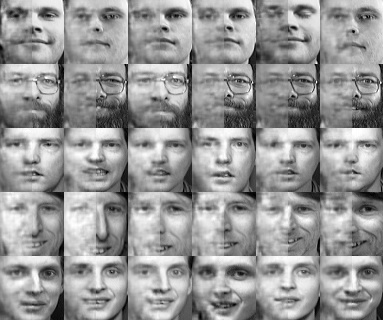
\includegraphics[width=0.35\textwidth]{completion.png}
  \caption{Example Olivetti test set image completions of the bundle entropy ICNN.}
  \label{fig:images-completed}
\end{figure}

\cref{table:image} shows the test MSEs for the different approaches
and example image completions are shown in \cref{fig:images-completed}.
We note that as future work, an ICNN variant of the baseline dilated
CNN and FCN architectures could be made in addition to
the DQN architecture the ICNN in this experiment uses.
For ICNNs, these results show that the bundle entropy method can
leverage more information from these five iterations than gradient
descent, even when the convexity constraint is relaxed.
The PICNN trained with back-optimization with the relaxed convexity
constraint slightly outperforms the network with
the convexity constraint, but not the network trained with the
bundle-entropy method.
This shows that for image completion with PICNNs, convexity does not
seem to inhibit the representational power.
Furthermore, this experiment suggests that a small number of
inner optimization iterations (five in this case) is
sufficient for good performance.

\begin{table}
\begin{center}
\begin{tabular}{@{}ll@{}}
Method & MSE \\ \hline
Sum-Product Network Baseline \citep{poon2011sum} & 942.0 \\
Dilated CNN Baseline \citep{yu2015multi} & 800.0 \\
FCN Baseline \citep{long2015fully} & \textbf{795.4} \\ \hline
ICNN - Bundle Entropy & 833.0 \\
ICNN - Gradient Decent & 872.0 \\
ICNN - Nonconvex & 850.9 \\
\end{tabular}
\caption{Olivetti image completion test reconstruction errors.}
\label{table:image}
\end{center}
\end{table}

\subsection{Continuous Action Reinforcement Learning}
Finally, we present standard benchmarks in continuous action reinforcement
learning from the OpenAI Gym \citep{brockman2016openai} that use the
MuJoCo physics simulator \citep{todorov2012mujoco}.
We consider the environments shown in \cref{tab:gym-szs}.
% $\mathcal {S} \times \mathcal{A}$,
We model the (negative) $Q$ function,
$-Q(s,a;\theta)$ as an ICNN and select actions with
the convex optimization problem
$a^\star(s) = \argmin_a -Q(s,a;\theta)$.
We use Q-learning to optimize the ICNN as described in
\cref{sec:icnn:learning} and
\cref{alg:icnn-rl}.
At test time, the policy is selected by optimizing $Q(s, a; \theta)$.
All of our experiments use a PICNN with two fully-connected
layers that each have 200 hidden units.
We compare to Deep Deterministic Policy Gradient (DDPG) \citep{lillicrap2015continuous}
and Normalized Advantage Functions (NAF) \citep{gu2016continuous}
as state-of-the-art off-policy learning baselines.\footnote{Because there are
not official DDPG or NAF implementations or
results on the OpenAI gym tasks, we use the Simon Ramstedt's
DDPG implementation from \url{https://github.com/SimonRamstedt/ddpg}
and have re-implemented NAF.}

\begin{table}[H]
  \centering
  \begin{tabular}{rrr}
    Environment & \# State & \# Action \\ \hline
    InvertedPendulum-v1	& 4 & 1 \\
    InvertedDoublePendulum-v1	& 11 & 1 \\
    Reacher-v1	& 11 & 2 \\
    HalfCheetah-v1	& 17 & 6 \\
    Swimmer-v1	& 8 & 2 \\
    Hopper-v1	& 11 & 3 \\
    Walker2d-v1	& 17 & 6 \\ %\hline
    Ant-v1	& 111 & 8 \\
    Humanoid-v1	& 	376 & 17 \\
    HumanoidStandup-v1	& 	376 & 17 \\
  \end{tabular}
  \caption{State and action space sizes in the OpenAI gym MuJoCo benchmarks.}
  \label{tab:gym-szs}
\end{table}

\begin{algorithm}[H]
  \caption{Deep Q-learning with ICNNs.
    \texttt{Opt-Alg} is a convex minimization algorithm such as
    gradient descent or the bundle entropy method.
    $\tilde Q_\theta$ is the objective the optimization algorithm solves.
    In gradient descent, $\tilde Q_\theta(s,a) = Q(s, a|\theta)$ and
    with the bundle entropy method, $\tilde Q_\theta(s,a) = Q(s, a|\theta) + H(a)$.
  }
  \begin{algorithmic}
    \State{Select a discount factor $\gamma\in(0,1)$ and moving average factor
      $\tau\in(0,1)$}
    \State{Initialize the ICNN $-Q(s, a|\theta)$ with
      target network parameters $\theta'\leftarrow\theta$
      and a replay buffer $R\leftarrow\emptyset$}
    % \Let{$\theta'$}{$\theta$}\Comment{Initialize the target network parameters.}
    \For{each episode $e=1,E$}
    \State{Initialize a random process $\mathcal{N}$ for action exploration}
    \State{Receive initial observation state $s_1$}
    \For{$i=1,I$}
    \Let{$a_i$}{\Call{Opt-Alg}{$-Q_\theta$, $s_i$, $a_{i,0}$}+$\mathcal{N}_i$}
    \Comment{For some initial action $a_{i,0}$}
    % \State{Select action $a_i=bundle\_entropy(f, \partial{f} | \theta)+\mathcal{N}_i$}
    \State{Execute $a_i$ and observe $r_{i+1}$ and $s_{i+1}$}
    \State \Call{Insert}{$R$, $(s_i, a_i, s_{i+1}, r_{i+1})$}
    \State{Sample a random minibatch from the replay buffer: $R_M\subseteq R$}
    \For{$(s_m, a_m, s_m^+, r_m^+)\in R_M$}
    \Let{$a_m^+$}{\Call{Opt-Alg}{$-Q_{\theta'}$,$s_{m}^+$,$a_{m,0}^+$}}
    \Comment{Uses the target parameters $\theta'$}
    \Let{$y_m$}{$r_m^+ + \gamma Q(s_m^+, a_m^+|\theta')$}
    \EndFor
    \State{Update $\theta$ with a gradient step to minimize
      $\mathcal{L} = \frac{1}{|R_M|}\sum_m\big(\tilde Q(s_m, a_m|\theta)-y_m\big)^2$}
    \Let{$\theta'$}{$\tau\theta + (1-\tau)\theta'$}
    \Comment{Update the target network.}
    \EndFor
    \EndFor
  \end{algorithmic}
  \label{alg:icnn-rl}
\end{algorithm}

\begin{table}
\begin{center}
\begin{tabular}[c]{@{}llll@{}}
Task & DDPG & NAF & ICNN \\ \hline
Ant & 1000.00 & 999.03 & \textbf{1056.29} \\
HalfCheetah & 2909.77 & 2575.16 & \textbf{3822.99} \\
Hopper & \textbf{1501.33} & 1100.43 & 831.00 \\
Humanoid & 524.09 & \textbf{5000.68} & 433.38 \\
HumanoidStandup & 134265.96 & 116399.05 & \textbf{141217.38} \\
InvDoubPend & \textbf{9358.81} & \textbf{9359.59} & \textbf{9359.41} \\
InvPend & \textbf{1000.00} & \textbf{1000.00} & \textbf{1000.00} \\
Reacher & -6.10 & -6.31 & \textbf{-5.08} \\
Swimmer & 49.79 & \textbf{69.71} & 64.89 \\
Walker2d & \textbf{1604.18} & 1007.25 & 298.21 \\
\end{tabular}

\caption{Maximum test reward for ICNN algorithm versus alternatives on several
OpenAI Gym tasks. (All tasks are v1.)}
\label{tab:rl:maxTestRew}
\end{center}
\end{table}

\cref{tab:rl:maxTestRew} shows the maximum test reward achieved
on these tasks and, shows the ICNNs \emph{can} be used as a
drop-in replacement for a function approximator in Q-learning.
Comparing the performance of the algorithms does not give
a clear winner, as no algorithm strictly outperforms the others
and there are non-deterministic and high-variance issues
in evaluating deep RL agents \citep{henderson2018deep}.

NAF poses a particularly interesting comparison point to ICNNs.
In particular, NAF decomposes the $Q$ function in terms of the
value function an an advantage function
$Q(s,a) = V(s) + A(s,a)$ where the advantage function is restricted to
be \emph{concave quadratic} in the actions, and thus always has a closed-form
solution.  In a sense, this closely mirrors the setup of the PICNN architecture:
like NAF, we have a separate non-convex path for the $s$ variables, and an
overall function that is convex in $a$; however, the distinction is that while
NAF requires that the convex portion be quadratic, the ICNN
architecture allows any convex functional form.

\section{Conclusion and future work}
This chapter laid the groundwork for the input convex neural network model.  By
incorporating relatively simple constraints into existing network architectures,
we can fit very general convex functions and the apply optimization as an
inference procedure.  Since many existing models already fit into this overall
framework (e.g., CRF models perform an optimization over an output space where
parameters are given by the output of a neural network), the proposed method
presents an extension where the entire inference procedure is ``learned'' along
with the network itself, without the need for explicitly building typical
structured prediction architectures.  This work explored only a small subset of
the possible applications of these network, and the networks offer promising
directions for many additional domains.

%%% Local Variables:
%%% coding: utf-8
%%% mode: latex
%%% TeX-engine: xetex
%%% TeX-master: "../thesis"
%%% End:


\part{Extensions and Applications}
\graphicspath{{cvxpyth/}}

\chapter{Differentiable \cvxpy Optimization Layers}
\label{sec:cvxpyth}

In this chapter, we show how to turn the \cvxpy
modeling language \citep{diamond2016cvxpy} into
a differentiable optimization layer and
implement our method in PyTorch \citep{paszke2017automatic}.
This allows users to express convex optimization layers in
the intuitive \cvxpy modeling language without needing
to manually implement the backward pass.

\section{Introduction}
This thesis has presented differentiable optimization layers
as a powerful class of operations for end-to-end learning
that allow more specialized domain knowledge to be integrated
into the modeling pipeline in a differentiable way.
Convex optimization layers can be represented as
\begin{equation}
  \label{eq:optimization-layer}
  z_{i+1} = \argmin_z f_\theta(z, z_i)\;
  {\rm s.t.}\;z\in \CC_\theta(z_i)
\end{equation}
where $z_i$ is the previous layer,
$f$ is a convex objective function parameterized
by $\theta$, and $\CC$ is a convex constraint set.
From the perspective of end-to-end learning,
convex optimization layers can be seen
as a module that outputs $z_{i+1}$ and has parameters
$\theta$ that can be learned with gradient descent.
We note that the convex case captures many
of the applications above, and can be used as
a building block for differentiable non-convex
optimization problems.

Implementing optimization layers can be non-trivial as explicit
closed-form solutions typically do not exist.
The forward pass needs to call into an optimization
problem solver and the backward pass typically
\emph{cannot} leverage automatic differentiation.
The backwards pass is usually implemented by implicitly
differentiating the KKT conditions of the optimization problem
as done in bilevel optimization
\citep{gould2016differentiating,kunisch2013bilevel},
sensitivity analysis
\citep{bertsekas1999nonlinear,fiacco1990sensitivity,bonnans2013perturbation},
and in our OptNet approach \cref{sec:optnet}.
Thus to implement an optimization layer, users
have to manually implement the backwards pass,
which is cumbersome and error-prone,
or use an existing optimization problem layer such as
the differentiable QP layer from \cref{sec:optnet},
which is not capable of exploiting problem-specific
structures, uses dense operations, and requires
the user to manually transform their problem into
a standard form.

We make \cvxpy differentiable with respect to the
\texttt{Parameter} objects provided to the optimization problem
by making internal \cvxpy components differentiable.
This involves differentiating the reduction from the \cvxpy
language to the problem data of a cone program in standard form
and then differentiating through the cone program.
We show how to differentiate through cone programs by
implicitly differentiating the residual map from
\citet{busseti2018solution},
which is of standalone interest as
this shows how to differentiate through optimization
problems with non-polytope constraints.

\section{Background}
\subsection{The \cvxpy modeling language}
\label{sec:bg:cvxpy}
\cvxpy \citep{diamond2016cvxpy}
is a domain-specific modeling language
based on disciplined convex programming
\citep{grant2006disciplined}
that allows users to express optimization problems
in a more natural way than the standard form
required my most optimization problem solvers.
\cvxpy works by transforming the optimization
problem from their domain-specific language to a
standard (or canonical) form that is passed into
a solver. This inner canonicalized problem is
then solved and the results are returned to
the user. In this chapter, we focus on the
canonicalization to a cone program, which is
one of the most commonly used modes as most convex
optimization problems can be expressed as a cone program,
although we note that our method can be
applied to other \cvxpy solvers.
\cref{fig:overview} overviews the relevant
\cvxpy components.

\subsection{Cone Preliminaries}
A set $\mathcal{K}$ is a \emph{cone}
if for all $x\in\mathcal{K}$ and $t>0$,
$tx\in\mathcal{K}$.
The \emph{dual cone} of a cone $\mathcal{K}$ is
$$\mathcal{K}^* =\menge{y}{\inf_{x\in \mathcal{K}} y^\top x\ge 0}.$$
Commonly used cones include the
nonnegative orthant $\menge{x}{x\geq 0}$,
second-order cone $\menge{(x,t)\in\RR^n_+}{t\geq ||x||_2}$,
positive semidefinite cone $\{X=X^\top \succeq 0\}$,
and
exponential cone
\begin{equation}
  \menge{(x,y,z)}{y>0, ye^{x/y} \leq z} \cup
  \menge{(x,0,z)}{x\leq 0, z\geq 0}
\end{equation}
We can also create a cone from the Cartesian
products of simpler cones as
$\mathcal{K}=\mathcal{K}_1\times \ldots \times\mathcal{K}_p$.

\subsection{Cone Programming}
Most convex optimization problems can be represented and
efficiently solved as a cone program that uses
the nonnegative orthant, second-order cone,
positive semidefinite cone, and exponential cones.
This applicability makes them a commonly used internal
solver for \cvxpy, which implements many of the
well-known transformations from problems to their
conic form.
In the following we state properties of cone programs
and useful definitions for this chapter.
More details about cone programming can be found in
\citet{boyd2004convex,ben2001lectures,busseti2018solution,odonoghue2016conic,lobo1998applications,alizadeh2003second}.

In their primal (P) and dual (D) forms,
cone programs can be represented as \\
\begin{minipage}{0.45\textwidth}
  \begin{equation*}
    % \tag{P}
    \begin{array}{lll}
      \text{(P)}\;\; \xstar, \sstar =
      &\argmin_{x,s} &c^\top x\\
      &\subjectto &  Ax+s=b\\
      &  &s\in  \mathcal{K}
    \end{array}
  \end{equation*}
  \vspace{3mm}
\end{minipage}
\hfill
\begin{minipage}{0.5\textwidth}
  \begin{equation}
    \label{eq:cp}
    % \tag{D}
    \begin{array}{lll}
      \text{(D)}\;\; \ystar =
      & \argmax_y & b^\top y\\
      &\subjectto & A^\top y+c=0\\
      &&y\in  \mathcal{K}^*
    \end{array}
  \end{equation}
  \vspace{3mm}
\end{minipage}
where $x\in\R^n$ is the \emph{primal variable},
$s\in\R^m$ is the \emph{primal slack variable},
$y\in\R^m$ is the \emph{dual variable}.
and $\mathcal{K}$ is a nonempty, closed, convex cone
with dual cone $\mathcal{K}^*$.

\textbf{The KKT optimality conditions.}
The Karush--Kuhn--Tucker (KKT) conditions for the
cone program in \cref{eq:cp} provide
necessary and sufficient conditions for optimality
and are defined by
\begin{equation}
\label{eq:cp-kkt}
Ax +s =b, \quad
A^\top y + c = 0, \quad
s \in \mathcal{K}, \quad
y \in \mathcal{K}^*, \quad
s^\top y = 0.
\end{equation}
The complimentary slackness condition $s^\top y = 0$ can
alternatively be captured with a condition that
makes the duality gap zero $c^\top x + b^\top y = 0$.

\textbf{The homogenous self-dual embedding.}
\citet{ye1994nl} converts the primal and cone dual programs
in \cref{eq:cp} into a single feasibility problem called
the homogenous self-dual embedding, which is defined by
\begin{equation}
\label{e:hsde:1}
Qu = v, \quad u \in \mathbfcal{K},
\quad v \in \mathbfcal{K}^*, \quad u_{m+n+1} +
 v_{m+n+1} >0,
\end{equation}
where
\[
\mathbfcal{K} = \RR^n \times \mathcal{K}^*\times \RR_+, \quad
\mathbfcal{K}^* = \{0\}^n\times \mathcal{K}\times \RR_+,
\]
and $Q$ is the skew-symmetric matrix
\[
	Q = \begin{bmatrix}
		0 & A{^\top} & c\\
		-A & 0 & b \\
		-c{^\top} & -b{^\top} & 0
	\end{bmatrix}.
\]
A solution to this embedding problem $(\ustar, \vstar)$
can be used to determine the solution of a conic
problem, or to certify the infeasibilty of the
problem if a solution doesn't exist.
If a solution exists, then
$\ustar=(\xstar/\tau,\ystar/\tau,\tau)$
and
$\vstar=(0, \sstar/\tau, 0)$.

\textbf{The conic complementarity set.}
The \emph{conic complementarity set} is defined by
\begin{equation}
\label{eq:con:com:set}
\mathcal{C} = \menge{(u,v) \in
  \mathbfcal{K} \times \mathbfcal{K}^* }{u^\top v = 0}.
\end{equation}
We denote
the Euclidean projection onto
$\mathbfcal{K}$ with $\Pi$
and
the Euclidean projection onto
$-\mathbfcal{K}^*$ with $\Pi^*$.
\citet{moreau1961decomposition} shows that
$\Pi^*=I-\Pi$.

\textbf{Minty's parameterization of the complementarity set.}
Minty's parameterization $M: \RR^{m+n+1} \to \mathcal{C}$
of $\mathcal{C}$ is defined by
$M(z) = (\Pi z, -\Pi^* z)$.
This parameterization is invertible with
$M^{-1}(u,v) = u-v$.
See
\citet[Corollary~31.5.1]{rockafellar1970convex}
and \citet[Remark~23.23(i)]{bauschke2017convex}
for more details.
The homogeneous self-dual embedding can be expressed
using Minty's parameterization as
$-\Pi^* z=Q\Pi z$ where $z_{m+n+1} \neq 0$.

\textbf{The residual map of Minty's parameterization.}
\label{sec-residual-map}
\citet{busseti2018solution} defines the
\emph{residual map} of Minty's parameterization
$\Res: \RR^{m+n+1}\to \RR^{m+n+1}$
as
\begin{equation}
\label{eq-residual}
\Res(z) = Q\Pi z+\Pi^*z=((Q-I)\Pi+I)z.
\end{equation}
and shows how to compute the derivative of it
when $\Pi$ is differentiable at $z$ as
\begin{equation}
\label{eq:res:der}
\DD_z\Res(z) =(Q-I)\DD_z\Pi(z) +I,
\end{equation}
where $z\in \RR^{m+n+1}$.
The cone projection differentiation $\DD_z \Pi(z)$
can be computed as described in
\citet{ali2017semismooth}.

\textbf{The Splitting Conic Solver (SCS).}
SCS \citep{odonoghue2016conic} is an efficient way of solving
general cone programs by using the alternating
direction method of multipliers (ADMM)
\citep{boyd2011distributed} and is a commonly used
solver with \cvxpy.
In the simplified form, each iteration
of SCS consists of the following three steps:
\begin{equation}
\begin{array}{rcl}
\tilde u^{k+1} &=& (I + Q)^{-1} (u^k + v^k )\\[1ex]
u^{k+1} &=& \Pi\left(\tilde u^{k+1} - v^k\right) \\[1ex]
v^{k+1} &=&  v^k - \tilde u^{k+1} + u^{k+1}.
\end{array}
\label{eq:scs}
\end{equation}

The first step projects onto an affine subspace,
the second projects onto the cone
and the last updates the dual variable.
In this paper we will mostly focus on solving the
affine subspace projection step. \citet[Section 4.1]{odonoghue2016conic}
shows that the affine subspace projection can be
reduced to solving linear systems of the form
\begin{equation}
\label{eq:scs-linsys}
\begin{bmatrix}
I & -A^\top \\
-A & -I  \\
\end{bmatrix}
\begin{bmatrix} z_x \\ -z_y \end{bmatrix}
=
\begin{bmatrix} w_x \\ w_y \end{bmatrix},
\end{equation}
which can be re-written as
\begin{equation}
  \label{eq:scs-linsys-elim}
  z_x = (I + A^\top A)^{-1}(w_x - A^\top w_y), \quad
  z_y = w_y + A z_x.
\end{equation}

\section{Differentiating \cvxpy and Cone Programs}
\label{sec:cvxpyth:diff-cp}

\begin{figure}[t]
  \centering
  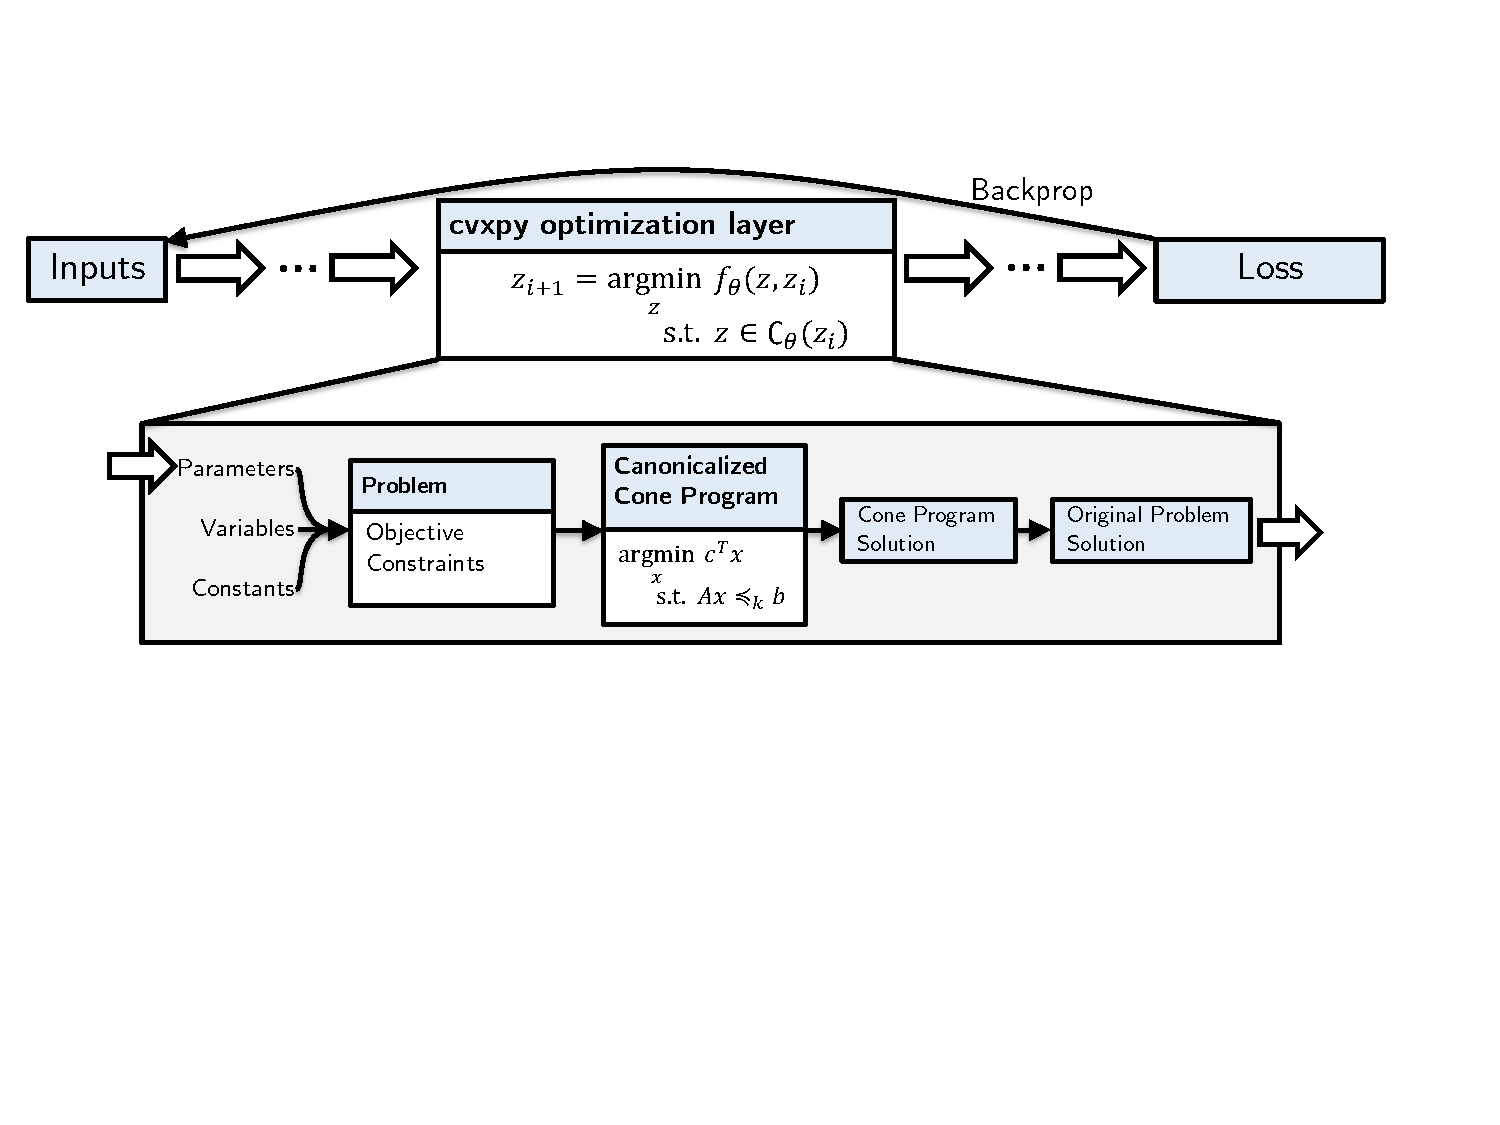
\includegraphics[width=0.9\textwidth]{overview.pdf}
  \caption{
    Summary of our differentiable \cvxpy layer that allows
    users to easily turn most convex optimization problems into
    layers for end-to-end machine learning.
  }
  \label{fig:overview}
\end{figure}

We have created a differentiable \cvxpy layer
by making the relevant components differentiable,
which we visually show in \cref{fig:overview}.
We make the transformation from the problem data in the original
form to the problem data of the canonicalized cone problem
differentiable by replacing the numpy operations for this component
with PyTorch \citep{paszke2017automatic} operations.
We then pass this data into a differentiable cone program
solver, which we show how to create in \cref{sec:diff-cp}
by implicitly differentiating the residual map of
Minty's parameterization for the backward pass.
The solution of this cone program can then be mapped
back up to the original problem space in a differentiable
way and returned.

\subsection{Differentiating Cone Programs}
\label{sec:diff-cp}
We consider the argmin of the primal cone program
in \cref{eq:cp} as a function that maps from the
problem data $\theta = \{c, A, b\}$ to the solution $\xstar$.
The approach from \cref{sec:optnet}
that differentiates through convex quadratic programs by
implicitly differentiating the KKT conditions
is difficult to use for cone programs.
This is because the cone constraints in the KKT conditions
in \cref{eq:cp-kkt} make it difficult to form a
set of implicit functions.
Instead of implicitly differentiating the KKT conditions,
we show how to similarly apply implicit
differentiation to the residual map of
Minty's parameterization shown in \citet{busseti2018solution}
to compute the derivative
$\partial \xstar/\partial \theta$.
Furthermore for backpropagation, the full Jacobian is
expensive and unnecessary to form and we show how to
efficiently compute $\partial \ell/\partial \theta$
given $\partial \ell/\partial \xstar$.

\subsubsection{Implicit differentiation of the residual map}
We assume that we have solved the forward pass of the
cone program in \cref{eq:cp} and have a solution
$\xstar, \sstar, \ystar$.
We now show how to compute
$\partial \xstar/\partial \theta$.
This derivation was concurrently considered and done by
\citet{agrawal2019differentiating}.

We construct $\ustar=(\xstar, \ystar, 1)$,
and $\vstar=(0,\sstar, 0)$, and $\zstar=\ustar-\vstar$.
The residual map of Minty's parameterization is zero,
$R(\zstar)=0$, and forms a set of
implicit equations that describe the solution mapping.
Implicit differentiation can be done as described in
\citet{dontchev2009implicit} with
\begin{equation}
  \label{eq:residual-implicit-diff}
  \DD_\theta \zstar =
    -\left(\DD_z \Res(\zstar)\right)^{-1}
    \DD_\theta \Res(\zstar).
\end{equation}
$\left(\DD_z \Res(\zstar)\right)^{-1}$ can be computed
as described in \citep{busseti2018solution}
and $\DD_\theta \Res(\zstar)$ can be analytically computed.
We consider the scaling factor $\tau=z_{m+n+1}=1$ to be
a constant because a solution to the cone program exists.
Finally, applying the chain rule to $\ustar=\Pi \zstar$
gives
\begin{equation}
  \DD_\theta \ustar = (\DD_z \Pi z) \DD_\theta \zstar.
\end{equation}
We note that implicitly differentiating the residual
map captures implicit differentiation of the KKT conditions
as a special case for simple cones such as the zero cone
and non-negative orthant.

The linear system in \cref{eq:residual-implicit-diff}
can be expensive to solve.
In special cases such as quadratic programs and LQR problems
that we discussed in \cref{sec:optnet} and
\cref{sec:empc}, respectively, this system can be interpreted
as the solution to another convex optimization problem
and efficiently solved with a method similar to the
forward pass.
This connection is made by interpreting the linear system
solve as a KKT system solve that represents another
optimization problem.
However for general cone programs it is more difficult
to interpret this linear system as a KKT system
because of the cone projections and therefore it
is more difficult to interpret this linear system
solve as an optimization problem.

\section{Implementation}
\subsection{Forward Pass: Efficiently solving batches of
  cone programs with SCS and PyTorch}
\label{sec:cp:efficient}

Na\"ively implemented optimization layers can become
computational bottlenecks when used in a machine learning
pipeline that requires efficiently processing
minibatches of data.
This is because most other parts of the modeling pipeline
involve operations such as linear maps, convolutions,
and activation functions that can quickly be executed
on the GPU to exploit data parallelism across the minibatch.
Most off-the-shelf optimization problem solvers are designed for
the setting of solving a single problem at a time and are not easily
able to be plugged into the batched setting required
when using optimization layers.

To overcome the computational challenges of solving batches
of cone programs concurrently, we have created a batched
PyTorch and potentially GPU-backed backend for the
Splitting Conic Solver (SCS) \citep{odonoghue2016conic}.
The bottleneck of the SCS iterates in \cref{eq:scs}
is typically in the subspace projection part that solves
linear systems of the form
\begin{equation}
  \tilde u^{k+1} = (I + Q)^{-1} (u^k + v^k )
\end{equation}
We have added a new linear system solver backend to the
official SCS C implementation that calls back
up into Python to solve this linear system.

Our cone program layer implementation offers the following
modes for solving a batch of $N$ cone programs
represented in standard form as in \cref{eq:cp} with
as $\theta_i=\{A_i, b_i, c_i\}$
for $i\in\{1, \ldots, N\}$ with SCS.
As common in practice, we assume that the cone programs
have the structure and use the same cones but have
different problem data $\theta_i$.
We empirically compare these modes in \cref{sec:eval}.

\paragraph{Vanilla SCS, serialized.}
This is a baseline mode that is the easiest to implement and sequentially
iterates through the problems $\theta_i$.
This lets us use the vanilla SCS sparse direct and indirect
linear system solvers on the CPU and CUDA, but does
not take advantage of data parallelism.

\paragraph{Vanilla SCS, batched.}
This is another baseline mode that comes from observing that a
batch of cone programs can be represented as
a single cone program in standard form as in \cref{eq:cp} with
variables $x=[x_1^\top, \ldots, x_N^\top]^\top$
and data $A=\mathrm{diag}(A_1, \ldots, A_N)$,
$b=[b_1^\top, \ldots, b_N^\top]^\top$,
and $c=[c_1^\top, \ldots, c_N^\top]^\top$.
This exploits the knowledge that all of the cone programs
can be solved concurrently. The bottleneck of this
mode is still typically in the linear system solve
portion of SCS, which happens using sparse operations
on the CPU or GPU.

\paragraph{SCS+PyTorch, batched.}
In this mode we represent the batch of cone programs as a single
batched cone program use SCS will callbacks up into Python so
that we can use PyTorch to efficiently solve the linear system.
This allows us to keep the $A$ data in PyTorch and potentially
on the GPU without converting/transferring it and passing it
into the SCS.
Specifically we use dense operations and have implemented
direct and indirect methods to solve \cref{eq:scs-linsys-elim}
in PyTorch and then pass the result back down into SCS for the
rest of the operations.
Our direct method uses PyTorch's batched LU factorizations and
solves and our indirect method uses a batched conjugate
gradient (CG) implementation.
These custom linear system solvers are able to explicitly take
advantage of the independence present in the linear systems
that the sparse linear system solvers may not recognize automatically,
and the dense solvers are also useful for dense cone programs,
which come up in the context of differentiable optimization
layers when large portions of the constraints are being learned.

\subsection{Backward pass: Efficiently solving the linear system}
When using cone programs as layers in end-to-end learning systems
with some scalar-valued loss function $\ell$,
the full Jacobian $\DD_\theta \xstar$ is expensive
and unnecessary to form and requires solving
$|\theta|$ linear systems.
The Jacobian is only used when applying the chain rule
to obtain $\DD_\theta \ell = (\DD_\xstar\ell) \DD_\theta \xstar$.
We can directly compute $\DD_\theta \ell$ without computing
the intermediate Jacobian by solving a single linear system.
Following the method of \cref{sec:optnet}, we set up the system
\begin{equation}
  \label{eq:cvxpyth:diff_efficient}
  \DD_z \Res(\zstar)
\begin{bmatrix}
  d_{z_1} \\
  d_{z_2} \\
  0 \\
\end{bmatrix} = \\
-
\begin{bmatrix}
  \nabla_\xstar \ell \\
  0 \\
  0 \\
\end{bmatrix}.
\end{equation}
Applying the chain rule to $\ustar=\Pi \zstar$ gives
$d_x = d_{z_1}$ and
$d_y = (\DD_z \Pi z) d_{z_2}$.
We then compute the relevant backpropagation derivatives as
\begin{equation}
  \nabla_c \ell = d_x
  \hspace{20mm}
  \nabla_A \ell = d_y \otimes \xstar + \ystar \otimes d_x
  \hspace{20mm}
  \nabla_b \ell = -d_y
\end{equation}

Solving \cref{eq:cvxpyth:diff_efficient} is still challenging
to implement in practice as $\DD_z \Res(\zstar)$ can be large
and sparse and doesn't have obviously exploitable properties such
as symmetry or anti-symmetry.
In addition to directly solving this linear system, we
also explore the use of LSQR \citep{paige1982lsqr} as an
iterative indirect method of solving this system
in \cref{sec:cvxpyth:bw_prof}.
Our LSQR implementation uses the implementation from
\citet{ali2017semismooth} to compute $\DD_z \Pi(z)$
in the form of an abstract linear operator so the
full matrix does not need to be explicitly formed.

\newpage
\section{Examples}
\label{sec:cvxpyth:examples}

This section provides example use cases of our \cvxpy
optimization layer. All of these use the preamble

\begin{lstlisting}
import cvxpy as cp
from cvxpyth import CvxpyLayer
\end{lstlisting}

\subsection{The ReLU, sigmoid, and softmax}
We will start with basic examples and revisit the optimization
views of the ReLU, sigmoid, and softmax from \cref{sec:bg:existing}.
These can be implemented with our \cvxpy layer
in a few lines of code.

\textbf{The ReLU.}
Recall from \cref{eq:relu-proj} that the optimization view is
\begin{equation*}
  f(x) = \argmin_y \;\; \frac{1}{2}||x-y||_2^2 \;\; \st \;\; y\geq 0.
\end{equation*}
We can implement this layer with:
\begin{lstlisting}
x = cp.Parameter(n)
y = cp.Variable(n)
obj = cp.Minimize(cp.sum_squares(y-x))
cons = [y >= 0]
prob = cp.Problem(obj, cons)
layer = CvxpyLayer(prob, params=[x], out_vars=[y])
\end{lstlisting}

This layer can be used and differentiated through
just as any other PyTorch layer.
Here is the output and derivative for a single
dimension, illustrating that this is indeed performing
the same operation as the ReLU.

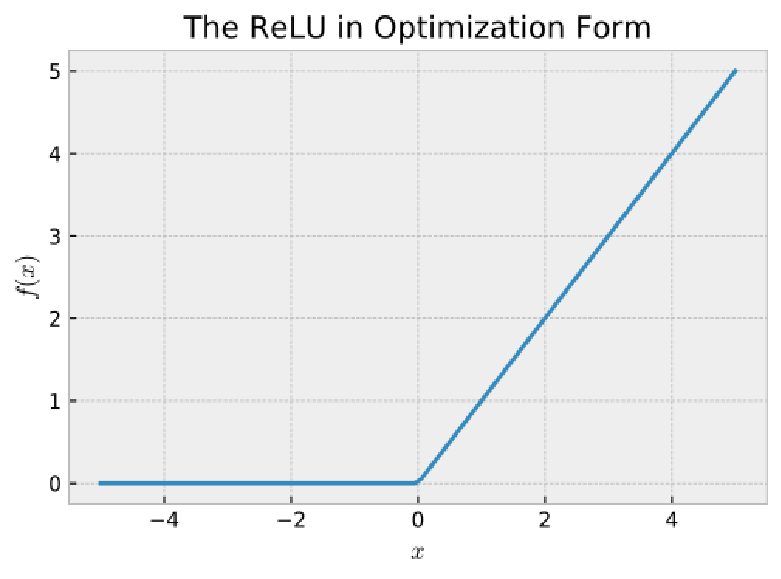
\includegraphics[height=2in]{fs/output_2.pdf}
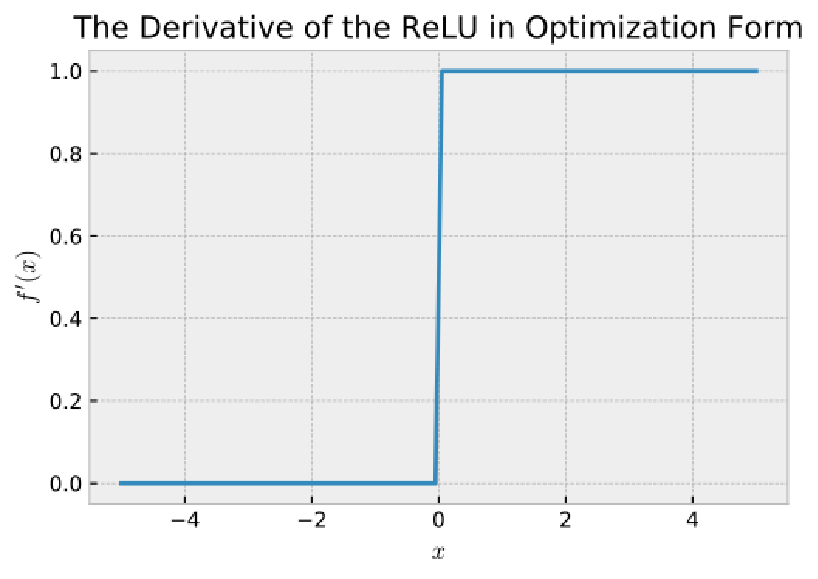
\includegraphics[height=2in]{fs/output_3.pdf}

\newpage
\textbf{The sigmoid.}
Recall from \cref{eq:sigmoid-proj} that the optimization view is
\begin{equation*}
f(x) = \argmin_{0<y<1} \;\; -x^\top y -H_b(y).
\end{equation*}
We can implement this layer with:
\begin{lstlisting}
x = cp.Parameter(n)
y = cp.Variable(n)
obj = cp.Minimize(-x.T*y - cp.sum(cp.entr(y) + cp.entr(1.-y)))
prob = cp.Problem(obj)
layer = CvxpyLayer(prob, params=[x], out_vars=[y])
\end{lstlisting}
We can also check that the output and derivative matches
what we expect from the usual sigmoid function:

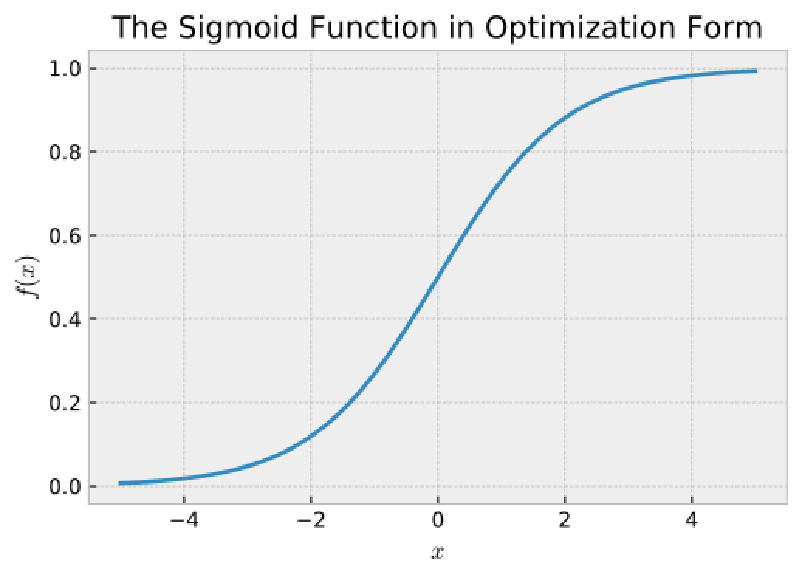
\includegraphics[height=2in]{fs/output_6.pdf}
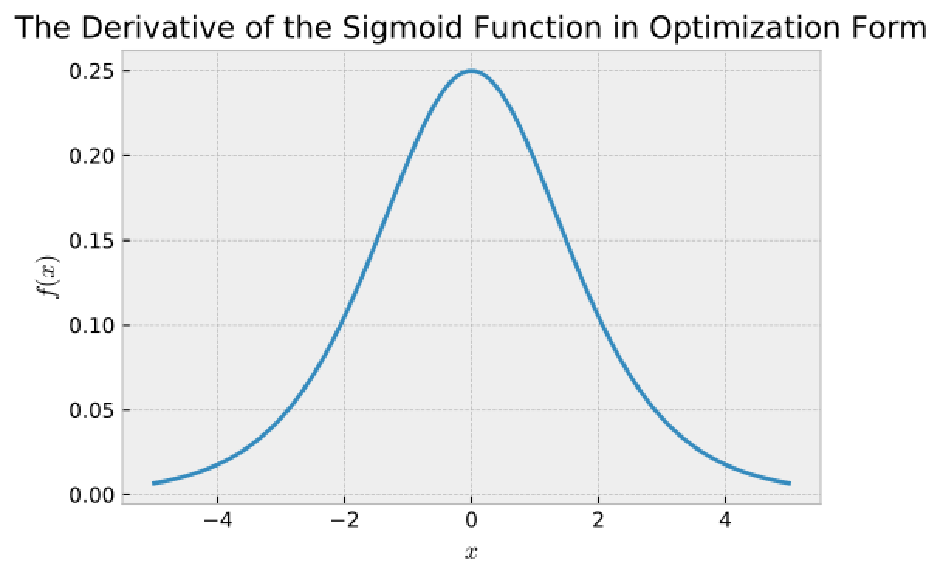
\includegraphics[height=2in]{fs/output_7.pdf}

\textbf{The softmax.}
Lastly recall from \cref{eq:simplex-proj} that the optimization view is
\begin{equation*}
f(x) = \argmin_{0<y<1} \;\; -x^\top y - H(y) \;\; \st\;\; 1^\top y = 1
\end{equation*}
We can implement this layer with:
\begin{lstlisting}
x = cp.Parameter(d)
y = cp.Variable(d)
obj = cp.Minimize(-x.T*y - cp.sum(cp.entr(y)))
cons = [sum(y) == 1.]
prob = cp.Problem(obj, cons)
layer = CvxpyLayer(prob, params=[x], out_vars=[y])
\end{lstlisting}

\newpage
\subsection{The OptNet QP}
We can re-implement the OptNet QP layer from \cref{sec:optnet}
with our differentiable \cvxpy{} layer in a few lines of code.
The OptNet layer is represented as a convex quadratic program
of the form
\begin{equation}
\begin{split}
x^\star = \argmin_{x} \;\; & \frac{1} {2}x^\top Qx + p^\top x \\
\subjectto \;\; & Ax = b \\
& Gx \leq h \\
\end{split}
\label{eq:cvxpy-qp}
\end{equation}
where $x \in \mathbb{R}^n$ is our optimization variable
$Q \in \mathbb {R}^{n \times n} \succeq 0$
(a positive semidefinite matrix),
$p \in \mathbb {R}^n$,
$A\in \mathbb{R}^{m \times n}$,
$b \in \mathbb{R}^m$,
$G \in \mathbb{R}^ {p \times n}$ and
$h \in \mathbb{R}^{p}$ are problem data.
We can implement this with:

\begin{lstlisting}
Q = cp.Parameter((n, n), PSD=True)
p = cp.Parameter(n)
A = cp.Parameter((m, n))
b = cp.Parameter(m)
G = cp.Parameter((p, n))
h = cp.Parameter(p)
x = cp.Variable(n)
obj = cp.Minimize(0.5*cp.quad_form(x, Q) + p.T * x)
cons = [A*x == b, G*x <= h]
prob = cp.Problem(obj, cons)
layer = CvxpyLayer(prob, params=[Q, p, A, b, G, h], out=[x])
\end{lstlisting}

This layer can then be used by passing in the
relevant parameter values:
\begin{lstlisting}
Lval = torch.randn(nx, nx, requires_grad=True)
Qval = Lval.t().mm(Lval)
pval = torch.randn(nx, requires_grad=True)
Aval = torch.randn(ncon_eq, nx, requires_grad=True)
bval = torch.randn(ncon_eq, requires_grad=True)
Gval = torch.randn(ncon_ineq, nx, requires_grad=True)
hval = torch.randn(ncon_ineq, requires_grad=True)
y = layer(Qval, pval, Aval, bval, Gval, hval)
\end{lstlisting}

\newpage
\subsection{Learning Polyhedral Constraints}
We demonstrate how gradient-based learning can be done with
a \cvxpy layer in this synthetic example.
Consider the polyhedrally constrained
projection problem
\begin{align*}
\hat y = \argmin_y\;\; &\frac{1}{2}||p-y||_2^2  \\
 {\rm s.t.}\;\; & Gy\leq h \\
\end{align*}
Suppose we don't know the polytope's parameters $\theta=\{G, h\}$
and want to learn them from data.
Then using the MSE for $\ell$, we can randomly initialize
ellipsoids $\theta$ and learn them with gradient steps $\nabla_\theta \ell$.
We note that this problem is meant for illustrative purposes and
could be solved by taking the convex hull of the input data points.
However our approach would still work if this was over a latent
and unobserved part of the model, of if you want to take an
approximate convex hull that limits the number of polytope edges.

We can implement this layer with the following code.
\cref{fig:polytope-results} shows the results of learning
on two examples.
Each problem has a true known polytope that we show in blue
and the model's approximation is in red.
Learning starts on the left with randomly initialized
polytopes that are updated with gradient steps,
which are shown in the images progressing to the right.

\begin{lstlisting}
G = cp.Parameter((m, n))
h = cp.Parameter(m)
p = cp.Parameter(n)
y = cp.Variable(n)
obj = cp.Minimize(0.5*cp.sum_squares(y-p))
cons = [G*y <= h]
prob = cp.Problem(obj, cons)
layer = CvxpyLayer(prob, params=[p, G, h], out=[y])
\end{lstlisting}

\begin{figure}[t]
  \centering
  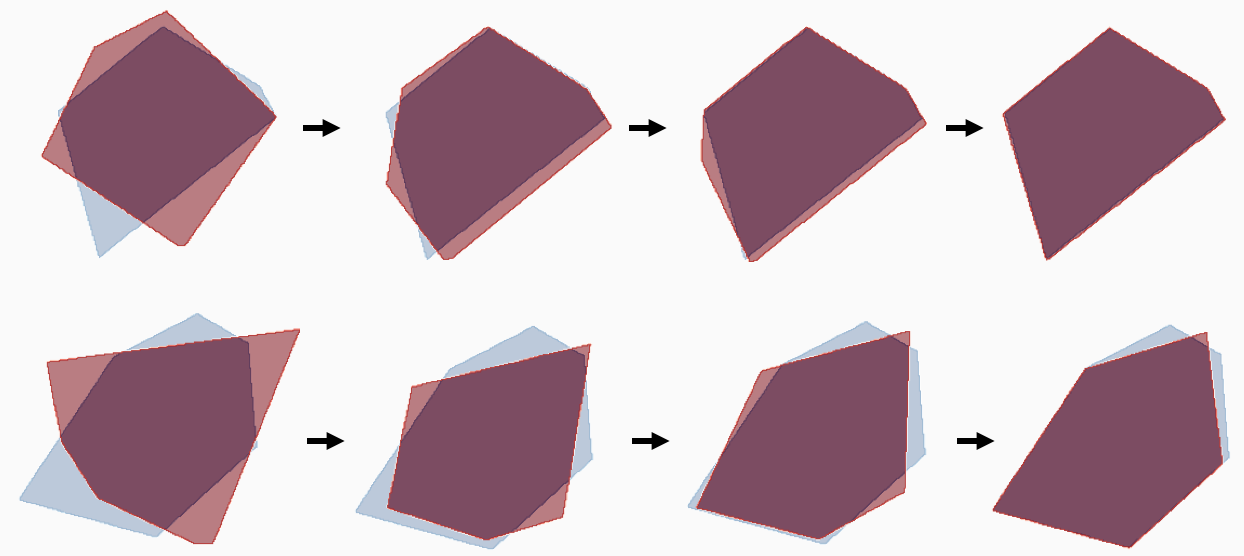
\includegraphics[width=0.6\textwidth]{polytope-frames.png} \\
  \cblock{190}{201}{216} True Polytope \enskip
  \cblock{176}{128}{131} Approximate Polytope
  \caption{
    Learning polyhedrally constrained problems.
  }
  \label{fig:polytope-results}
\end{figure}

\newpage
\subsection{Learning Ellipsoidal Constraints}
In addition to learning polyhedral constraints, we can easily
learn any parameterized convex constraint set.
Suppose instead that we want to learn an ellipsoidal
projection of the form
\begin{align*}
\hat y = \argmin_y\;\; &\frac{1}{2}||p-y||_2^2  \\
 {\rm s.t.}\;\; & \frac{1}{2}(y-z)^\top A(y-z) \leq 1
\end{align*}
with ellipsoid parameters $\theta=\{A,z\}$
This is an interesting optimization problem to consider because
it is an example of doing learning with a non-polytope
cone program (a SOCP), which prior approaches such as OptNet
could not easily handle.

We can implement this layer with the following code.
\cref{fig:ellipsoid-results} visualizes the learning process
on two examples.
As before, each problem has a true known ellipsoid that we show in blue
and the model's approximation is in red.
Learning starts on the left with randomly initialized
ellipsoids that are updated with gradient steps,
which are shown in the images progressing to the right.

\begin{lstlisting}
A = cp.Parameter((n, n), PSD=True)
z = cp.Parameter(n)
p = cp.Parameter(n)
y = cp.Variable(n)
obj = cp.Minimize(0.5*cp.sum_squares(y-p))
cons = [0.5*cp.quad_form(y-z, A) <= 1]
prob = cp.Problem(obj, cons)
layer = CvxpyLayer(prob, params=[p, A, z], out=[y])
\end{lstlisting}

\begin{figure}[t]
  \centering
  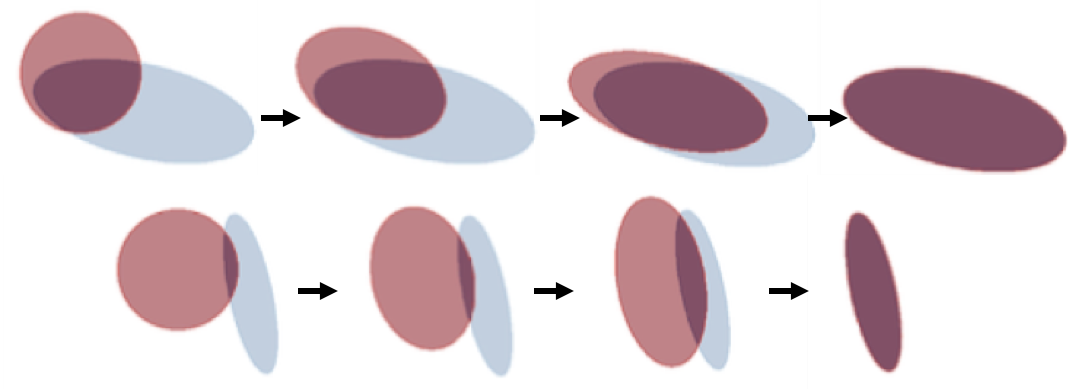
\includegraphics[width=0.6\textwidth]{ellipsoid-frames.png} \\
  \cblock{190}{201}{216} True Ellipsoid \enskip
  \cblock{176}{128}{131} Approximate Ellipsoid
  \caption{
    Learning ellipsoidally constrained problems.
  }
  \label{fig:ellipsoid-results}
\end{figure}

\newpage
\section{Evaluation}
\label{sec:eval}

In this section we analyze the runtime of our layer's forward
and backward passes compared to hand-written implementations
for commonly used optimization layers.
We will focus on three tasks:

\paragraph{Task 1: Dense QP.}
We consider a QP layer of the form
\cref{eq:cvxpy-qp} with a dense quadratic objective
and dense inequality constraints.
Our default experiment uses a QP with 100 latent
variables, 100 inequality constraints, and
a minibatch size of 128 examples.
We chose this task to understand how the performance
of our \cvxpy{} layer compares to the \qpth implementation
from \cref{sec:optnet}, which we use as a comparison point.
The problem size we consider here is comparable
to the QP problem sizes considered in \cref{sec:optnet}.
The backwards pass of \qpth is optimized to use a single
batched, pre-factorized linear system solve.

\paragraph{Task 2: Box QP.}
We consider a QP layer of the form
\cref{eq:cvxpy-qp} with a dense quadratic objective
constrained to the box $[-1, 1]^n$.
Our default experiment uses a QP with 100 latent
variables and a minibatch size of 128 examples.
We chose this task to study the impacts of
sparsity on the runtime.
We again use \qpth as the comparison point for these experiments.

\paragraph{Task 3: Linear Quadratic Regulator (LQR).}
We consider a continuous-state-action, discrete-time, finite-horizon
LQR problem of the form
\begin{equation}
  \label{eq:cvxpyth:lqr}
  \tau^{\star}_{1:T} = \argmin_{\tau_{1:T}}\;\;
  \sum_{t} \frac{1}{2} \tau_t^\top  C_t \tau_t + c_t^\top  \tau_t \;\;
  \subjectto\;\;
  x_1 = \xinit,\
  x_{t+1} = F_t\tau_t + f_t.
\end{equation}
where $\tau_{1:T} = \{x_t, u_t\}_{1:T}$ is the nominal trajectory,
$T$ is the horizon,
$x_t, u_t$ are the state and control at time $t$,
$\{C_t, c_t\}$ parameterize a convex quadratic cost,
and $\{F_t, f_t\}$ parameterize an affine system
transition dynamics.
We consider a control problem with 10 states,
2 actions, and a horizon of 5.
We compare to the differentiable model
predictive control (MPC) solver from
\citep{amos2018differentiable}, which uses batched
PyTorch operations to solve a batch of LQR problems with
the Riccati equations, and then implements the backward
pass with another, simpler, LQR solve with
the Riccati equations.

For each of these tasks we have measured the forward
and backward pass execution times for our layer in
comparison to the specialized solvers.
We have run these experiments on an unloaded system with
an NVIDIA GeForce GTX 1080 Ti GPU and
a four-core 2.60GHz Intel Xeon E5-2623 CPUs hyper-threaded
to eight cores.
We set the number of OpenMP threads to 8 for our experiments.
For numerical stability, we use 64-bits for all of
our implementations and baselines.
For \qpth and our implementation, we use an iteration
stopping condition of $\epsilon=10^{-3}$.

\newpage
\subsection{Forward pass profiling}
\cref{fig:eval:fwd} summarizes our main forward pass execution
times. \cref{fig:eval:fwd:all} shows the runtimes of all of the
modes and batch sizes, and \cref{fig:eval:fwd:speedups}
illustrates the speedup of our best mode compared to the
specialized solvers.
We have implemented and run every mode from \cref{sec:cp:efficient}
and our summary presents the best-performing mode,
which in every case on the GPU is our block direct solver.
On the CPU, serializing SCS calls is competitive for
problems with more sparsity.
For dense and sparse QPs on the CPU and GPU, our batched
SCS+PyTorch direct cone solver is faster than
the \qpth solver, which likely comes from the
acceleration, convergence, and normalization
tricks in SCS that are not present in \qpth.
The LQR task presents a sparse problem that illustrates
the challenges to using a general cone program formulation.
Our specialized solver that solves the Riccati equations in
batched form exploits the sparsity pattern of the problem
that is extremely difficult for the general cone program
formulation we consider here to take advantage of.
If the correct mappings to the cone program exist,
our layer could be modified to accept an
optimized user-provided solver for the forward pass
so that users can still take advantage of our backward
pass implementation.

\begin{figure}[t]
  \centering
  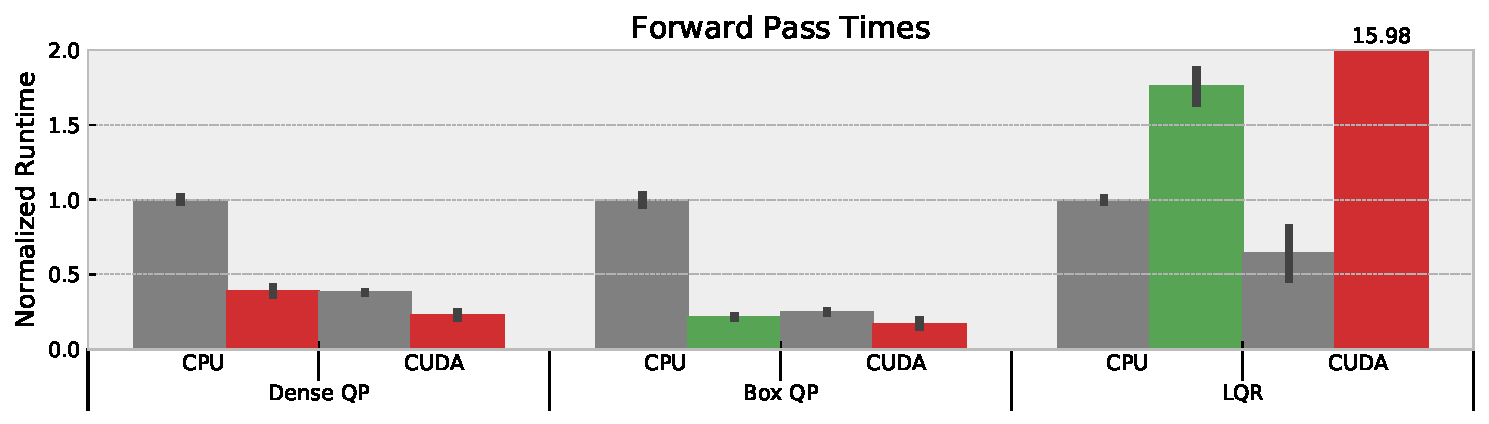
\includegraphics[width=0.9\textwidth]{prof/forward-summary.pdf} \\
  \cblock{128}{128}{128} Specialized Solver \enskip
  \cblock{208}{46}{47} PyTorch Block Direct \enskip
  \cblock{86}{165}{84} SCS Serial Direct
  \caption{
    Forward pass execution times.
    For each task we run ten trials
    on an unloaded system and normalize the runtimes to the
    CPU execution time of the specialized solver.
    The bars show the 95\% confidence interval.
    For our method, we show the best performing mode.
  }
  \label{fig:eval:fwd}
\end{figure}

\begin{figure}[!h]
  \centering
  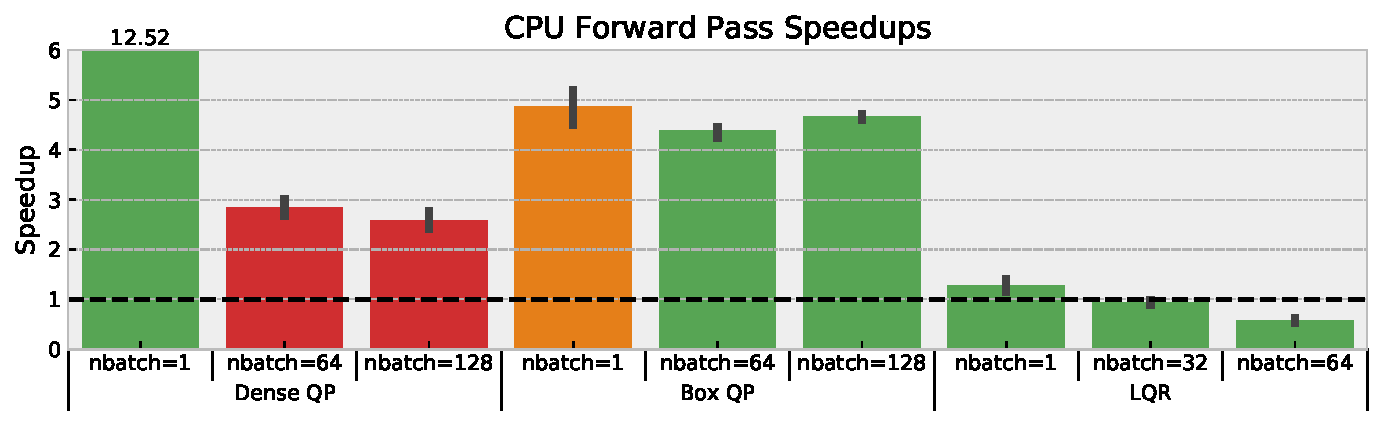
\includegraphics[width=0.9\textwidth]{prof/CPU-forward-speedups.pdf}
  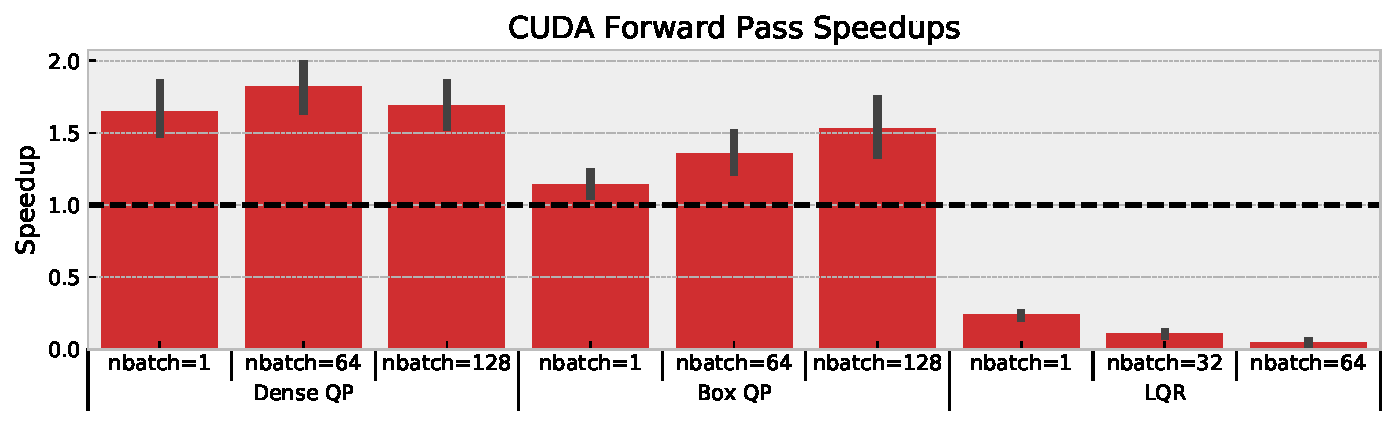
\includegraphics[width=0.9\textwidth]{prof/CUDA-forward-speedups.pdf}

  \cblock{208}{46}{47} PyTorch Block Direct \enskip
  \cblock{86}{165}{84} SCS Serial Direct \enskip
  \cblock{230}{127}{25} SCS Block Direct

  \caption{
    Forward pass execution time speedups of our best
    performing method in comparison to the specialized
    solver's execution time.
    For each task we run ten trials on an unloaded system.
    The bars show the 95\% confidence interval.
  }
  \label{fig:eval:fwd:speedups}
\end{figure}

\begin{figure}[!h]
  \centering
  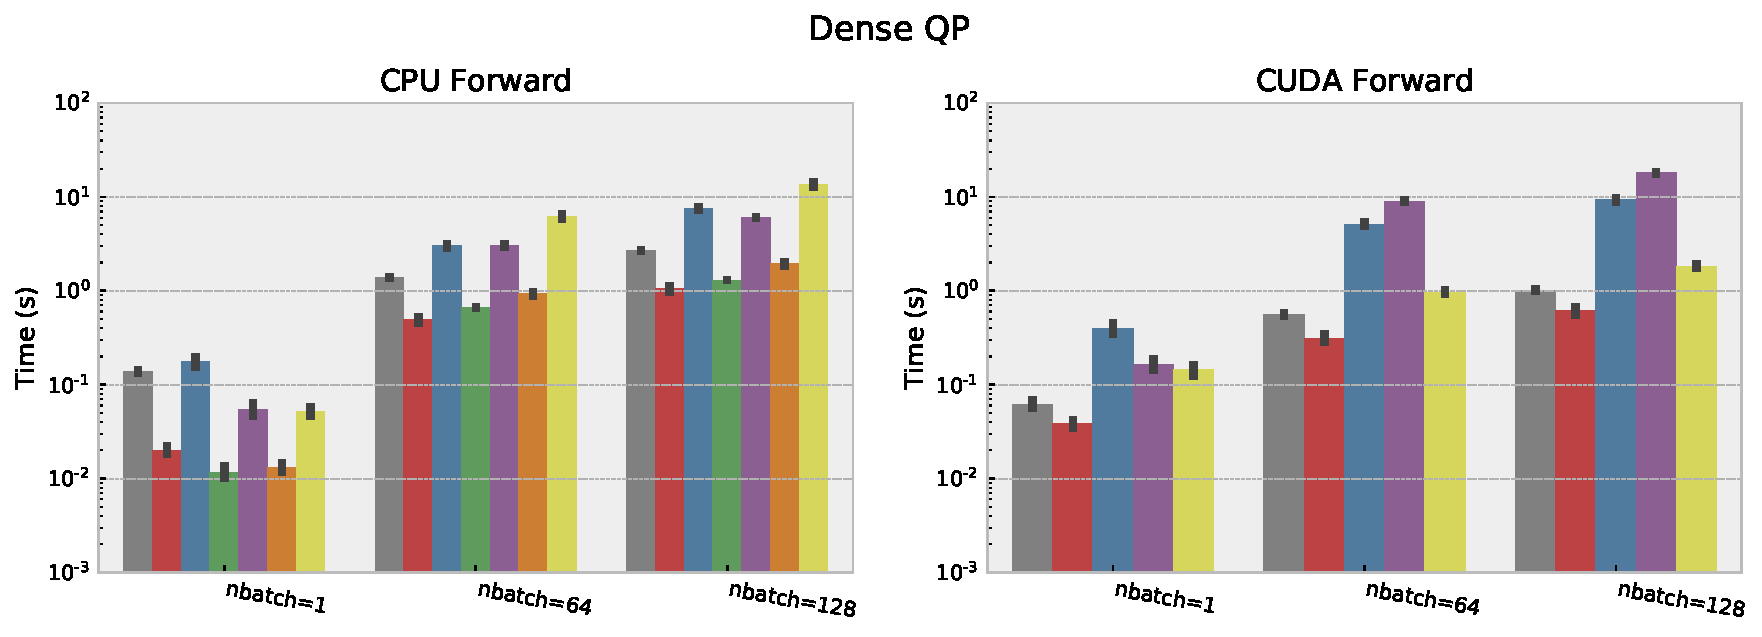
\includegraphics[width=0.9\textwidth]{prof/prof_qp_dense-forward.pdf}
  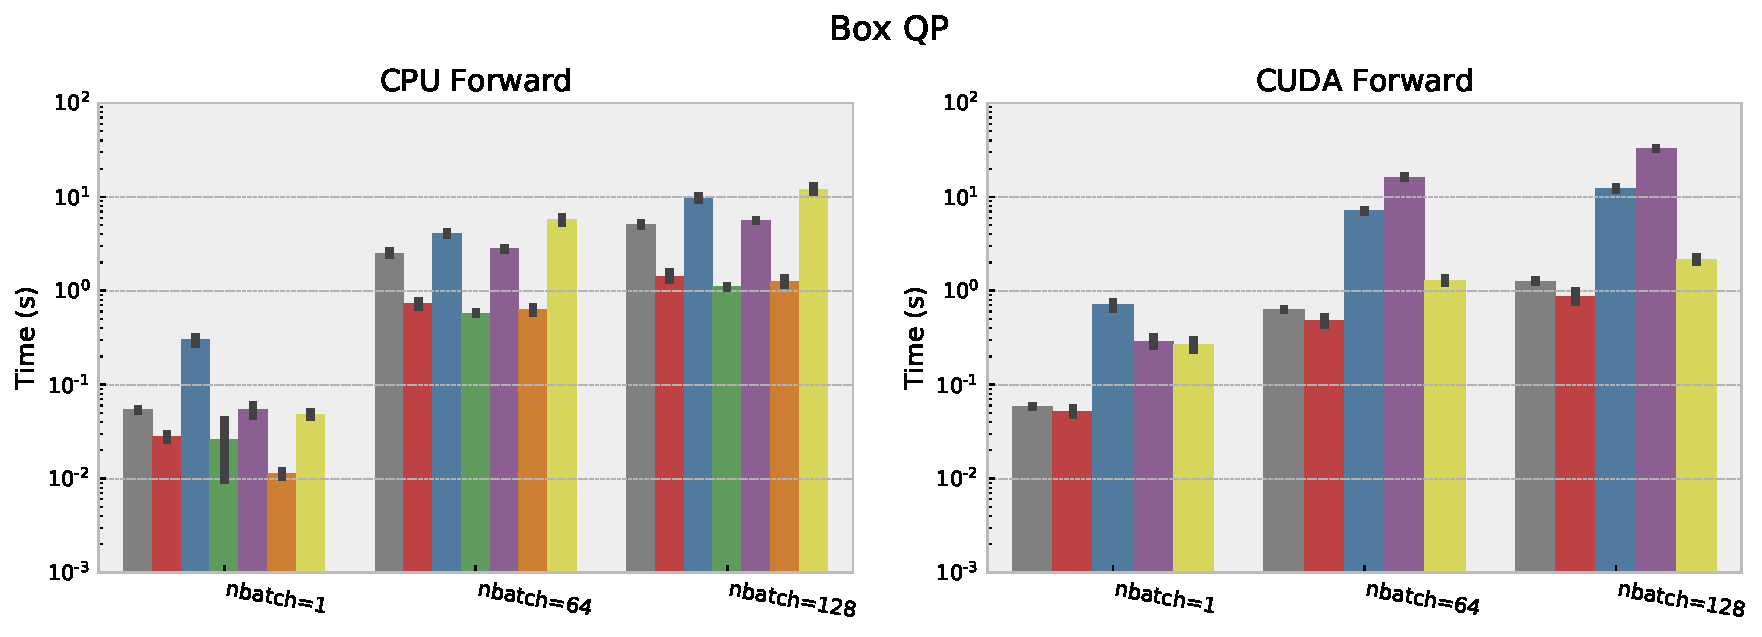
\includegraphics[width=0.9\textwidth]{prof/prof_qp_box-forward.pdf}
  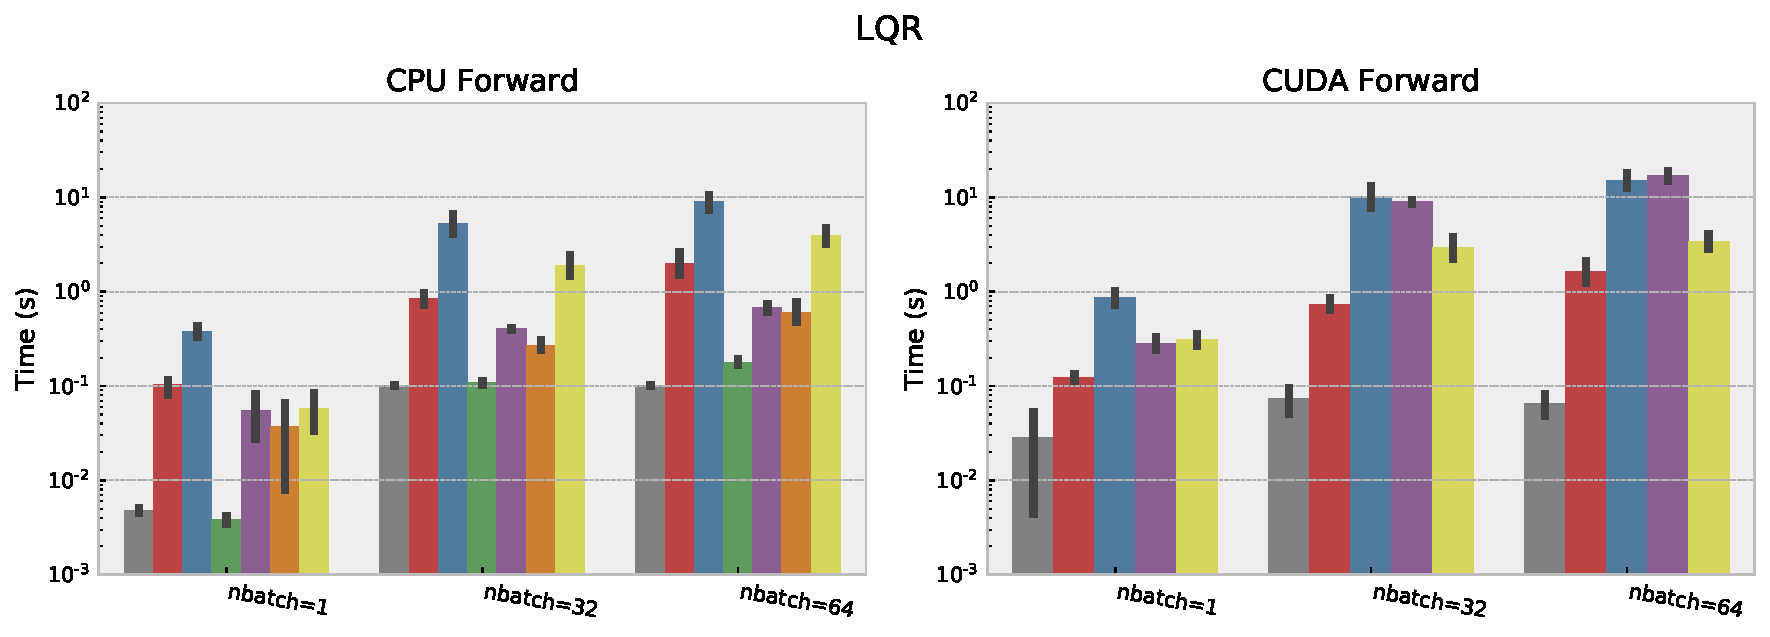
\includegraphics[width=0.9\textwidth]{prof/prof_mpc-forward.pdf}

  \cblock{128}{128}{128} Specialized Solver \enskip
  \cblock{208}{46}{47} PyTorch Block Direct \enskip
  \cblock{68}{125}{171} PyTorch Block Indirect \\
  \cblock{86}{165}{84} SCS Serial Direct \enskip
  \cblock{146}{86}{155} SCS Serial Indirect \enskip
  \cblock{230}{127}{25} SCS Block Direct \enskip
  \cblock{235}{235}{71} SCS Block Indirect

  \caption{Full data for the forward pass execution times.
    For each task we run ten trials on an unloaded system.
    The bars show the 95\% confidence interval.
  }
  \label{fig:eval:fwd:all}
\end{figure}

\newpage~\newpage~\newpage
\subsection{Backward pass profiling}
\label{sec:cvxpyth:bw_prof}
In this section we compare the backward pass times of
our layer in comparison to the specialized solvers
on the same three tasks as before: the dense QP,
the box QP, and LQR.
We show that differentiating through our conic
solver is competitive in comparison to the
specialized solver.
As a comparison point, the \qpth solver exploits
the property that the linear system for the backward pass is the
same as the linear system in the forward pass and can therefore
do the backward pass with a single pre-factorized solve.
The LQR solver exploits the property that the backward
pass for LQR can be interpreted as another LQR problem that
can efficiently be solved with the Riccati recursion.

These comparisons are important because the linear system for
differentiating cone programs in \cref{eq:cvxpyth:diff_efficient}
is a more general form and cannot leverage the same exploits
as the specialized solvers.
To get an intuition of what these linear systems look like on
our tasks, we plot sample maps on smaller problems of the
coefficient matrix in \cref{fig:cvxpyth:sample_maps}.
This illustrates the sparsity that is typically present in the
linear system that needs to be solved, but also illustrates
that beyond sparsity, there is no other common property that
can be exploited between the tasks.

\begin{figure}[!t]
  \centering
  \includegraphics[height=2.0in]{Ms_qpth_dense.pdf}
  \includegraphics[height=2.0in]{Ms_qpth_box.pdf}
  \includegraphics[height=2.0in]{Ms_MPC.pdf}
  \caption{Sample linear system coefficients for
    the backward pass system in \cref{eq:cvxpyth:diff_efficient}
    on smaller versions of the tasks we consider.
    The tasks we consider are approximately five
    times larger than these systems.
  }
  \label{fig:cvxpyth:sample_maps}
\end{figure}

To understand how many LSQR iterations are necessary
to solve our task, we compare the approximate derivatives computed
by LSQR to the derivatives obtained by directly solving
the linear system in \cref{fig:cvxpyth:lsqr_conv}.
This shows that typically 500-1000 LSQR iterations
are necessary for the tasks that we consider.
In some cases such as $\partial x^\star / \partial A$
for LQR, the approximate gradient computed by LSQR does
never converges exactly to the true gradient.

\begin{figure}[!t]
  \centering
  \includegraphics[width=0.9\textwidth]{lsqr_dense_qp.pdf}
  \includegraphics[width=0.9\textwidth]{lsqr_box_qp.pdf}
  \includegraphics[width=0.9\textwidth]{lsqr_mpc.pdf}

  \cblock{68}{125}{171} $\partial x^\star/\partial A$ \enskip
  \cblock{208}{46}{47} $\partial x^\star / \partial b$ \enskip
  \cblock{146}{86}{155} $\partial x^\star / \partial c$
  \caption{LSQR convergence for the backward pass systems.
    The shaded areas show the 95\% confidence interval
    across ten problem instances.
  }
  \label{fig:cvxpyth:lsqr_conv}
\end{figure}

\begin{figure}[!t]
  \centering
  \includegraphics[width=0.9\textwidth]{prof/prof_qp_dense-backward.pdf}
  \includegraphics[width=0.9\textwidth]{prof/prof_qp_box-backward.pdf}
  \includegraphics[width=0.9\textwidth]{prof/prof_mpc-backward.pdf}

  \cblock{128}{128}{128} Specialized Solver \enskip
  \cblock{208}{46}{47} Direct (Dense) \enskip
  LSQR
  (\cblock{68}{125}{171} 100 \cblock{86}{165}{84} 500 \cblock{146}{86}{155} 1000)
  Iterations
  \caption{
    Backward pass execution times.
    For each task we run ten trials on an unloaded system.
    The bars show the 95\% confidence interval.
  }
  \label{fig:cvxpyth:bw}
\end{figure}

\newpage~\newpage~\newpage
\cref{fig:cvxpyth:bw} compares our backward pass times to
the specialized solvers for the QP and LQR tasks.
This shows that there is a slight computational overhead
in comparison to the specialized solvers, but that
solving the linear system is still tractable for these tasks.
The LSQR runtime is serialized across the batch, and is
currently only implemented on the CPU.
We emphasize that if the backward pass time becomes a bottleneck,
the runtime can be further improved by further exploiting the
sparsity by investigating other direct and indirect solvers
for the systems, or by exploiting the property that we mentioned
earlier in \cref{sec:diff-cp} that for simple cones like the
free and non-negative cones, parts of the system become the same as
parts of the KKT system.

\section{Conclusion}
This section has presented a way of differentiating through
cone programs that enabled us to create a powerful prototyping
tool for differentiable convex optimization layers.
Practitioners can use this library in place of hand-implementing
a solver and implicitly differentiating the KKT conditions.
The speed of our tool is competitive with the speed of specialized
solvers, even in the batched setting required for machine learning.

%%% Local Variables:
%%% coding: utf-8
%%% mode: latex
%%% TeX-engine: xetex
%%% TeX-master: "../thesis"
%%% End:

\part{Conclusions and Future Directions}
\chapter{Conclusions and Future Directions}
\label{sec:conclusions}

In this thesis we have introduced new building blocks and
fundamental components for machine learning that enable
optimization-based domain knowledge to be injected
into the modeling pipeline.
We have presented the \emph{OptNet} architecture as a
foundation for convex optimization layers and the
\emph{input-convex neural network} architecture as a
foundation for deep convex energy-based learning.
We have shown how the OptNet approach can be applied to
differentiable model-predictive control and
top-$k$ learning.
To enable rapid prototyping in this space, we have shown
how \cvxpy can be turned into a differentiable layer.
Differentiable optimization provides an expressive set of
operations and have a promising set of future directions.
In the following we provide a brief outlook of how optimization-based
modeling benefits seven application areas,
and we highlight a few key references in this space.

\begin{enumerate}
\item \textbf{Game theory.}
  The game theory literature typically focuses on finding
  optimal strategies of playing games with known rules.
  While the rules of a lot of games are known explicitly,
  scenarios could come up where it's useful to learn the
  rules of a game and to have a ``game theory''
  equilibrium-finding layer.
  For example in reinforcement learning, an agent can have an
  arbitrary differentiable ``game theory'' layer that is able
  of representing complex tasks, state spaces, and
  problems as an equilibrium-finding problem in a game
  where the rules are automatically extracted.
  This is explored in
  \citet{ling2018game}.
\item \textbf{Stochastic optimization and end-to-end learning.}
  Typically probabilistic models are used in the context of
  larger systems. When these systems have an objective
  that is being optimized, it is usually ideal to incorporate
  the knowledge of this objective into the probabilistic modeling
  component.
  If the downstream systems involve solving
  stochastic optimization problems, as in power-systems,
  creating an end-to-end differentiable architecture is
  more difficult and can be done by using
  differentiable optimization as in \citet{donti2017task}.
  \newpage
\item \textbf{Reinforcement learning and control.}
  \begin{itemize}
  \item \textbf{Safety.} RL agents may be deployed in scenarios when
    the agent should avoid parts of the state space,
    \eg in safety-critical environments.
    Differentiable optimization layers can be used
    to help constrain the policy class so that these
    regions are avoided.
    This is explored in
    \citet{dalal2018safe,pham2018optlayer}.
  \item \textbf{Differentiable control and planning.}
    The differentiable MPC approach we presented in \cref{sec:empc}
    is just one step towards a significantly broader vision
    of integrating control and learning for doing imitation
    or policy learning.
  \item \textbf{Physics-based modeling.}
    When RL environments involve physical systems,
    it may be useful to have a physics-based modeling.
    This can be done with a differentiable
    physics engines as in \citet{de2018end}.
  \item \textbf{Inverse cost and reward learning.}
    Given observed trajectories in an imitation learning
    setup, modeling agents as controllers that are
    optimizing an objective is a powerful paradigm
    \citep{ng2000algorithms,finn2016guided}.
    Differentiable controllers
    are useful when trying to reconstruct an optimization
    problem that other agents are solving.
    This is done in the context of cost shaping in
    \citet{tamar2017learning}.
  \item \textbf{Multi-agent environments.}
    In multi-agent environments, other agents can be modeled
    as entities that are solving control optimization or
    other learning problems.
    This knowledge can be integrated into the learning
    procedure as in \citet{foerster2018learning}.
  \item \textbf{Control in high-dimensional state spaces.}
    Control in high-dimensional state spaces such as visual
    spaces is challenging and it is typically useful
    to extract a lower-dimensional latent space from
    the original feature space.
    This is typically done by either hand-engineering
    a feature extractor, or by learning an embedding
    with an unsupervised learning method as in
    \citet{watter2015embed,kurutach2018learning}.
    Viewing controllers as differentiable entities is
    reasonable for embedding states because the cost
    function of the controller can be parameterized to
    learn a cost associated with the latent representation.
  \end{itemize}
\item \textbf{Discrete, combinatorial, and submodular optimization.}
  The space of discrete, combinatorial, and mixed optimization problems
  captures an even more expressive set of operations than
  the continuous and convex optimization problems we have considered
  in this thesis.
  Similar optimization components can be made for some of these
  types of problems and is explored in
  \citet{djolonga2017differentiable,tschiatschek2018differentiable,mensch2018differentiable,niculae2018sparsemap,niculae2017regularized}.
  \newpage
\item \textbf{Meta-learning.}
  Some meta-learning formulations such as \citet{finn2017model}
  and \citet{ravi2016optimization}
  involve learning through an unrolled optimizer that
  typically solve an unconstrained, continuous, and
  non-convex optimization problem.
  In some cases, unrolling through a solver with
  many iterations may require inefficient amounts
  of compute or memory.
  Meta-learning methods can be improved by using
  differentiable closed-form solvers, as done in
  MetaOptNet \citep{lee2019meta} with a differentiable SVM layer
  and in \citet{bertinetto2018meta} with differentiable ridge
  and logistic regression.
\item \textbf{Optimization viewpoints of standard components.}
  A motivation behind this thesis work has been the optimization
  viewpoints of standard layers we discussed in \cref{sec:bg:existing}.
  Many other directions can be taken with the viewpoints, such
  as the proximal operator viewpoint in \citet{bibi2018deep}
  that interprets deep layers as stochastic solvers.
\item \textbf{Hyper-parameter and generalization optimization.}
  The learning procedure for many linear machine learning models
  can be interpreted as the solution to a convex
  optimization problem over the loss function.
  This convex learning process can therefore also be
  made differentiable and used for optimizing the hyper-parameters
  of these algorithms. This is done in
  \citet{barratt2018optimizing} to optimize the cross-validation
  risk of convex formulations, including logistic regression,
  SVMs, and elastic net regression;
  for least squares in \citet{barratt2019least};
  and SVMs in \citet{lee2019meta}.
\end{enumerate}

%%% Local Variables:
%%% coding: utf-8
%%% mode: latex
%%% TeX-engine: xetex
%%% TeX-master: "../thesis"
%%% End:

\chapter*{Bibliography}
\addcontentsline{toc}{chapter}{Bibliography}

\vspace{-25mm}
This bibliography contains \total{citenum} references.
\vspace{10mm}

\printbibliography[heading=none]

\end{document}

%%% Local Variables:
%%% coding: utf-8
%%% mode: latex
%%% TeX-engine: xetex
%%% End:
